\documentclass{beamer} %[handout]
\usepackage[utf8]{inputenc}
\usepackage[T1]{fontenc}
\usepackage[italian]{babel}
\usepackage{siunitx}
\usepackage{amsmath, amssymb, mathtools,bm} 					%matematica
\usepackage{import} 							%inkscape
\usepackage{booktabs}
\usepackage{multirow}
\usepackage{threeparttable}	
\usepackage[english,nowave]{PadovaThesis}
%\input{PadovaThesis.sty}

\newcommand{\sun}{\ensuremath{_\odot}} 	

\renewcommand{\assistantsize}{\normalsize}

\titolo{\normalfont  Wolf-Rayet -- black hole binaries as progenitors of binary black holes}
\titoletto{\vspace*{-8mm}\scriptsize Master Degree in Astrophysics and Cosmology}
\candidato{Erika Korb}
\relatore{Prof. Michela Mapelli}
\correlatore{Dr.~Giuliano Iorio}
\data{$21^{\rm st}$ September 2022}


\begin{document}
\begin{frame}
	\maketitle
\end{frame}




\begin{frame}{Explaining gravitational wave detections}
	\centering
	\evidenzia{\textbf{Which are the evolutionary channels of the $\sim$ 90 compact object binaries observed with gravitational wave detectors?}}
	\bigskip

	\centering
	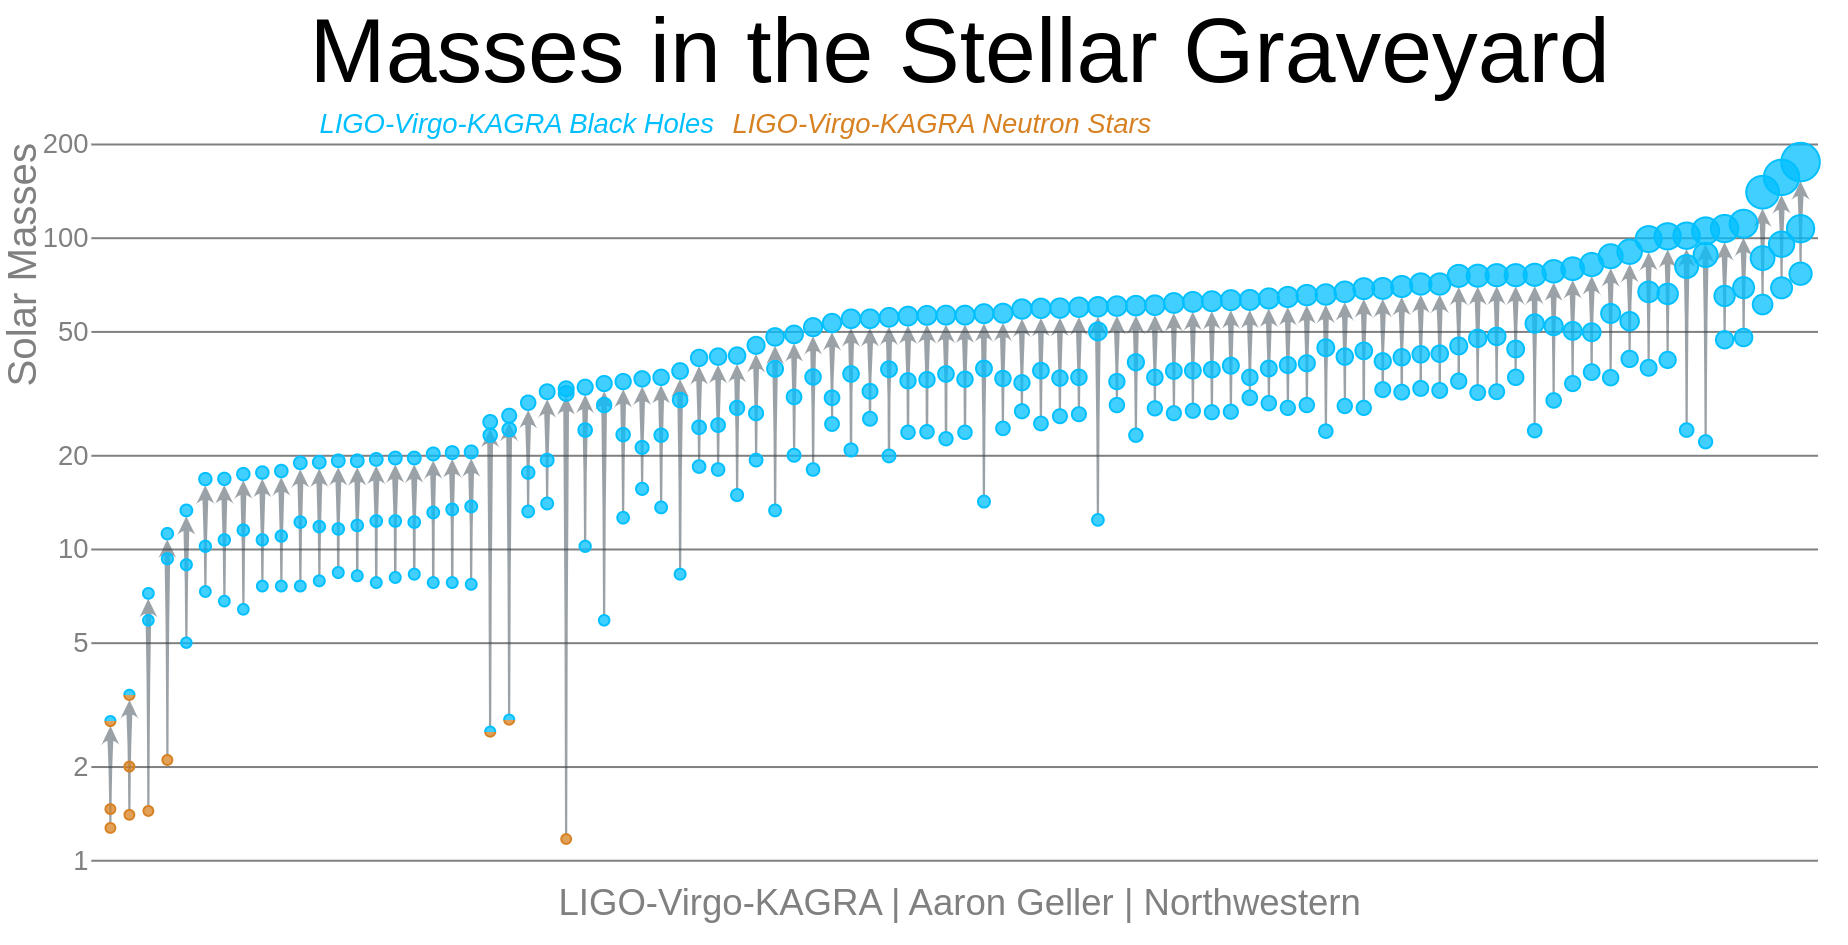
\includegraphics[width=.95\textwidth]{./images/GWTC3MassWhite.png}
	\flushright
	\referenza{The LIGO-Virgo-KAGRA Collaboration 2021}

\end{frame}


\begin{frame}{Limited state-of-the-art models}
	\scriptsize
	\begin{columns}
		\begin{column}{0.4\textwidth}	
			\evidenzia{\textbf{Probable evolution}}:
			\smallskip
			\begin{enumerate}
				\item Isolated binary
				\item \textbf{Mass transfer (?)}
				\item \textbf{Supernova}
				\item Black hole + star
				\item \textbf{Mass transfer}
				\item \textbf{Supernova}
				\item Binary black hole (BBH)
				\item Merging via GW emission
			\end{enumerate}
		\vspace{.4cm}	
		\end{column}
		\begin{column}{0.7\textwidth}
			\centering
				\def\svgwidth{\textwidth}
			\import{./images/}{cartoon_binary.pdf_tex}
		\end{column}
	\end{columns}
	\bigskip
	\smallskip
	\begin{columns}
		\begin{column}{0.45\textwidth}
		\evidenzia{\textbf{Uncertainties:}}
		\begin{itemize}
			\item \textbf{Mass transfer}
			\item \textbf{Core-collapse supernova} 
			\item \textbf{Supernova kick}
		\end{itemize}	
		\end{column}
		\begin{column}{0.65\textwidth}
			\flushleft
			\textbf{$\sim$ 80 merging BBHs detected...}
			\medskip
			\flushright
			\textbf{...can we observe their progenitors?}
		\end{column}
	\end{columns}
	
\end{frame}




\begin{frame}{Wolf-Rayet -- black hole binaries}
	\scriptsize
	\begin{columns}
		\begin{column}{0.72\textwidth}
			\evidenzia{\textbf{Wolf-Rayet stars: }}
			\begin{itemize}
				\item Strong stellar winds ($\dot{M} \sim 10^4-10^5~M_\odot~\text{yr}^{-1}$)
				\item \textbf{Little or no H envelope} $\rightarrow$ \textbf{mass transfer product?}
				\item $R_{\text{WR}} \sim R_\odot$ $\rightarrow$ \textbf{allow close orbits} $a \gtrsim R_\odot$ $\rightarrow$ \textbf{merging?}
			\end{itemize}
		\end{column}
		\begin{column}{0.34\textwidth}
			\centering
			\evidenzia{\textbf{Time to merge only via GW emission}}
			\[t_{\text{GW}}~^* \sim 12~\text{Gyr}~\left(\frac{a}{20~ R_\odot}\right)^4\]
			\referenza{Peters 1964}
		\end{column}
	\end{columns}
	\bigskip

	\centering
	\evidenzia{\small \textbf{Only 7 known Wolf-Rayet -- black hole candidates}}
	\bigskip
	
	\begin{threeparttable}
	\begin{tabular}{llcccc}
		\toprule
		\multirow{2}{*}{Host galaxy} & \multirow{2}{*}{Name} & $M_{\text{BH}}$ & $M_{\text{WR}}$ & $P$ & $t_{\text{GW}}~^*$ \\
		& & [$M_\odot$] & [$M_\odot$] & [hours] & [Gyr] \\
		\midrule
		\textbf{Milky Way} & \textbf{Cyg X-3} & \textbf{3-10} & \textbf{8-14} & \textbf{4.8} & \textbf{0.02} \\
		IC 10 & IC10 X-1 & - & 17-35 & 34.9 & 3.5 \\
		NGC 300 & NGC300 X-1 & 13-21 & 15-26 & 32.8 & 2.9 \\
		NGC 253 & CXOU J004732.0-251722.1 & - & - & 14.5 & 0.3  \\
		Circinus & CG X-1 & - & - & 7.2  & 0.05 \\
		M101 & M101 ULX-1 & 8-46 & 17-19 & 196.8 & 348 \\
		NGC 4490 & CXOU J123030.3+413853 & - & - & 6.4 & 0.04 \\
		\bottomrule 	
	\end{tabular}
	\begin{tablenotes}[para]
	\tiny
	$^*~t_{\text{GW}}$ estimated with Peters 1964, assuming circular orbit and $M_1 = M_2 = 10~M_\odot$
	\end{tablenotes}
	\end{threeparttable}
	\flushright
	\vspace{-2mm}
	\referenza{Esposito et al. 2015, Koljonen et al. 2017}
\end{frame}

\begin{frame}{Goals and methodology of the thesis}
	\small
	
	\evidenzia{\textbf{Goals:}}\\
	\begin{enumerate}		
		\item \textbf{Wolf-Rayet -- black hole:} progenitors of merging BBHs at $Z_\odot$?
		\item \textbf{Cyg X-3:} case-study for evolution of merging BBHs at $Z_\odot$
	\end{enumerate}

	\bigskip
	\bigskip
	\centering
	\evidenzia{\textbf{Model-independent results? $\rightarrow$ 24 combinations of parameters}}
	\flushleft
	\bigskip
	\medskip

	\evidenzia{\textbf{Methodology:}}
	\begin{itemize}
		\item I generated \textbf{24 sets of} $\textbf{10}^{\textbf{6}}$ \textbf{binaries} $\rightarrow$ initial conditions \textbf{representative} of early-binaries observed in the Milky Way\\
		\referenza{Sana et al. 2012, Moe \& Di Stefano 2017}
		\medskip
		\item \textbf{Simulations with the population-synthesis code \texttt{SEVN}} \\
		(\emph{Stellar EVolution for N-body simulations})\\
		\referenza{Spera et al. 2019, Costa et al. 2021, Iorio et al. in prep.}
	\end{itemize}
\end{frame}



\begin{frame}{Parameter space in \texttt{SEVN}}
		\begin{columns}
		\begin{column}{0.9\textwidth}
			\flushright
			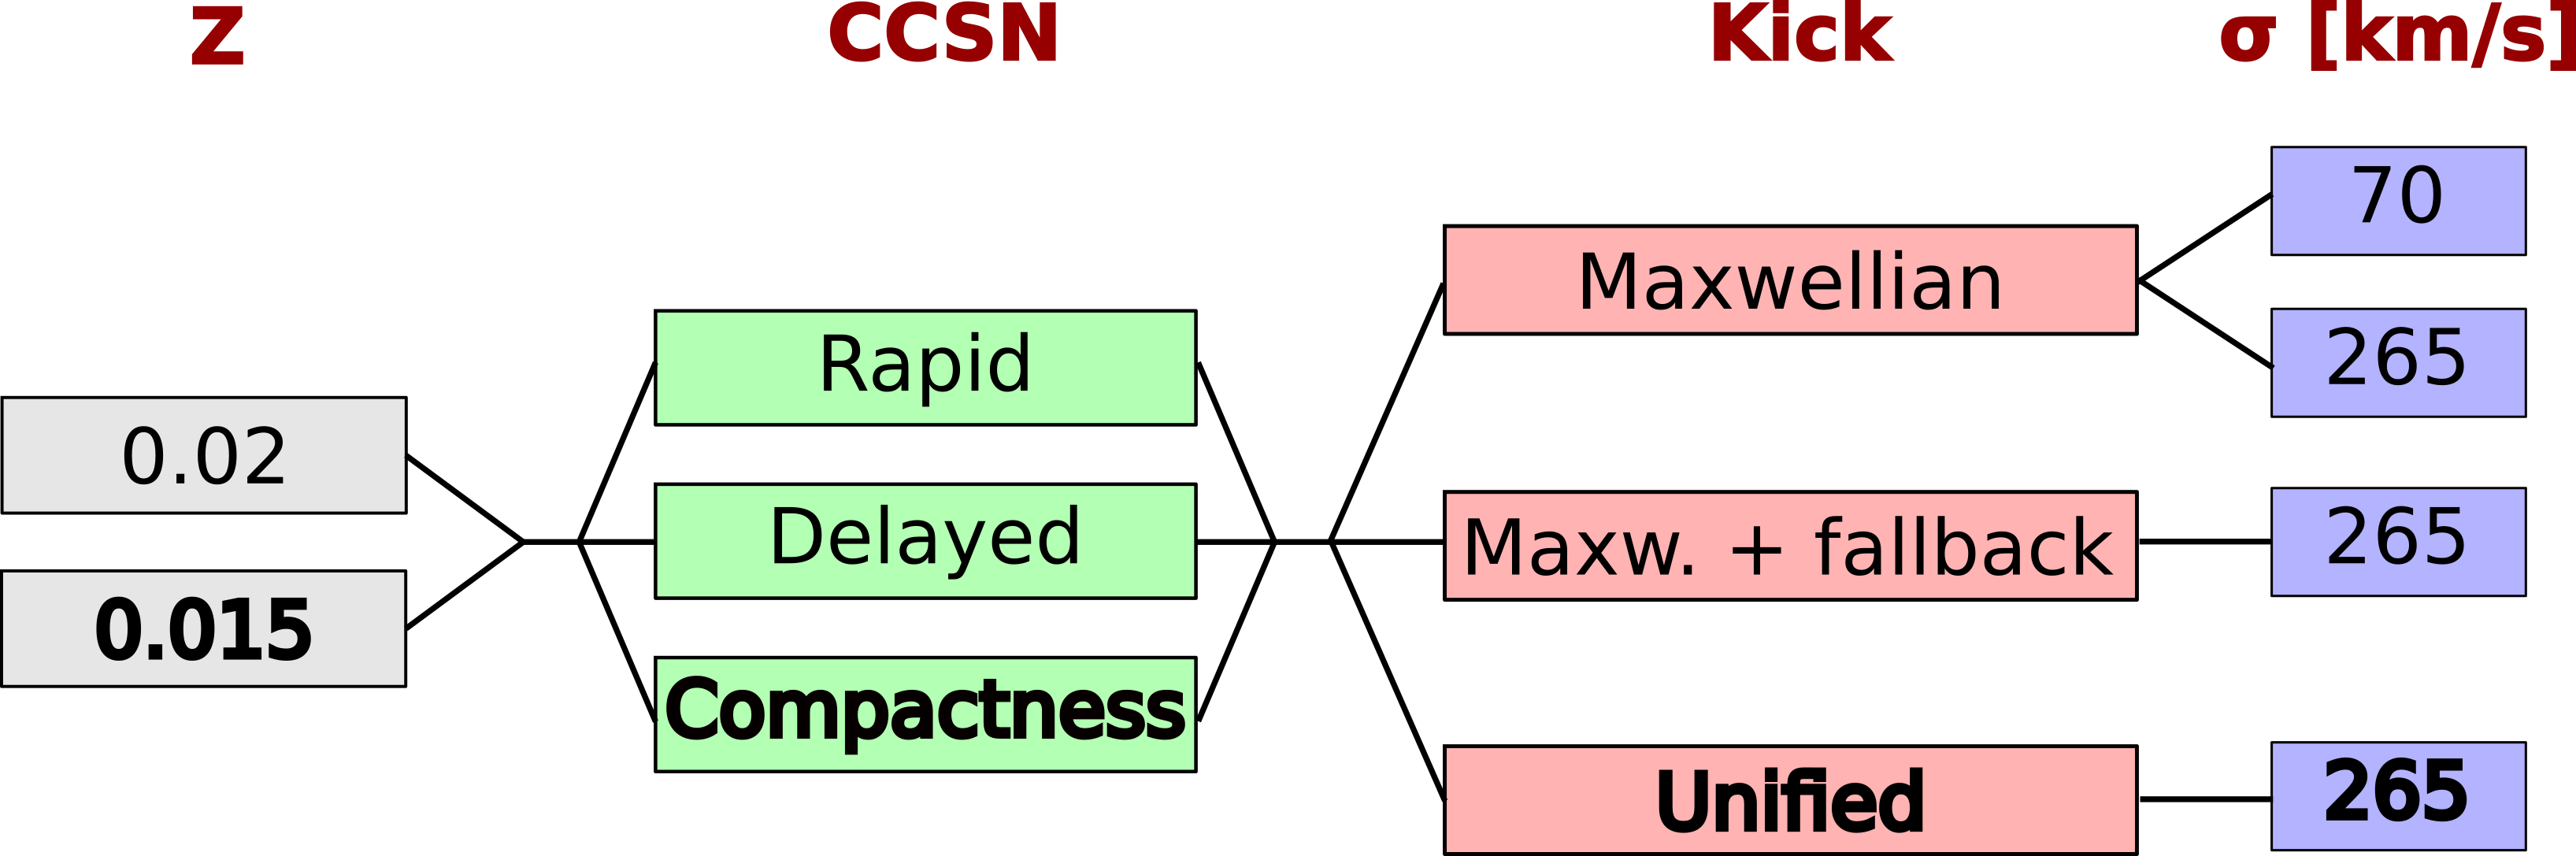
\includegraphics[width=\textwidth]{./images/parameterspace.png}
		\end{column}
		\begin{column}{0.25\textwidth}
			\scriptsize
			$\rightarrow$: BBHs\\
			\referenza{Atri et al. 2019}\\
			$\rightarrow$: Young pulsars \\
			\referenza{Hobbs et al. 2005}\\
			\smallskip
			$\rightarrow$ Fallback re-scaling\\ \referenza{Fryer et al. 2012}\\
			\smallskip
			$\rightarrow$ Linear momentum \\ \referenza{Giacobbo \& Mapelli 2020}\\
			\vspace{-10mm}
		\end{column}	
	\end{columns}
	\medskip
	\begin{columns}
		\begin{column}{0.47\textwidth}			
			\scriptsize
			\evidenzia{\textbf{Core-collapse supernova (CCSN)}}\\
			\bigskip
			Preference for compact object masses:\\
			\medskip
			\begin{itemize}
				\item Light (Rapid/Delayed)\\ \referenza{Fryer et al. 2012}
				\smallskip
				\item Heavy (Compactness)\\ \referenza{Mapelli et al. 2020}
			\end{itemize}
		\end{column}
		\begin{column}{0.6\textwidth}
			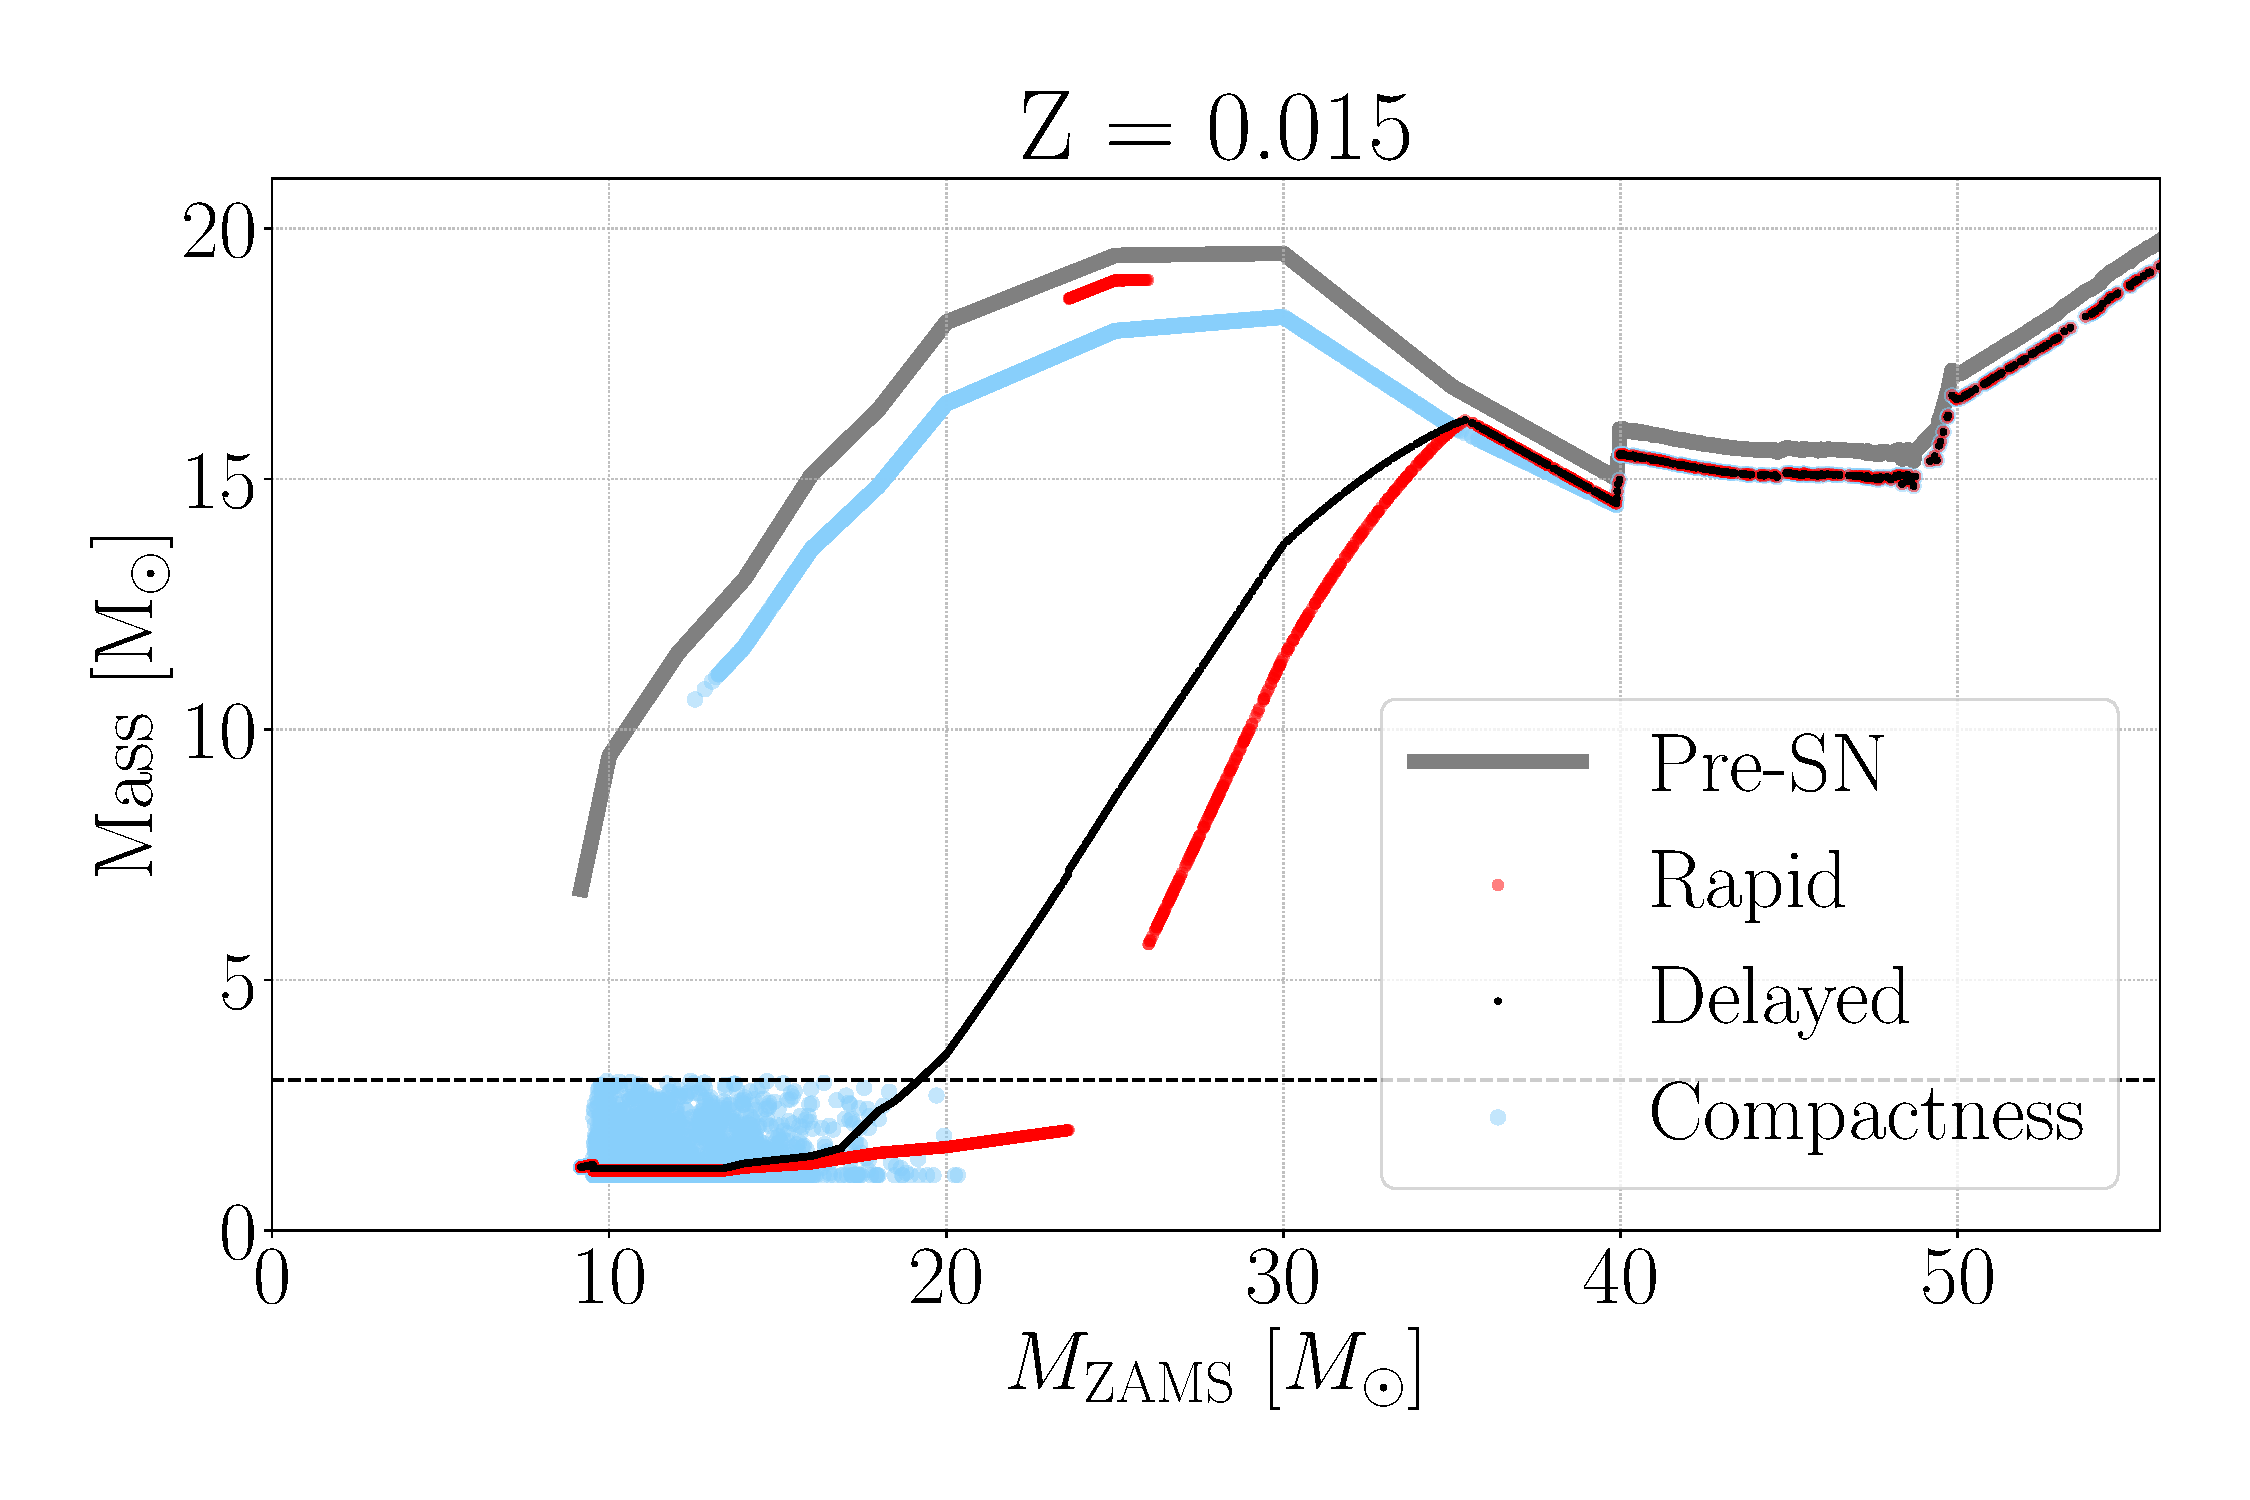
\includegraphics[width=\textwidth]{./images/remnants_Z015_cut.pdf}
		\end{column}	
	\end{columns}
	
\end{frame}



\begin{frame}{Results: key progenitors at $\boldsymbol{Z_\odot}$}
	
	\small
	\begin{columns}
		\begin{column}{1.05\textwidth}
			\evidenzia{\textbf{Main results:}}
			\smallskip
			\begin{enumerate}
				\item Wolf-Rayet -- black hole: required for merging BBHs at $\boldsymbol{Z_\odot}$\\
				($\bm{\gtrsim} \textbf{90}\%$ \textbf{probability}) 
				\item Cyg X-3:  progenitor of merging BBHs \\ ($\bm{\gtrsim} \textbf{75}\%$ \textbf{probability}) 
			\end{enumerate}
		\end{column}	
	\end{columns}

	\begin{columns}
	\begin{column}{0.4\textwidth}
		\evidenzia{\textbf{In this parameter space:}}\\
		\begin{itemize}
			\item Results almost model-independent		
			\item Cyg X-3 represents a sub-population of merging BBHs progenitors
			%\vspace{5mm}
		\end{itemize}
	\end{column}
	\begin{column}{0.6\textwidth}
		%\hspace{-2cm}
		\vspace{3mm}
		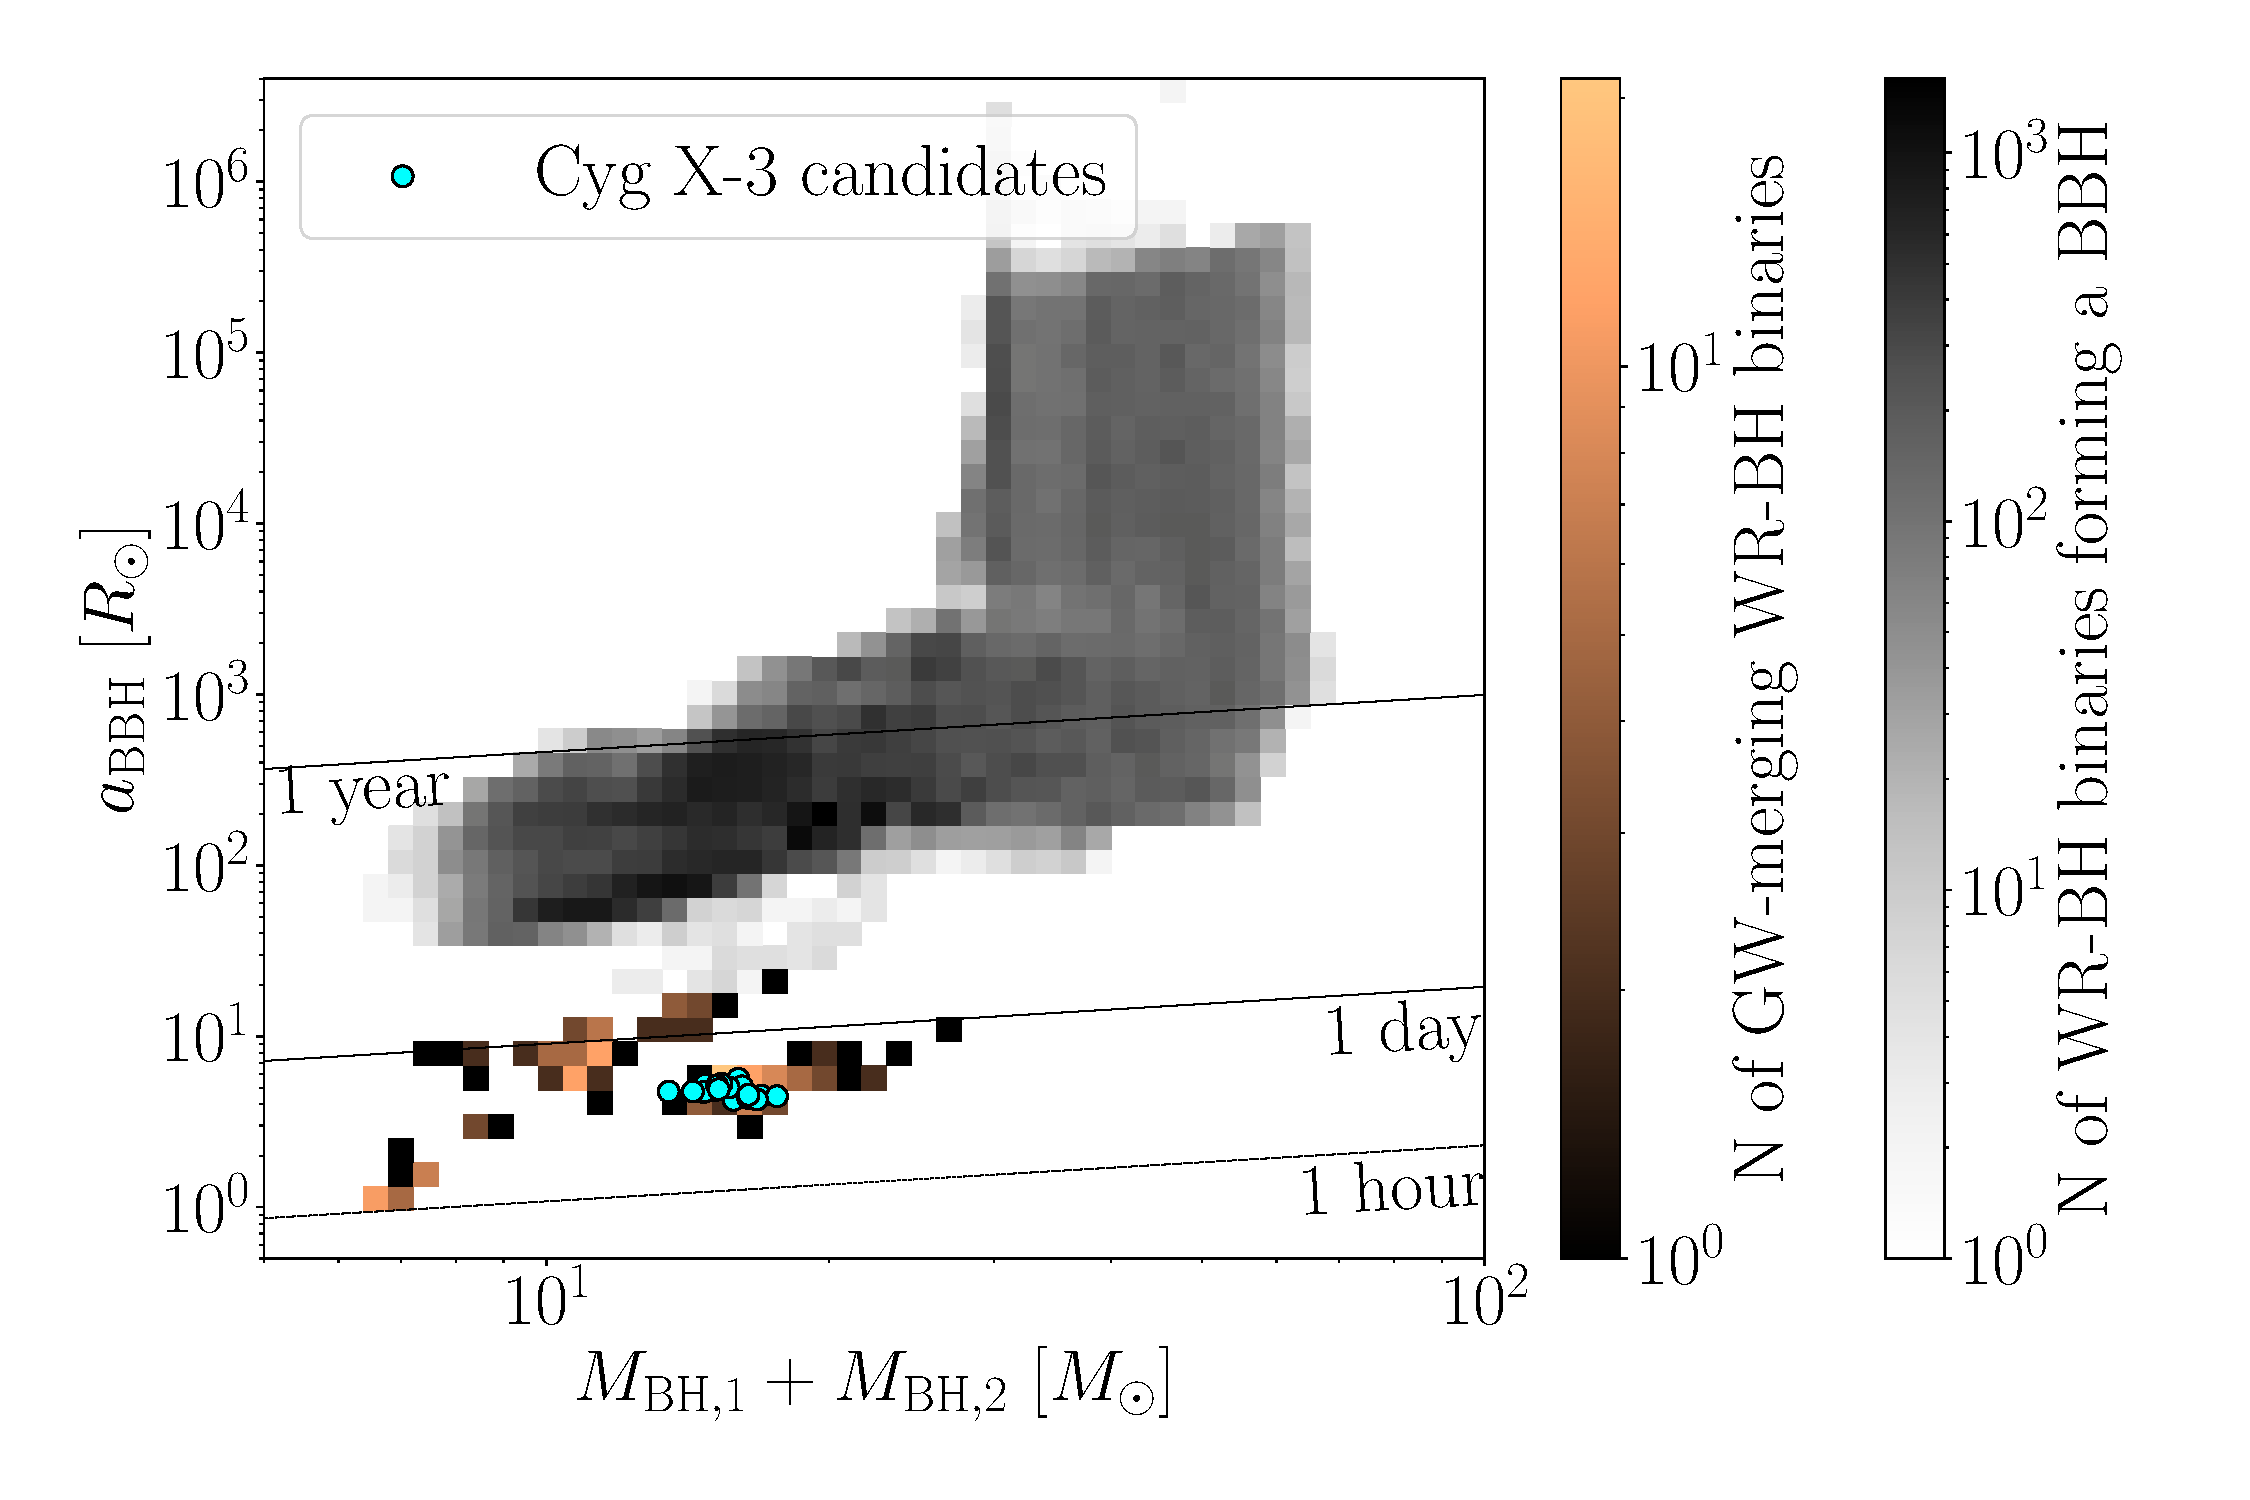
\includegraphics[width=\textwidth]{./images/avsMtotREMBHBH_GW_WRBH_BHBH_GW_WRBH_cyg_x-3--Ko17.pdf}
	\end{column}	
\end{columns}
\end{frame}

\begin{frame}{Probing the parameter space at Z=0.015}
		\begin{columns}
		\begin{column}{0.9\textwidth}
			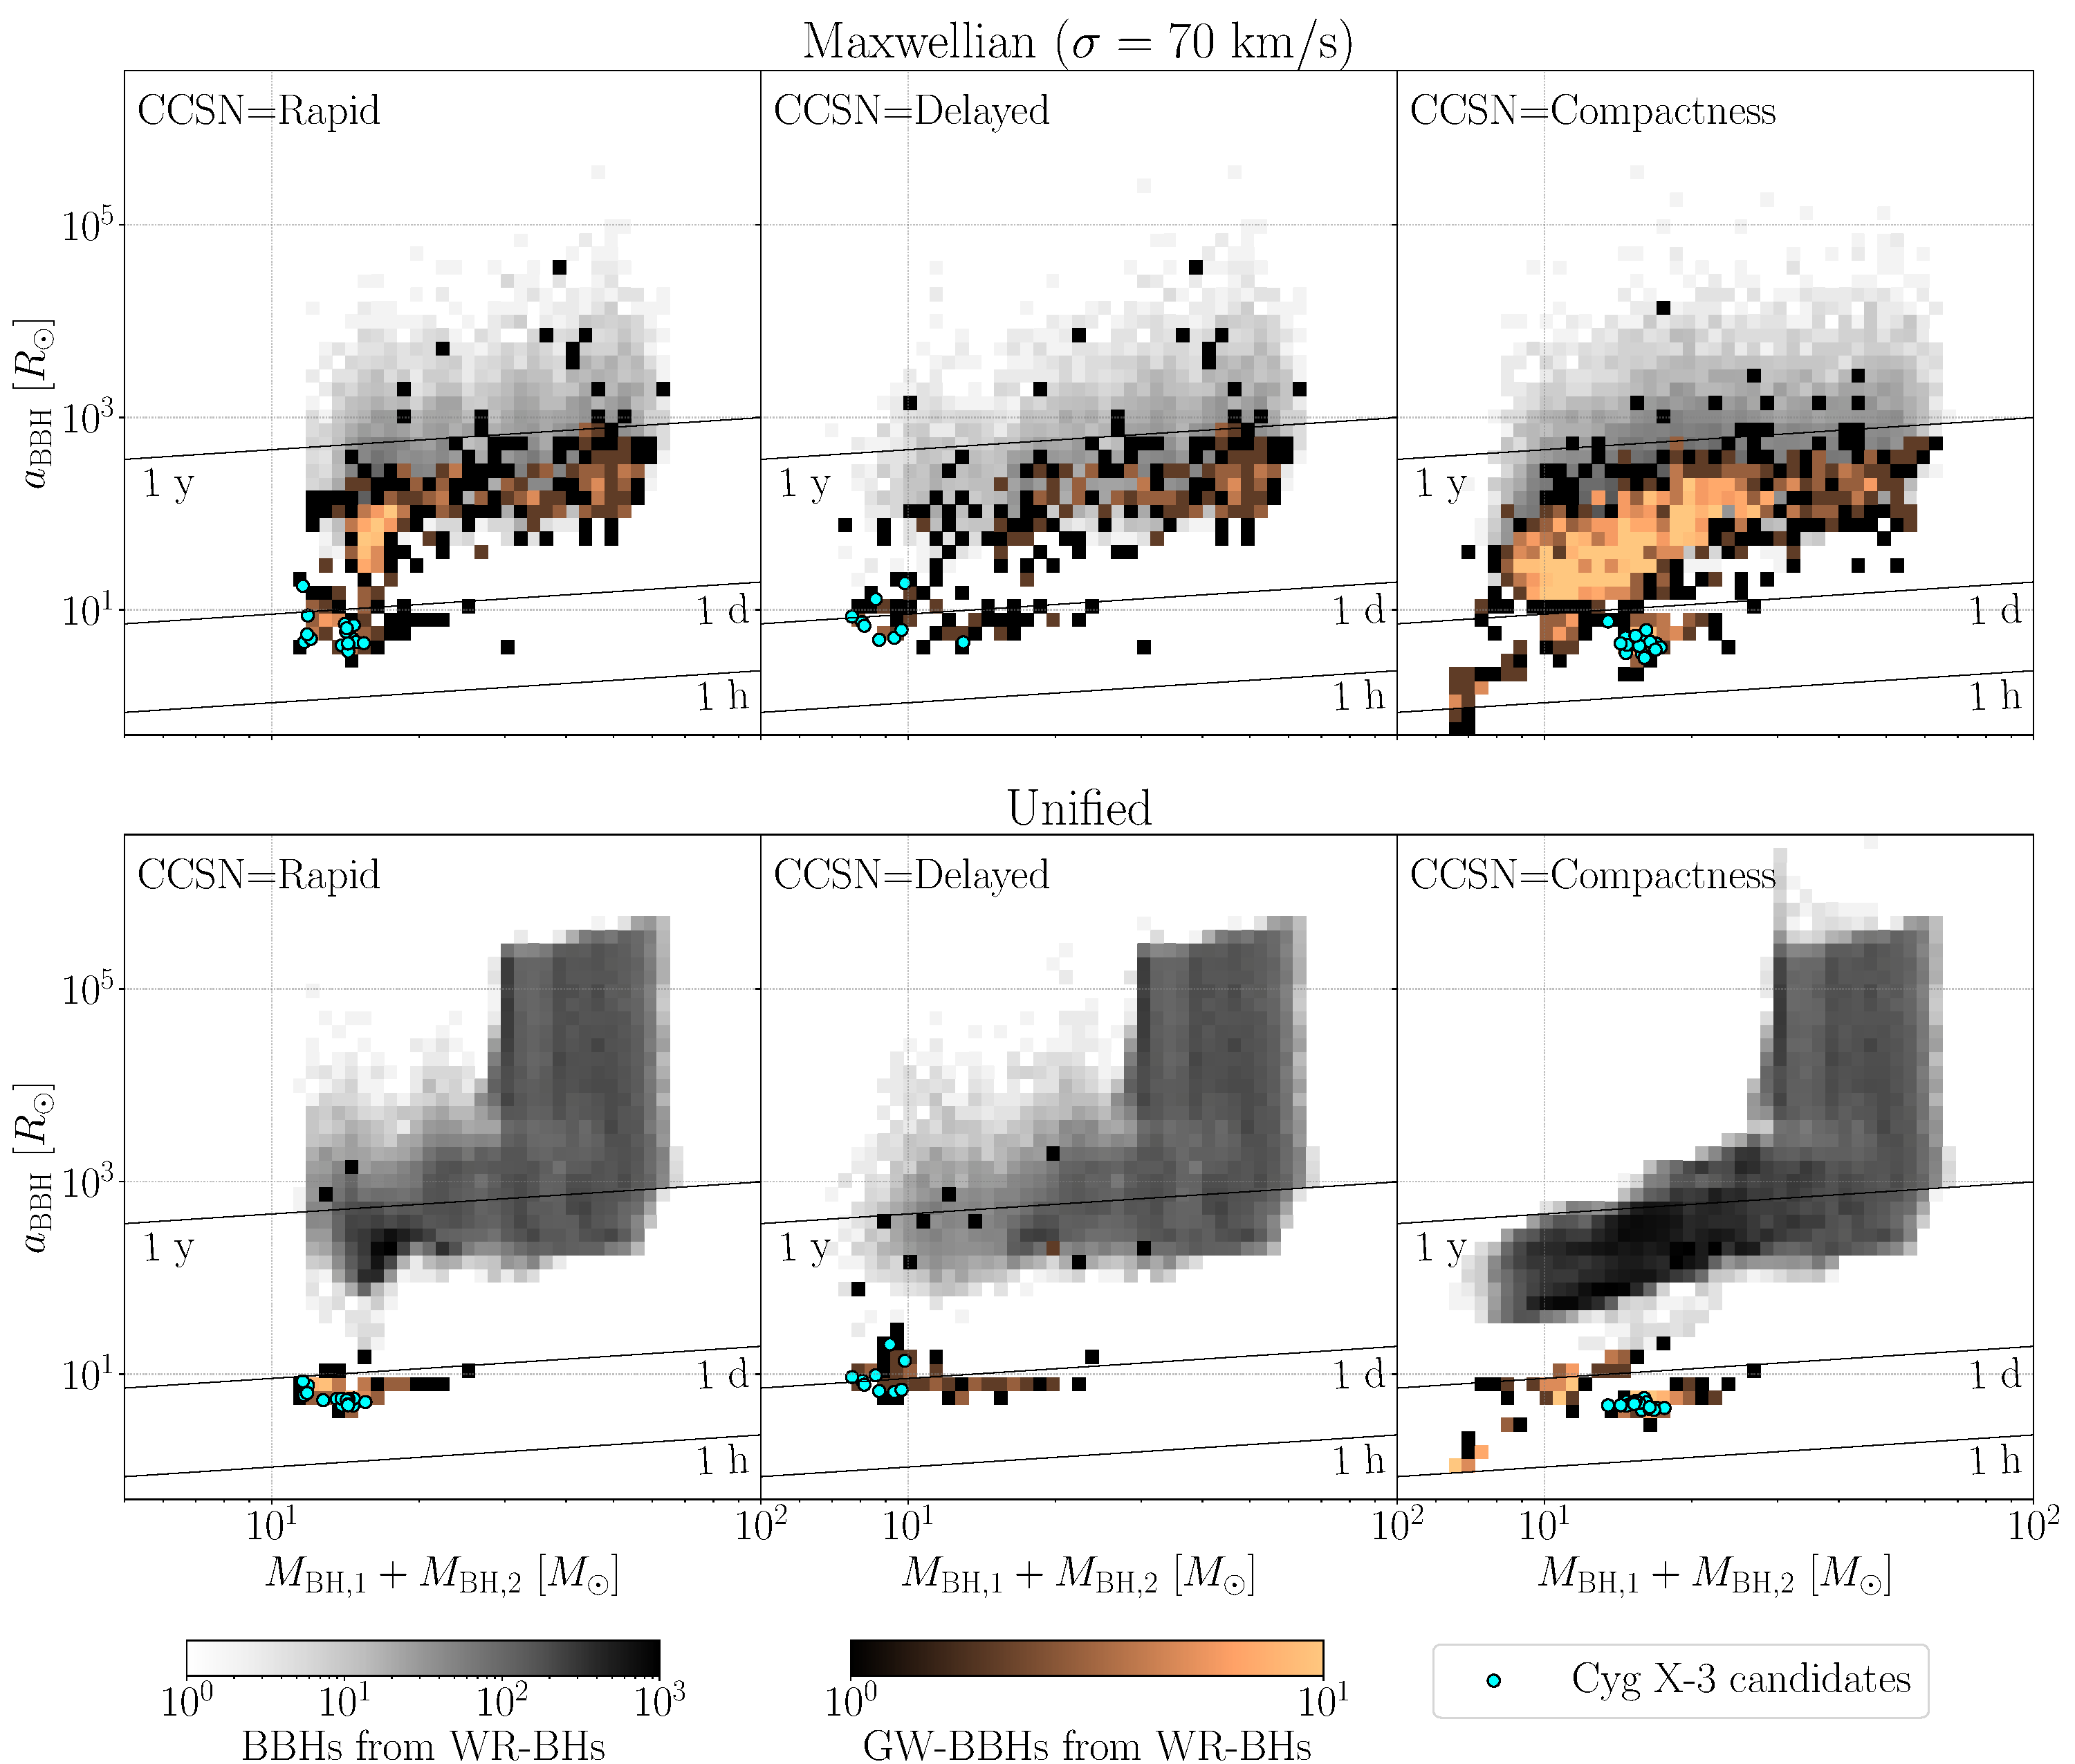
\includegraphics[width=\textwidth]{./images/kickcompare_rem_015_beamer.pdf}
		\end{column}
		\begin{column}{0.25\textwidth}
			\scriptsize
			\centering
			\evidenzia{\textbf{Natal kicks}}\\
			\bigskip
			\textbf{Pure Maxwellian}\\
			$\downarrow$\\
			merging BBHs \\$a_{\text{BBH}} \lesssim 1000~R_\odot$\\
			$\uparrow$\\
			$t_{\text{GW}} \propto (1-e^2)^{7/2}$\\
			\referenza{Peters 1964}\\
			\bigskip
			\smallskip
			\textbf{Maxwellian \\ rescaled} for \\
			\begin{itemize}
				\item Compact object mass
				\item Ejecta mass
			\end{itemize}
		$\downarrow$\\
		merging BBHs \\$a_{\text{BBH}} \lesssim 20~R_\odot$
		\vspace{.5cm}
		\end{column}	
	\end{columns}
	
\end{frame}



\begin{frame}{Probing the parameter space at Z=0.02}
	\begin{columns}
		\begin{column}{0.9\textwidth}
			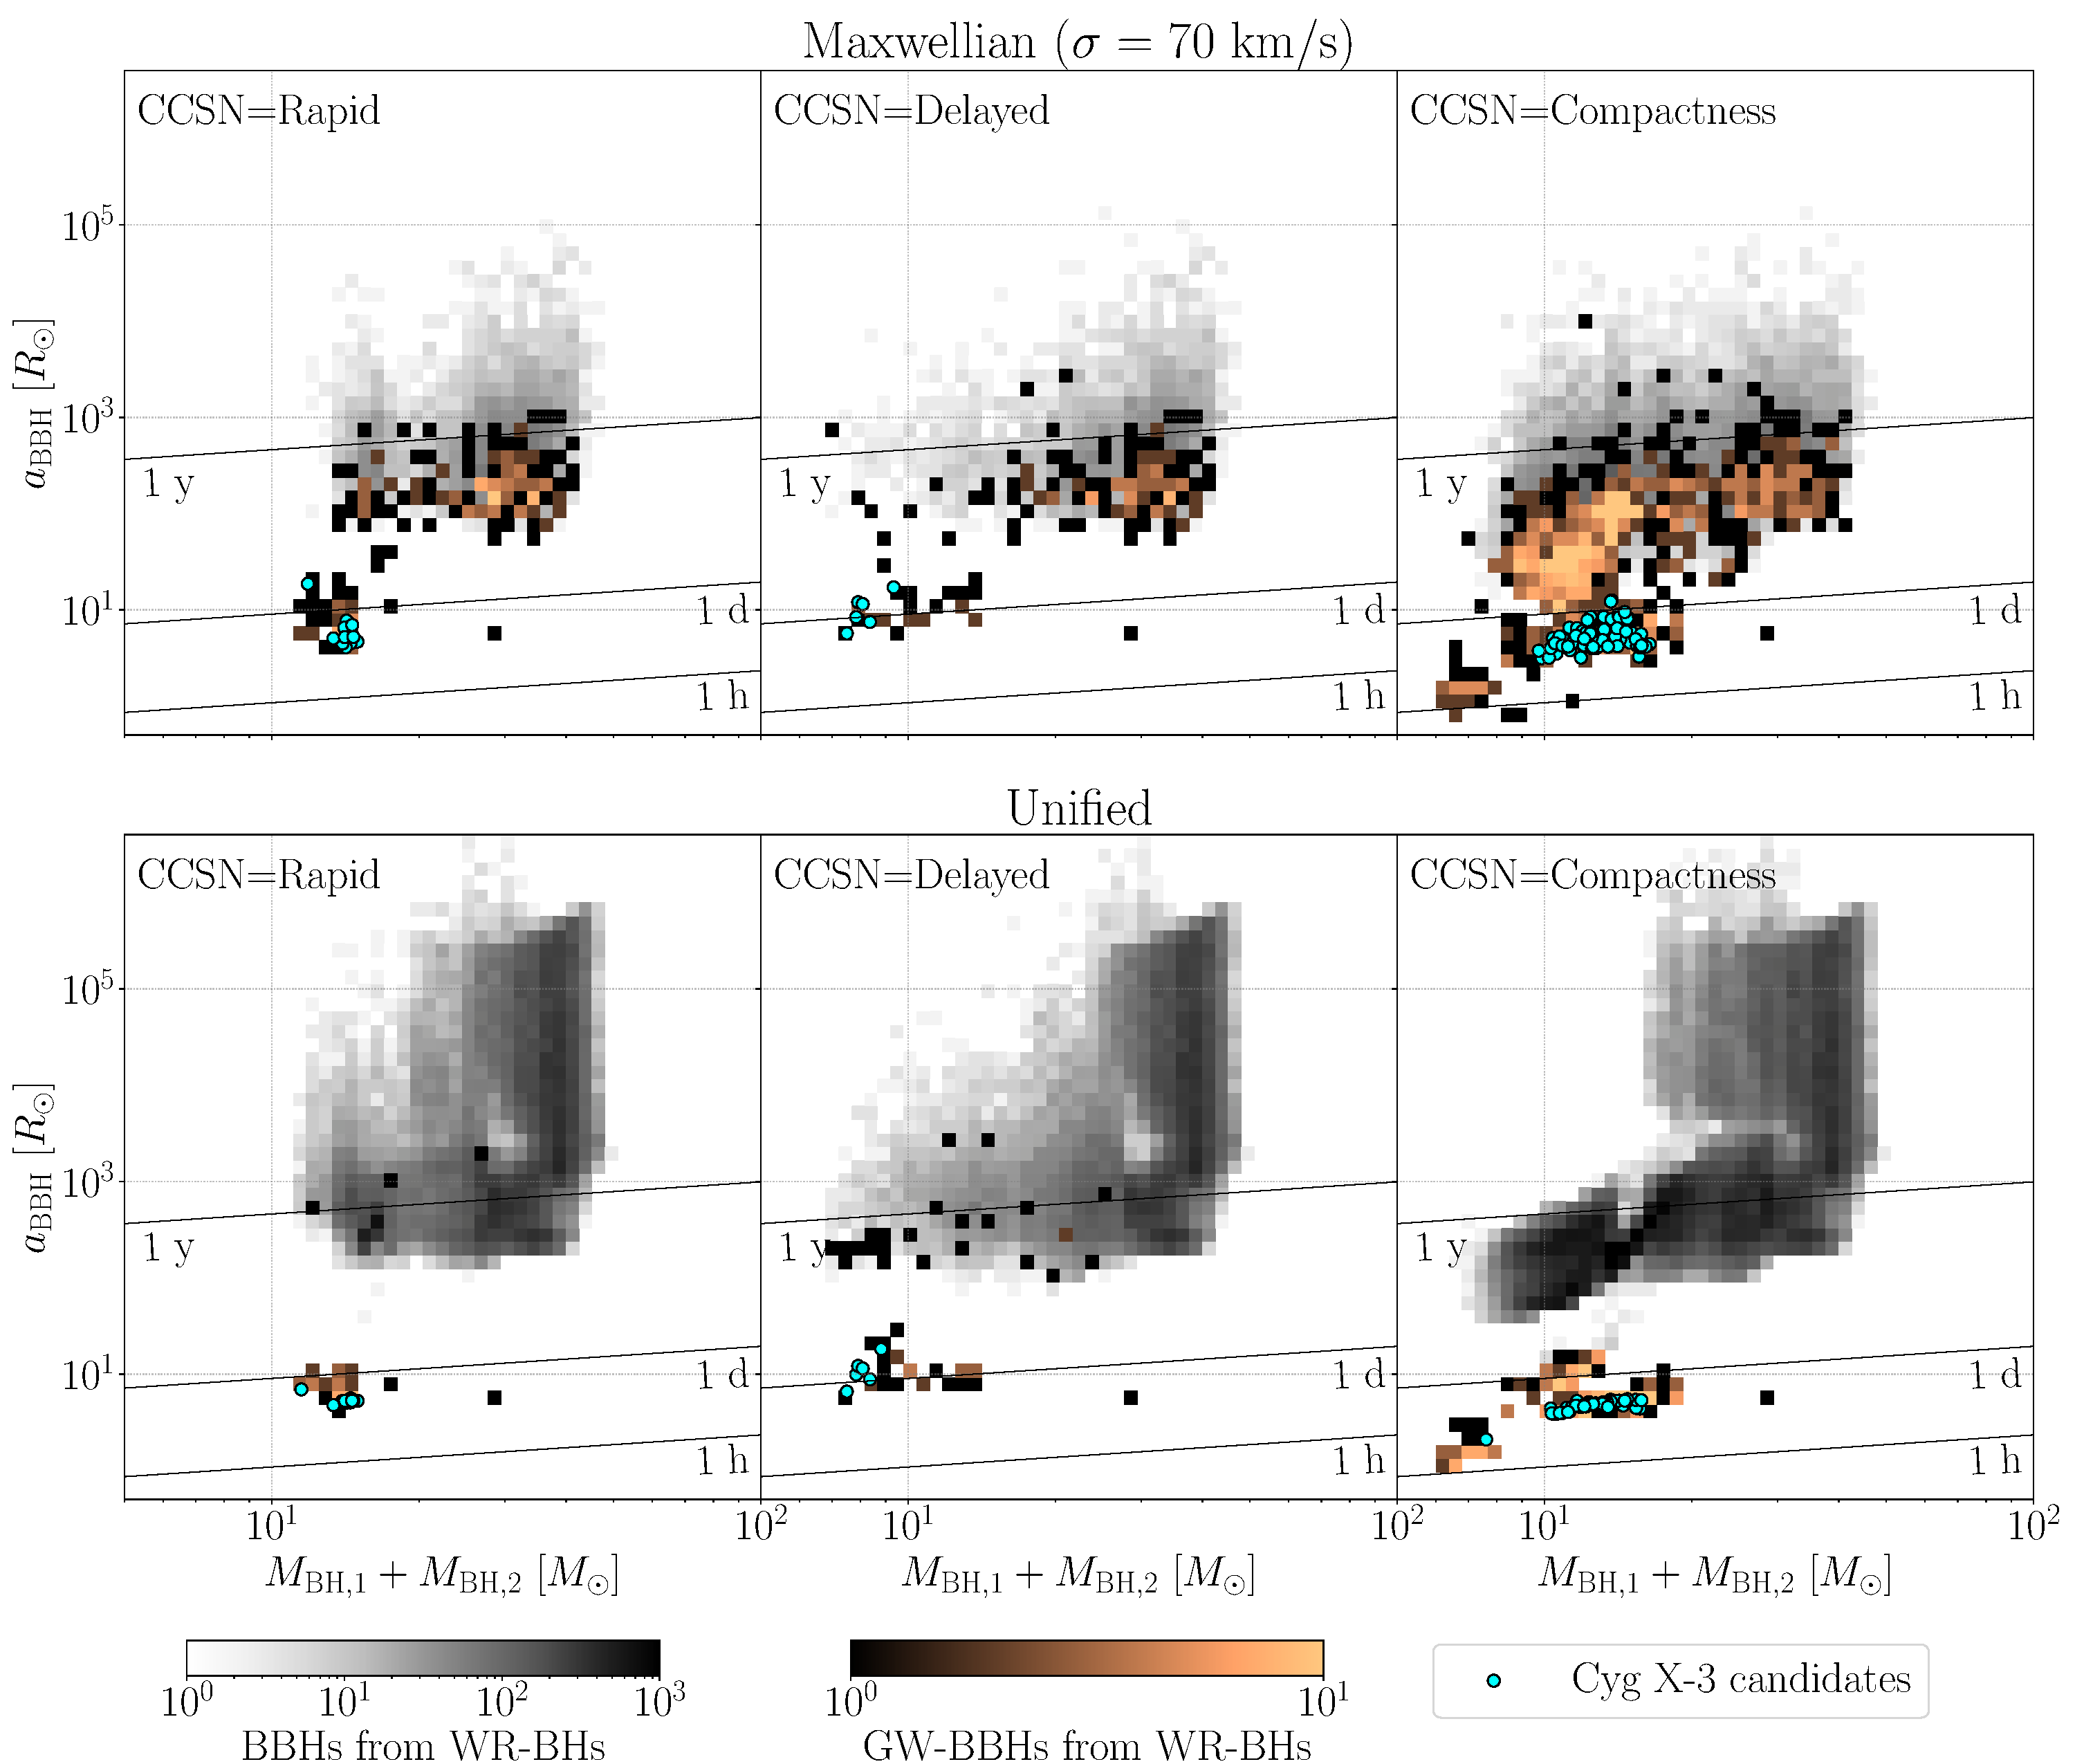
\includegraphics[width=\textwidth]{./images/kickcompare_rem_02_beamer.pdf}
		\end{column}
		\begin{column}{0.25\textwidth}
			\scriptsize
			\centering
			\evidenzia{\textbf{Metallicity}}\\
			\bigskip
			\textbf{Negligible effect}\\
			\bigskip
			$\uparrow$ \\
			\bigskip
			Mass variation \\
			\bigskip
			$\downarrow$\\
			\bigskip
			\textbf{Mass transfer \\ selection}\\
			\bigskip
			\evidenzia{\textbf{CCSN}}
		\end{column}	
	\end{columns}
	
\end{frame}




\begin{frame}{Delayed CCSN: 2 common envelope}
	\begin{columns}
		\begin{column}{0.22\textwidth}
			\tiny
			\centering
			\def\svgwidth{.9\textwidth}
			\import{./images/}{Delayed.pdf_tex} 
		\end{column}
	\hspace{0.5cm}
		\begin{column}{0.3\textwidth}
			\Large
			\vspace{1.3cm}
			$\Biggl\}$ \small Mass transfer\\
			\vspace{0.4cm}
			\Large
			$~\Biggl\}$ \small Mass transfer\\
		\end{column}
		\begin{column}{0.5\textwidth}
			\centering
			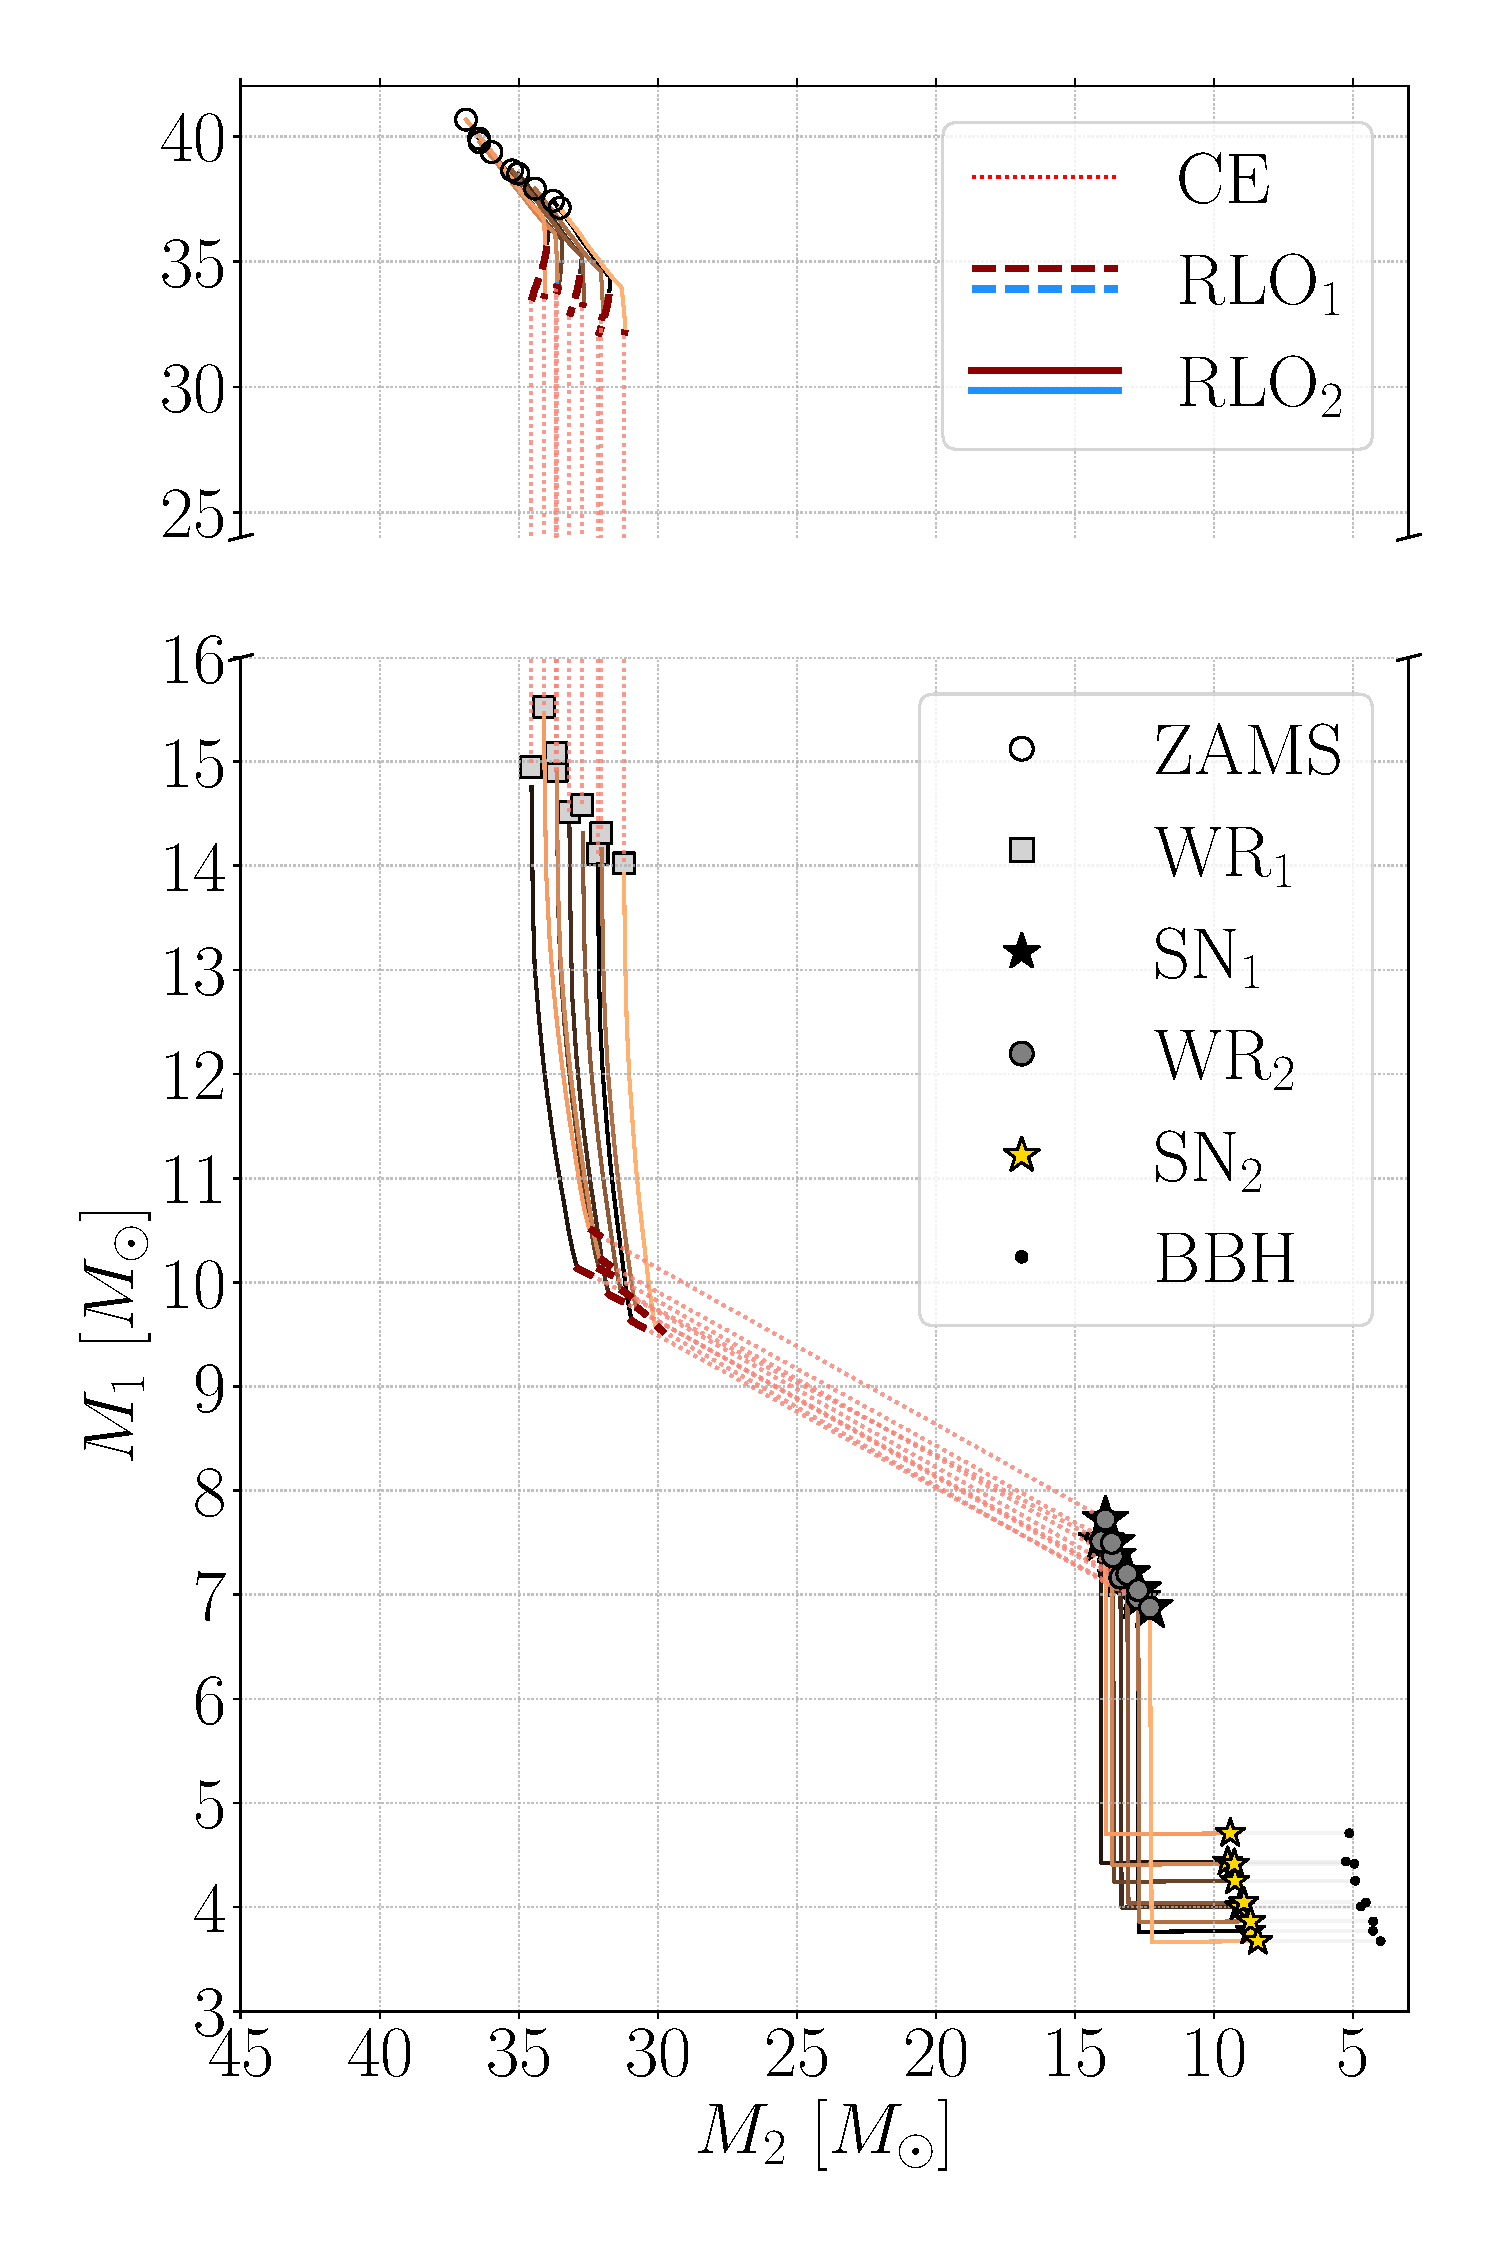
\includegraphics[width=\textwidth]{./images/del_Mass_1_Mass_0_BHBH_GW_WRBH_cyg_x-3--Ko17.pdf}
		\end{column}	
	\end{columns}
\end{frame}

\begin{frame}{Compactness CCSN: 2 or 3 mass transfer}
	\begin{columns}
		\begin{column}{0.5\textwidth}
			\tiny
			\def\svgwidth{1.2\textwidth}
			\import{./images/}{Compact.pdf_tex} 			
		\end{column}
		\hspace{1cm}
		\begin{column}{0.5\textwidth}
				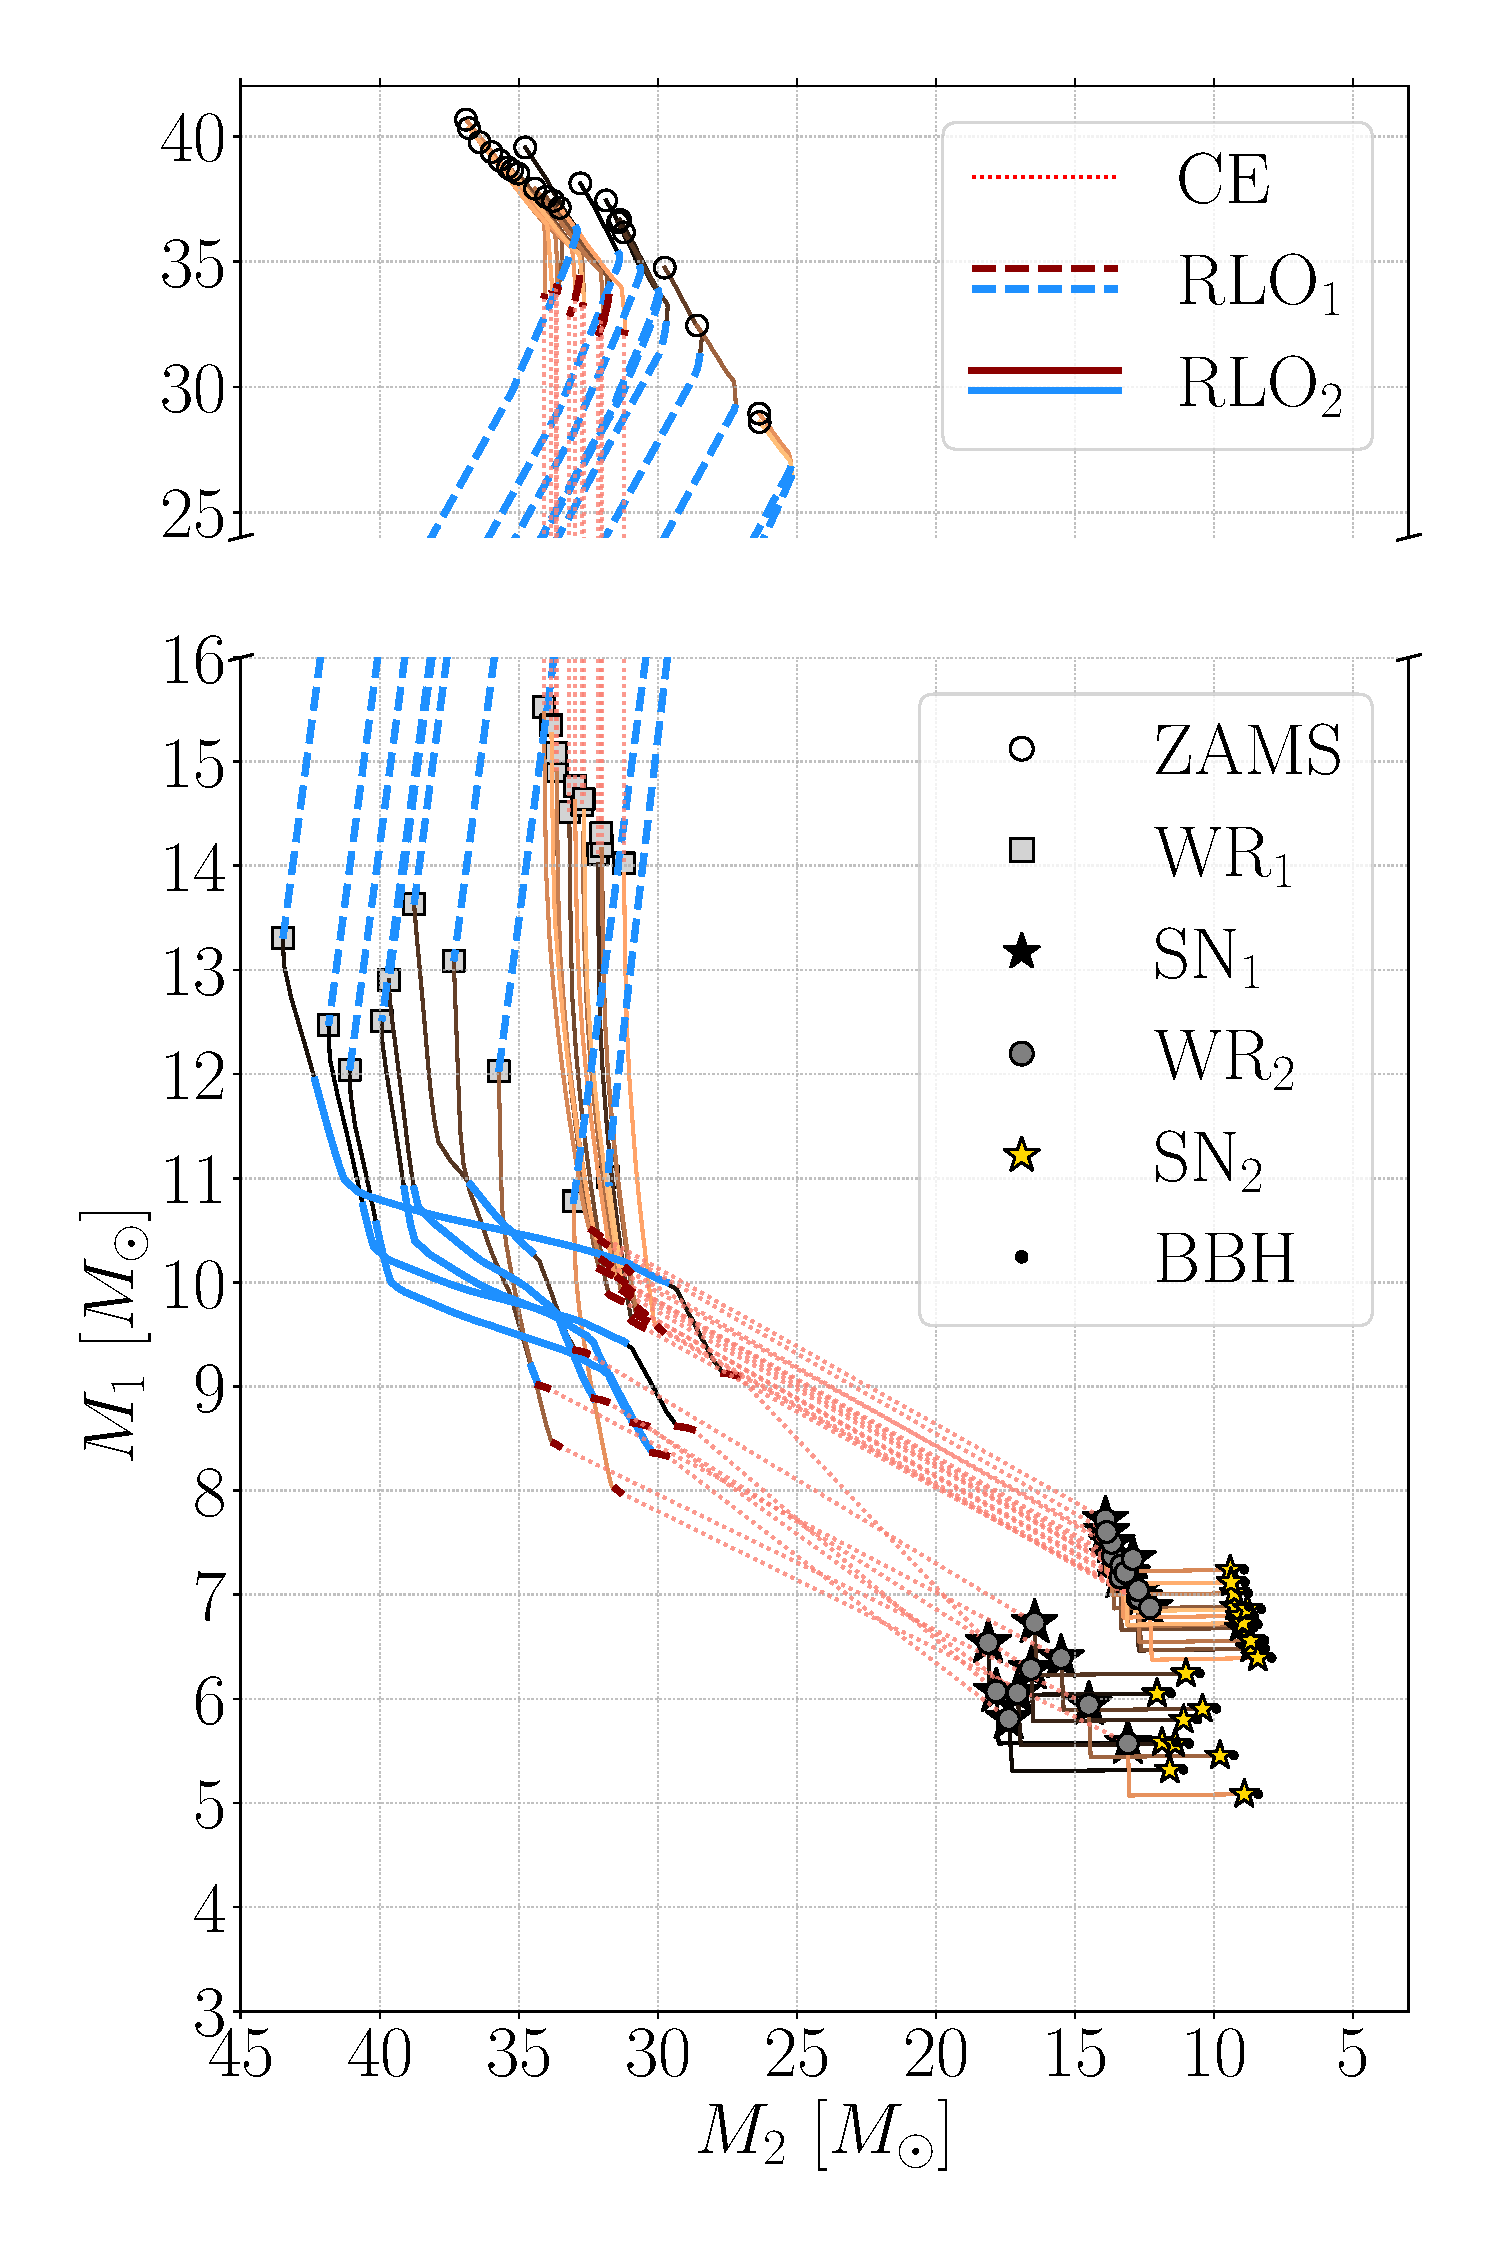
\includegraphics[width=\textwidth]{./images/com_Mass_1_Mass_0_BHBH_GW_WRBH_cyg_x-3--Ko17.pdf}
		\end{column}	
	\end{columns}
\end{frame}


\begin{frame}{Cyg X-3 evolution and properties}
	\scriptsize
	\begin{columns}
		\begin{column}{0.6\textwidth}
			\evidenzia{\textbf{For the fiducial model:}}
			\begin{itemize}
				\item $M_{\text{ZAMS,1,2}} \sim 30-40~M_\odot$\\
				$a_{\text{ZAMS}} \sim 50-3000~R_\odot$
				\item 2 or 3 mass transfer episodes \\
				\textbf{(1 common envelope needed)}
				\item Wolf-Rayet -- black hole for $\sim 0.5$ Myr
				\item \textbf{Wind-fed systems}
				\item BBHs merging in $\sim 50-200$ Myr
			\end{itemize}
		\bigskip
		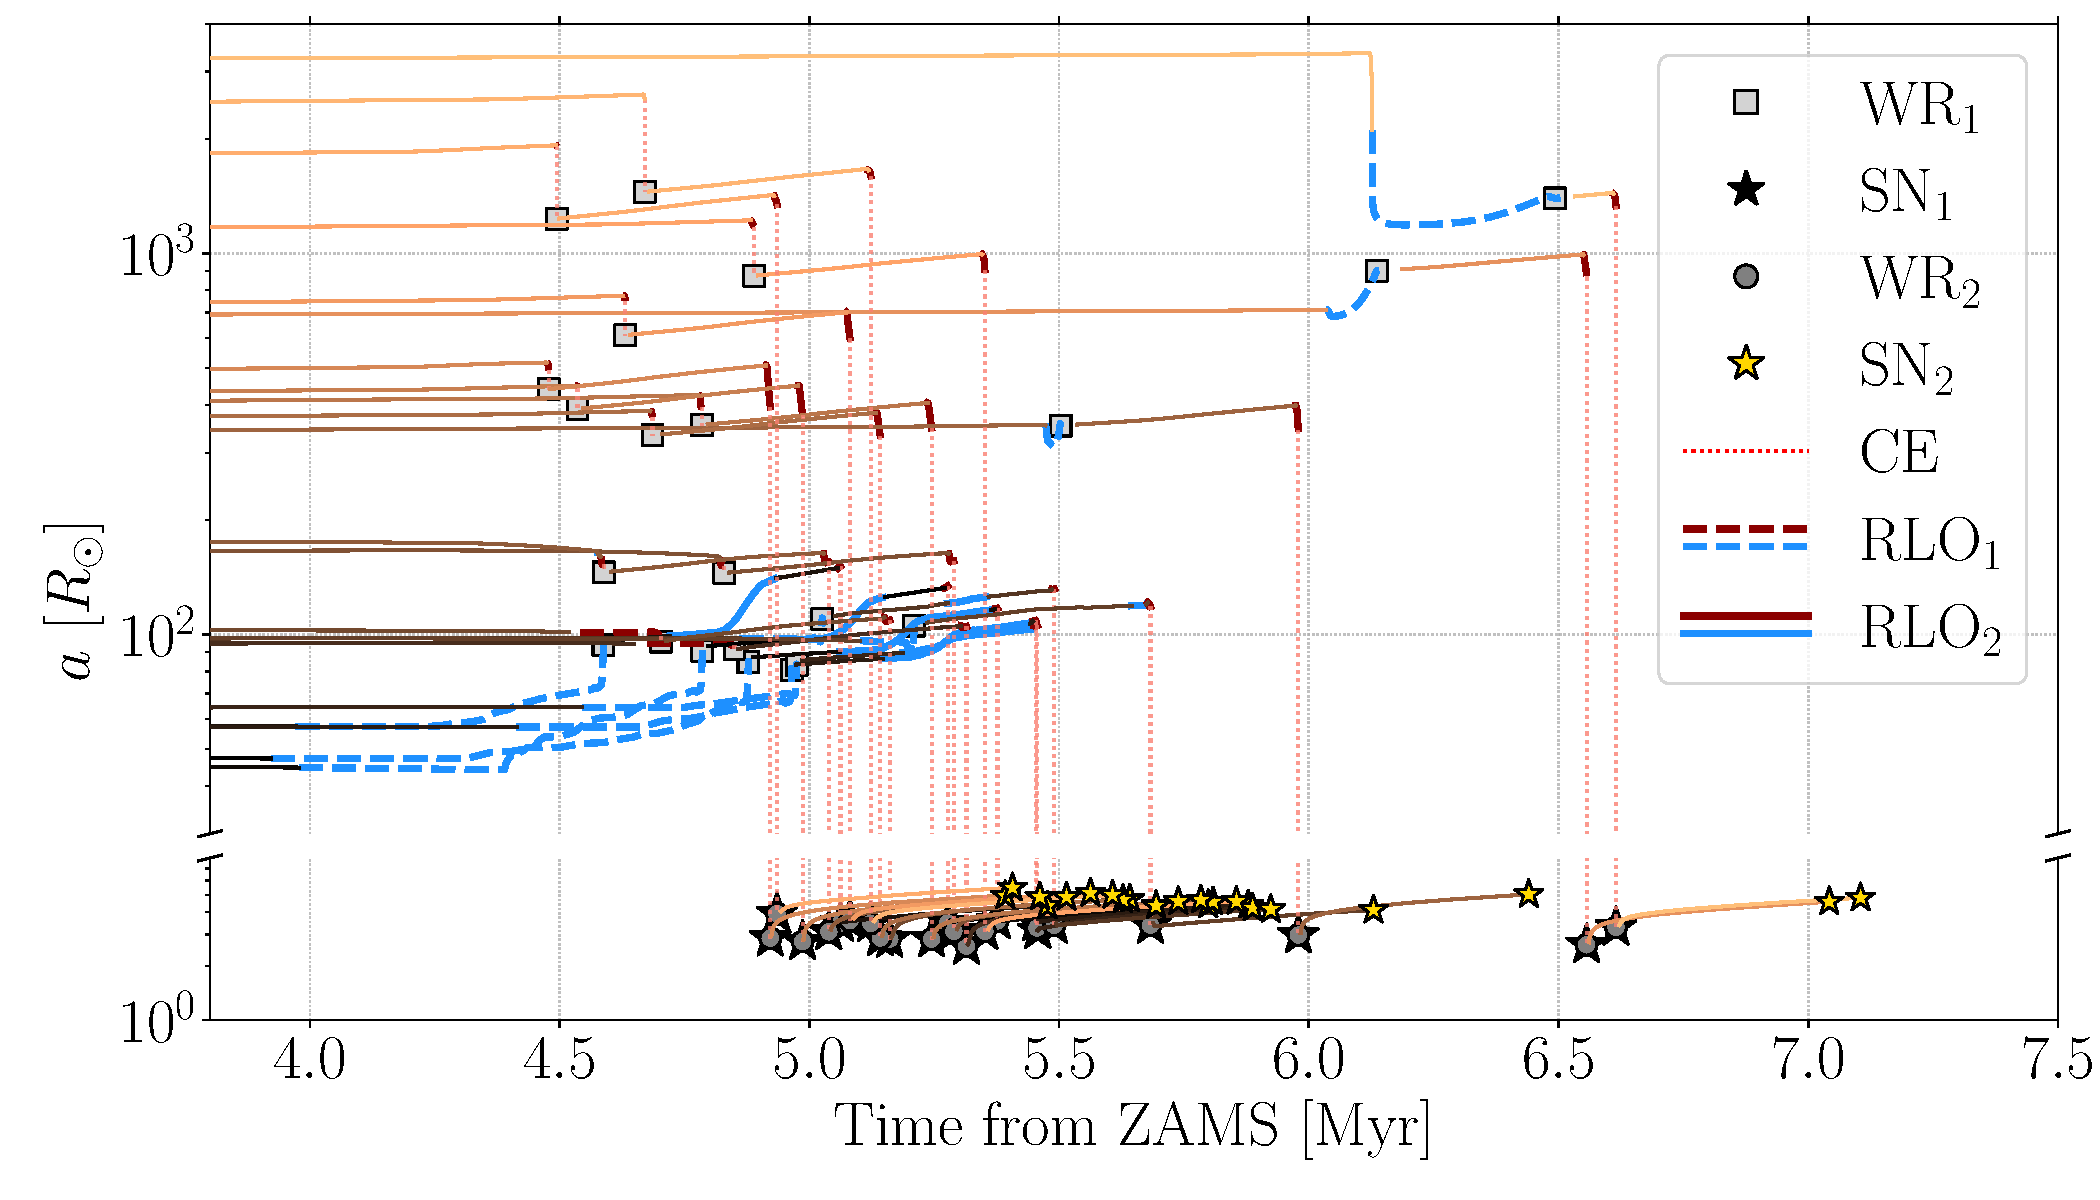
\includegraphics[width=\textwidth]{./images/BWorldtime_Semimajor_BHBH_GW_WRBH_cyg_x-3--Ko17.pdf}
		\end{column}
	
		\begin{column}{0.5\textwidth}
			\centering
			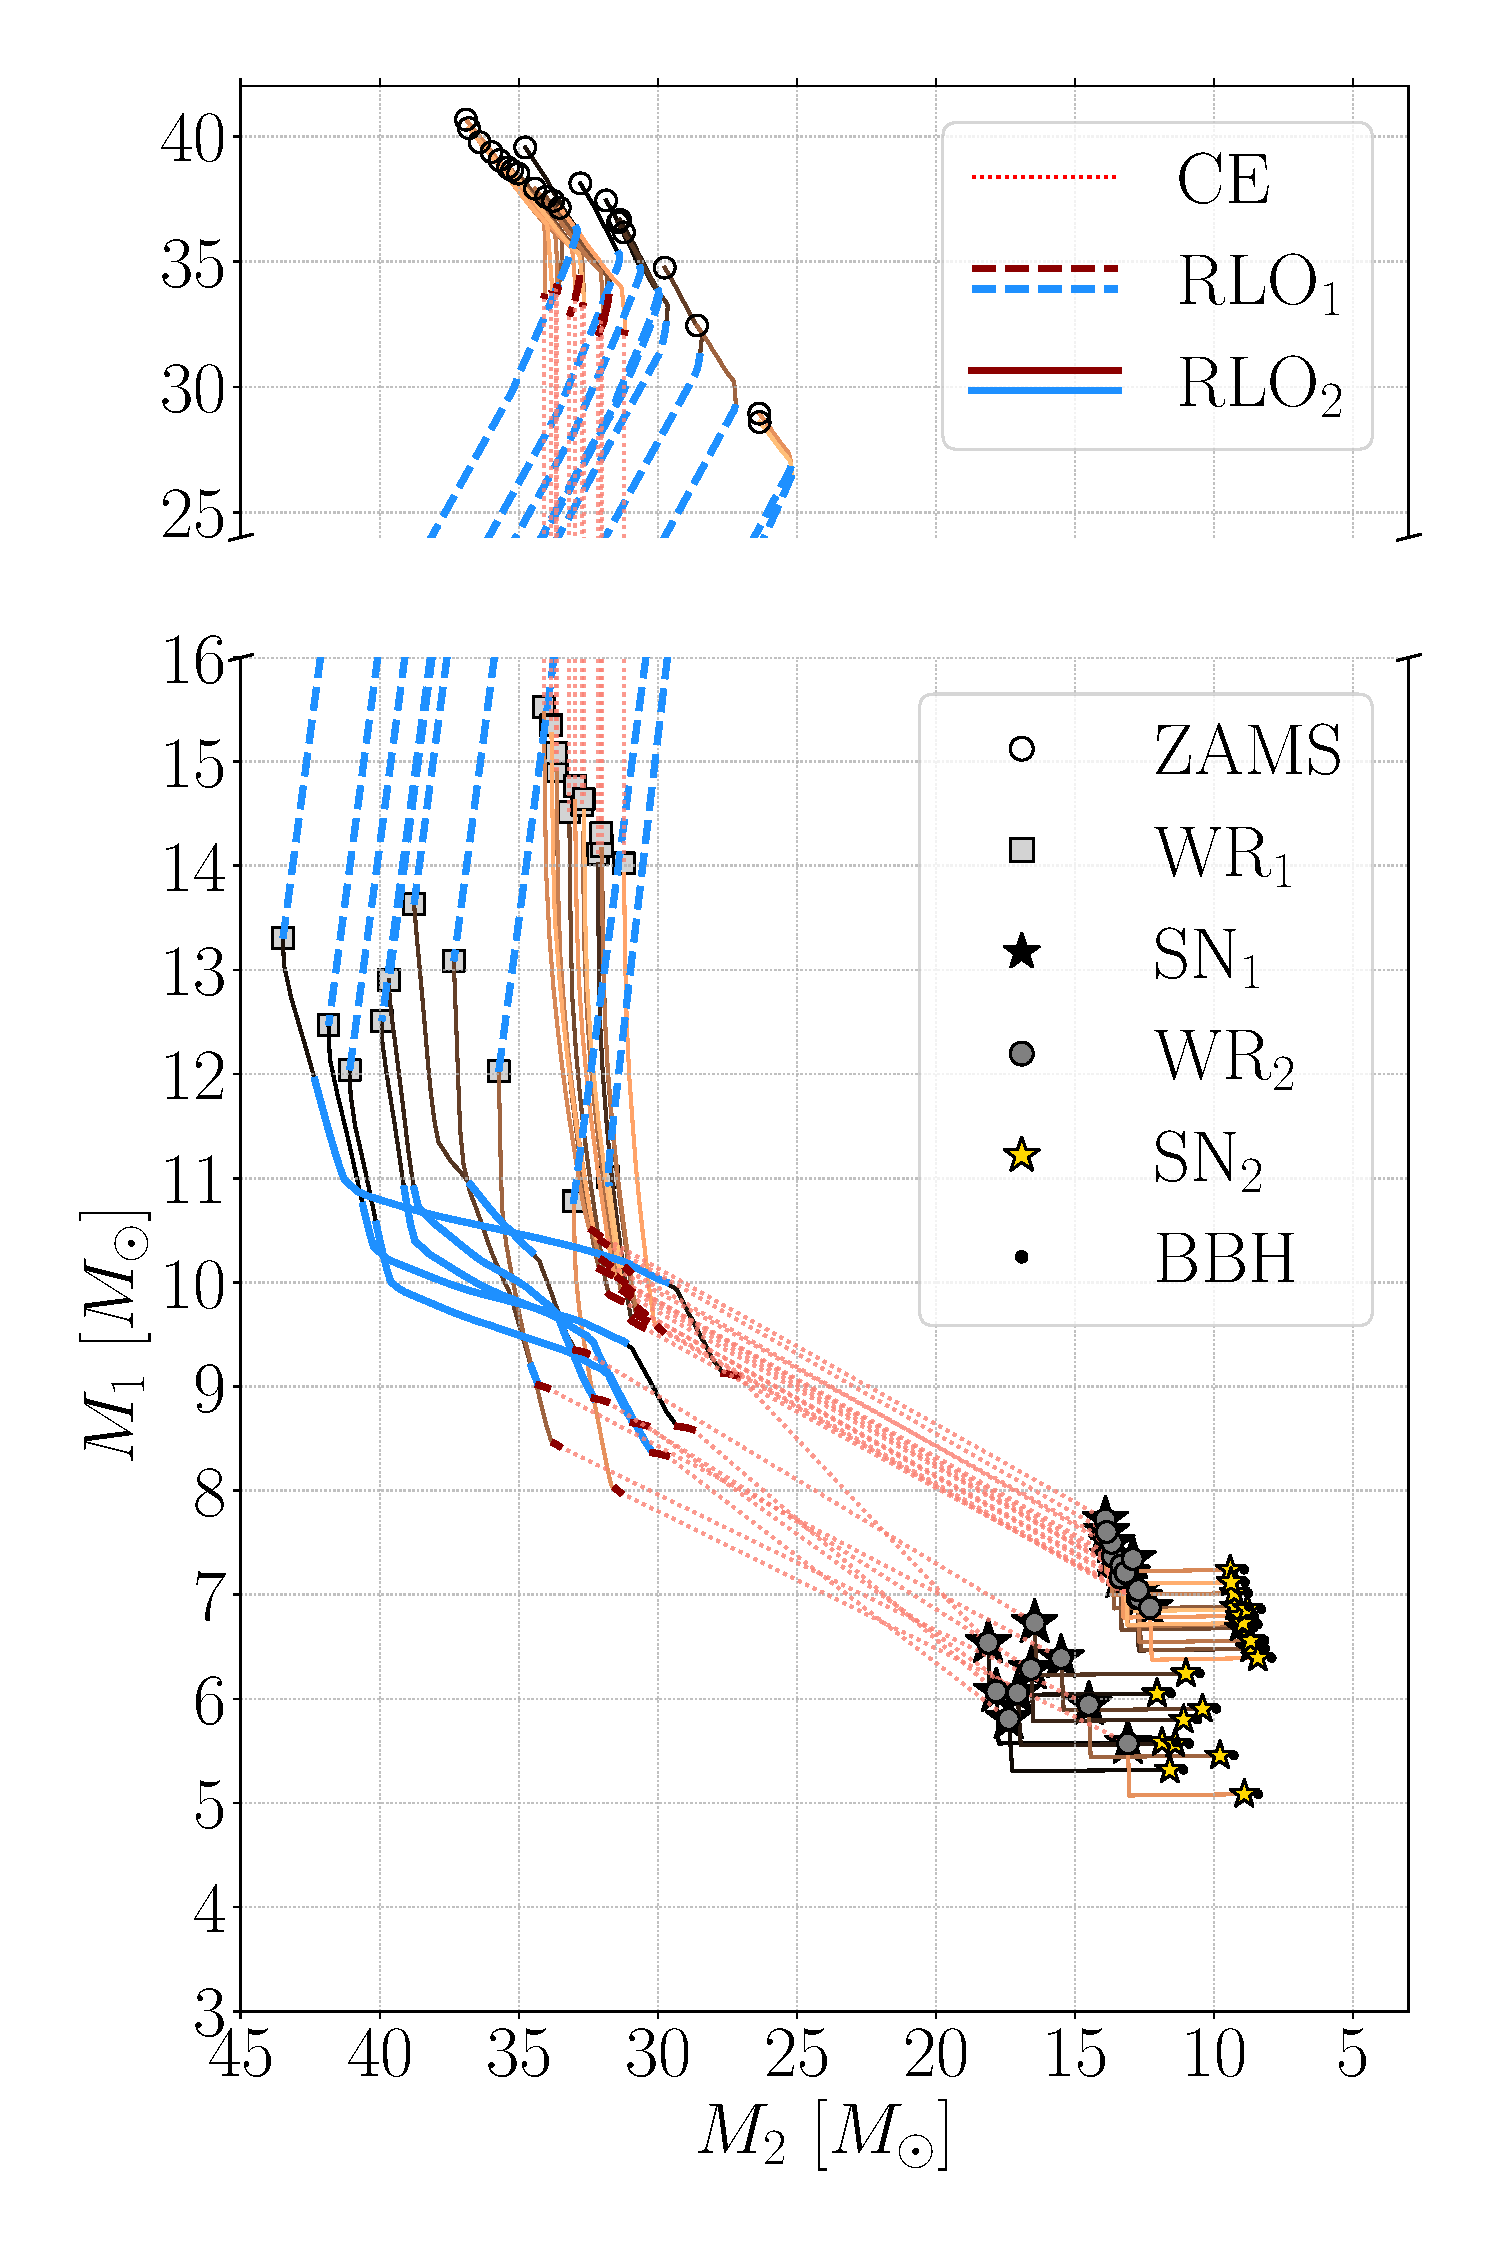
\includegraphics[width=\textwidth]{./images/com_Mass_1_Mass_0_BHBH_GW_WRBH_cyg_x-3--Ko17.pdf}
		\end{column}
	\end{columns}
\end{frame}

\begin{frame}{Conclusions}
	\scriptsize
	\begin{columns}
		\begin{column}{0.6\textwidth}
			\evidenzia{\textbf{Results (almost) model-independent:}}
			\begin{enumerate}
				\item Wolf-Rayet -- black hole: necessary stage \\ to form merging BBHs at $\boldsymbol{Z_\odot}$ \\
				($\bm{\gtrsim} \textbf{90}\%$ \textbf{probability}) 
				\item Cyg X-3: progenitor of merging BBHs ($\bm{\gtrsim} \textbf{75}\%$ \textbf{probability}) 
			\end{enumerate}	
			\bigskip	
			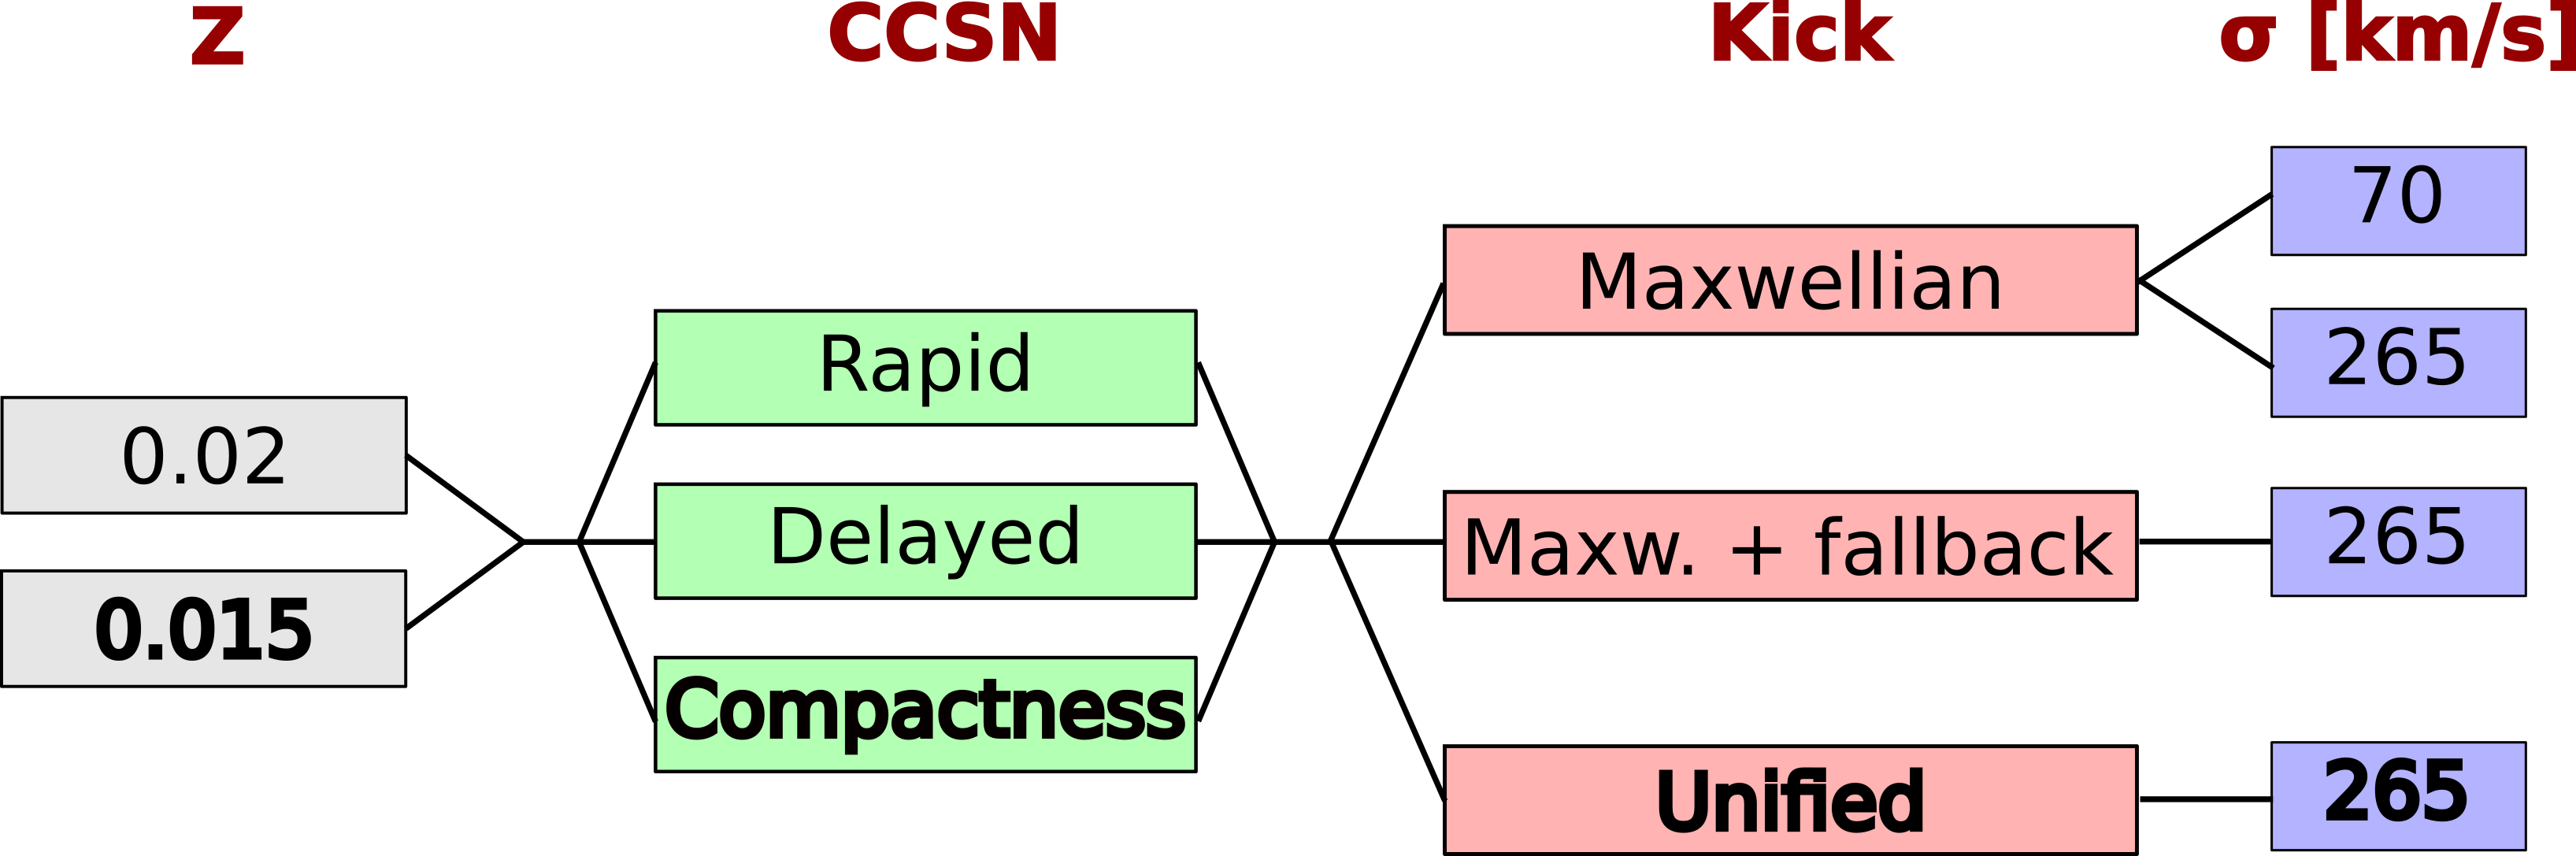
\includegraphics[width=\textwidth]{./images/parameterspace.png}
		\end{column}
		\begin{column}{0.5\textwidth}
			\evidenzia{\textbf{Cyg X-3:}}\\
			\begin{itemize}
				\item \textbf{Representative} of a \textbf{sub-population of merging BBHs progenitors}
				\item 2 or 3 mass transfer \\(\textbf{1 common envelope})
			\end{itemize}
			\smallskip
			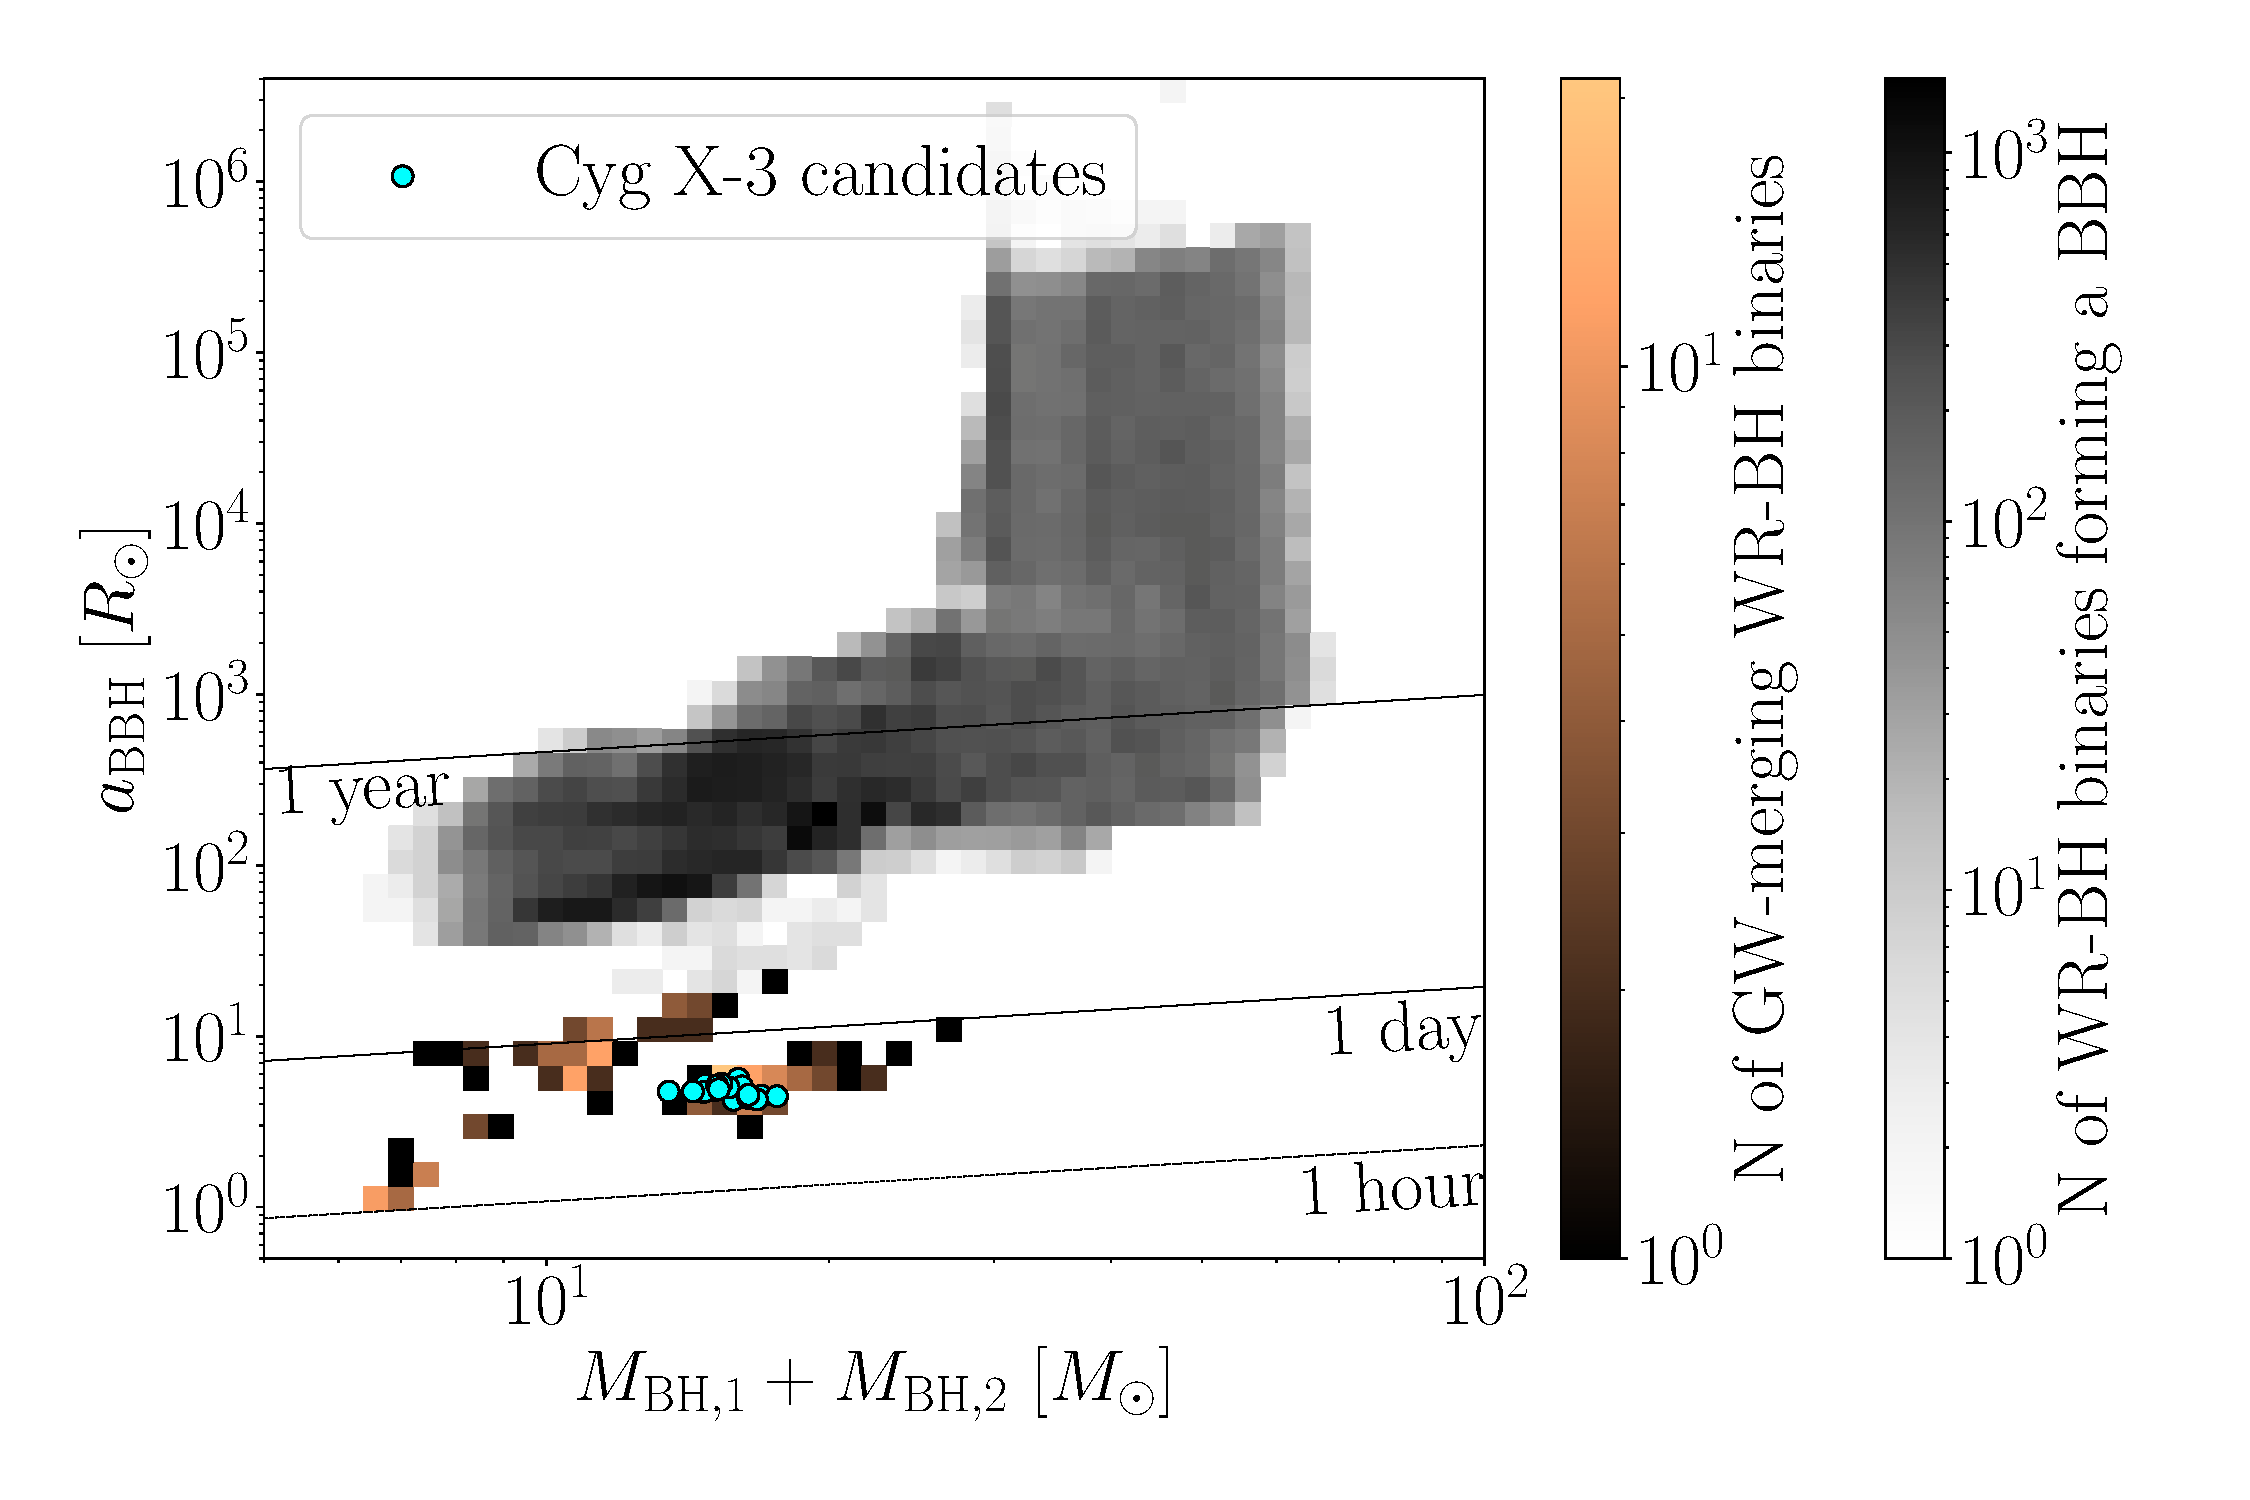
\includegraphics[width=\textwidth]{./images/avsMtotREMBHBH_GW_WRBH_BHBH_GW_WRBH_cyg_x-3--Ko17.pdf}			
			\vspace{-1.1cm}
		\end{column}
	\end{columns}
	\bigskip
	\bigskip
	\centering
	\textbf{Wolf-Rayet -- black hole observations $\rightarrow$ ``Rosetta stone'' for merging BBHs}\\
	\bigskip
	\small
	\evidenzia{\textbf{Thank you for the attention}}
	
\end{frame}



%%%%%%%%%%%%%%%%%%%%%%%%%%%%%%%%%
%%%%%%% extra slides %%%%%%%%%%%%
%%%%%%%%%%%%%%%%%%%%%%%%%%%%%%%%%

\begin{frame}[noframenumbering]
	\centering
	\Large
	\evidenzia{\textbf{Additional slides}}
\end{frame}








\begin{frame}[noframenumbering]{CCSN models in \texttt{SEVN}}
	\small
	\begin{columns}
		\begin{column}{0.4\textwidth}
		\evidenzia{\textbf{Rapid}}\\
		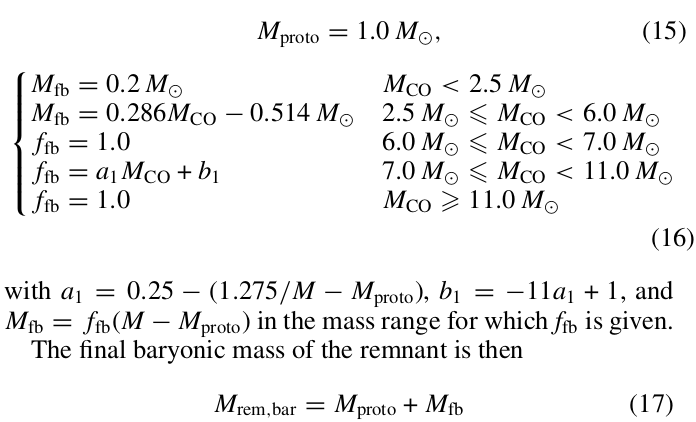
\includegraphics[width=\textwidth]{./images/rapid.png}\\
		\evidenzia{\textbf{Delayed}}\\
		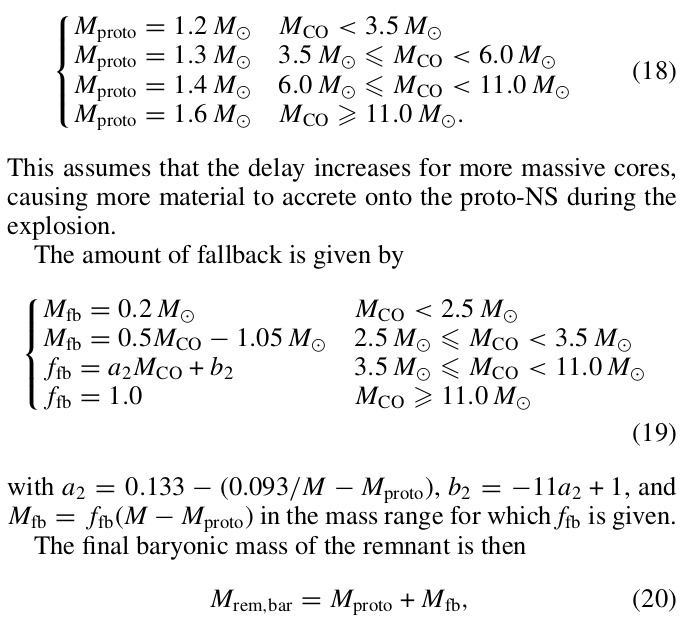
\includegraphics[width=\textwidth]{./images/delayed.png}\\
		\referenza{Fryer et al. 2012}
		\end{column}
		\begin{column}{0.5\textwidth}
		\evidenzia{\textbf{Compactness}}\\
		$\xi_\mathrm{2.5}= \frac{2.5}{R(2.5 ~M_\odot)}$\\
		\referenza{O'Connor et al. 2011}\\
		\medskip
		$\xi_{2.5} = 0.55 -1.1 \left(\frac{1~ M_\odot}{M_{\rm CO}}\right)$\\
		\referenza{Mapelli et al. 2020}\\
		\medskip
		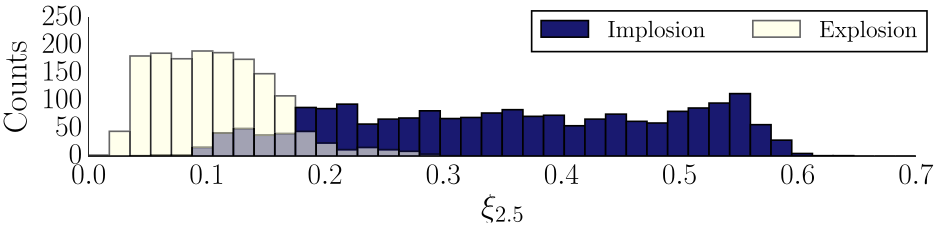
\includegraphics[width=\textwidth]{./images/compactness.png}\\
		\referenza{Sukhbold et al. 2016}\\
		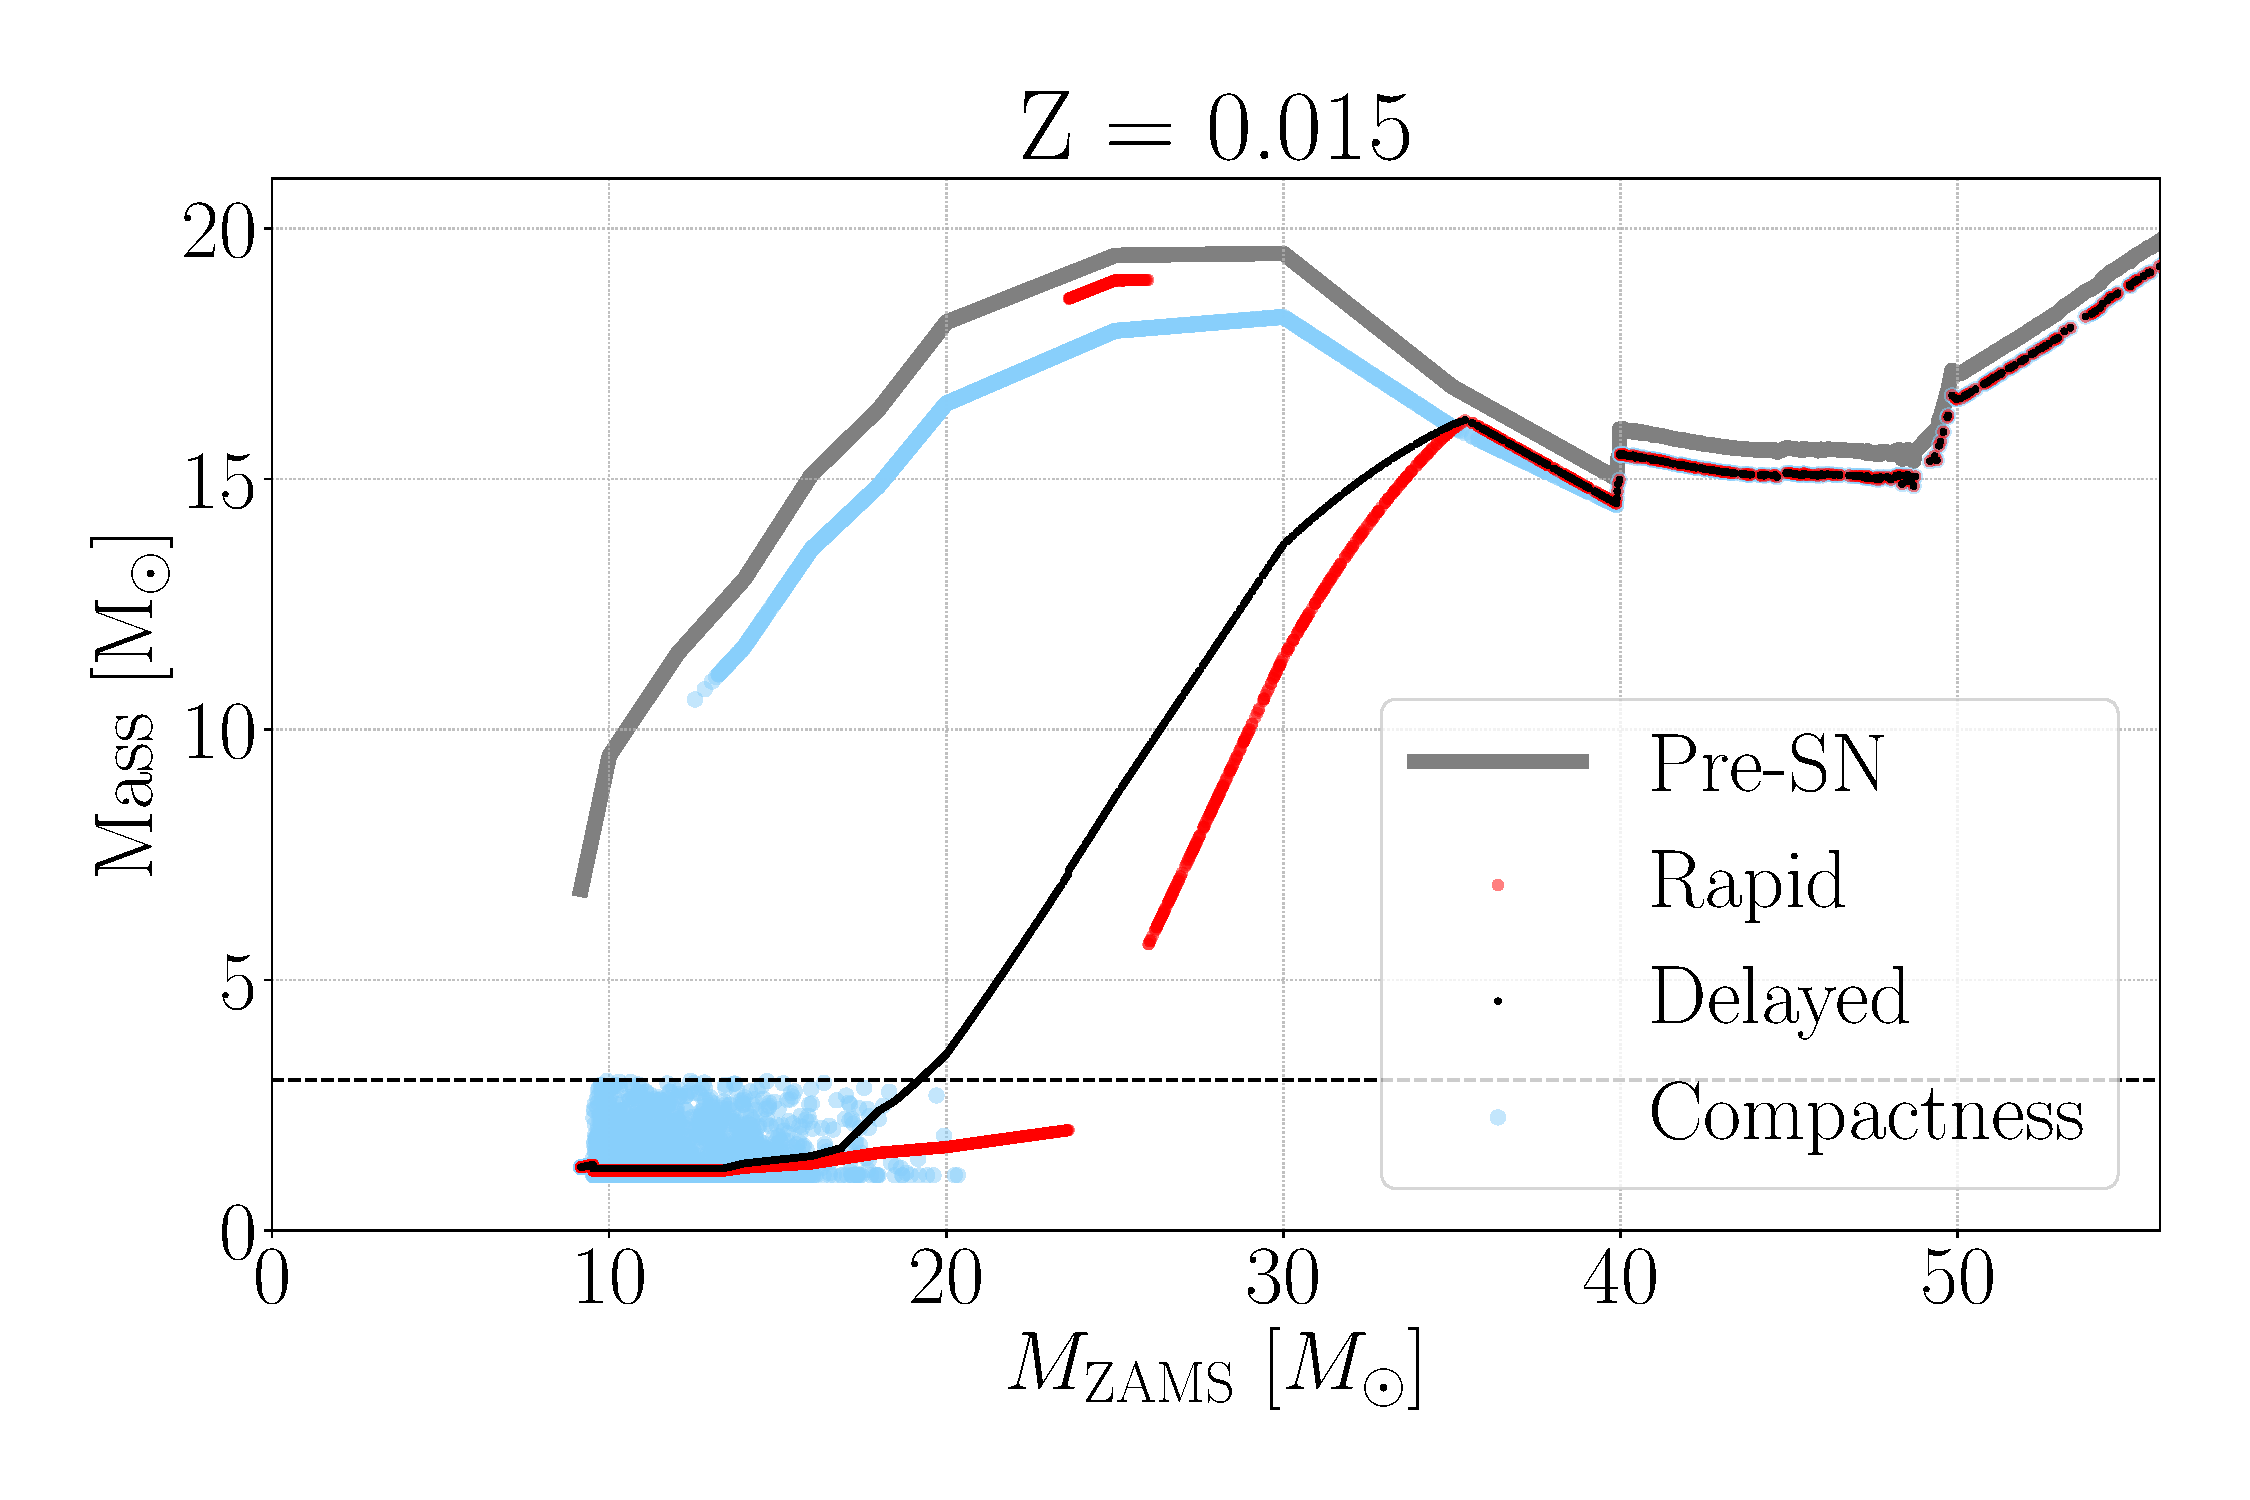
\includegraphics[width=\textwidth]{./images/remnants_Z015_cut.pdf}
		\end{column}	
	\end{columns}
\end{frame}


\begin{frame}[noframenumbering]{Kick models in \texttt{SEVN}}
		\small
		\evidenzia{\textbf{Maxwellian}} \\
		\smallskip
		$\boxed{v = f_{\sigma}}$ \\
		\begin{itemize}
			\item $\sigma = 70$ km/s $\rightarrow$ BBHs natal kicks \\ \referenza{Atri et al. 2019}
			\item $\sigma = 265$ km/s $\rightarrow$ young pulsars natal kicks \\ \referenza{Hobbs et al. 2005}
		\end{itemize}
		\smallskip
		\evidenzia{\textbf{Maxwellian (+ fallback)}} \\
		\smallskip
		$\boxed{v = f_\sigma\,{} (1-f_{\rm fb})} \qquad \qquad f_{\rm fb}=M_{\rm fb}/(M_{\rm rem} - M_{\rm proto}) \in [0,1]$\\
		\referenza{Fryer et al. 2012}\\
		\medskip
		\evidenzia{\textbf{Unified}} \\
		\smallskip
		$\boxed{v = f_{\sigma} \frac{M_{\rm ej}}{\langle M_{\rm ej}\rangle} \frac{\langle M_{\rm NS}\rangle}{M_{\rm rem}}} \qquad ~~ M_{\rm ej} = M_{\rm pre-SN} - M_{\rm rem} $ \\ 
		\bigskip
		with $\langle M_{\rm NS}\rangle \sim 1.30~M_\odot \quad \langle M_{\rm ej}\rangle \sim 10.30 ~ M_\odot$ 
		\referenza{Giacobbo \& Mapelli 2020}
\end{frame}



\begin{frame}[noframenumbering]{Mass transfer in \texttt{SEVN}}
	\small
	\centering
	\evidenzia{Unstable Roche lobe overflow if $q \geq q_{\rm crit}$}\\
	\scriptsize
	\bigskip
	\bigskip
	    \begin{tabular}{lllcc}
		\toprule
		Stellar phase & Burning &  Condition & \texttt{BSE} phase &  $q_{\rm crit}$ \\ 
		\midrule
		Main sequence           & H-core       & $M_{\text{ZAMS}} \geq 0.7~M_\odot$          &  1  & 3.0        \\
		Hertzsprung-gap         & H-shell    & $f_{\rm conv} < 0.33$       &  2  & 4.0        \\
		First giant branch      & H-shell    & $f_{\rm conv} \geq 0.33$    &  3  & Equation \ref{eq:qcritgiants} \\
		Core He burning         & He-core     & $f_{\rm conv} < 0.33$       &  4  & 3.0 \\ 
		Asymptotic giant branch & He-shell    & $f_{\rm conv} \geq 0.33$    &  5  & Equation \ref{eq:qcritgiants} \\
		\hline
		Wolf-Rayet              & He-core     & $M_{\rm He} > 0.979~M$  &  7  & 3.0 \\ 
		Wolf-Rayet              & He-shell   & $M_{\rm He} > 0.979~M$  &  8  & 0.784 \\ 
		\bottomrule
	\end{tabular}
\bigskip
\bigskip
\begin{equation}\label{eq:qcritgiants}
q_\mathrm{crit} = 0.362 + \frac{1}{3\left(1-\frac{M_\mathrm{He,d}}{M_\mathrm{d}}\right)}.
\end{equation}
\referenza{Hurley et al. 2002, Iorio et al. in prep.}
\end{frame}

\begin{frame}[noframenumbering]{Initial conditions with \texttt{SEVN}}
	\scriptsize
		\begin{columns}
		\begin{column}{0.56\textwidth}
			\evidenzia{\textbf{Primary masses}}\acapo
			$\boxed{\xi(M_1) \propto M_1^{-2.3}} \qquad \qquad ~~ M_1 \in [10,150]~M_\odot$\\
			\referenza{Sana et al. 2012}\\
			\medskip
			\evidenzia{\textbf{Mass ratios}}\acapo
			
$\boxed{\xi(q) \propto q^{0.1}} \qquad \qquad \quad q=M_2/M_1 \in [0.1,1] $\\
\smallskip
$\xi(M_2) = \xi(M_1) \,{} \xi(q)  \qquad \qquad M_2 \in [1 ~M_\odot , M_1]$\\
\referenza{Sana et al. 2012}\\
\medskip
			\evidenzia{\textbf{Periods}}\acapo
			
$\boxed{\xi(\mathcal{P}) \propto \mathcal{P}^{-0.55}} ~~\mathcal{P} = \log(P/\text{days}) \in [0.30,5.5]$\\
\referenza{Sana et al. 2012}\\
\medskip
			\evidenzia{\textbf{Eccentricities}}\acapo
$\boxed{\xi (e (P)) \propto 1-(P/\text{days})^{-2/3}} \qquad P \geq 2~\text{days}$\\
\smallskip
\referenza{Moe \& Di Stefano 2017}
		
		\end{column}
		\begin{column}{0.6\textwidth}
				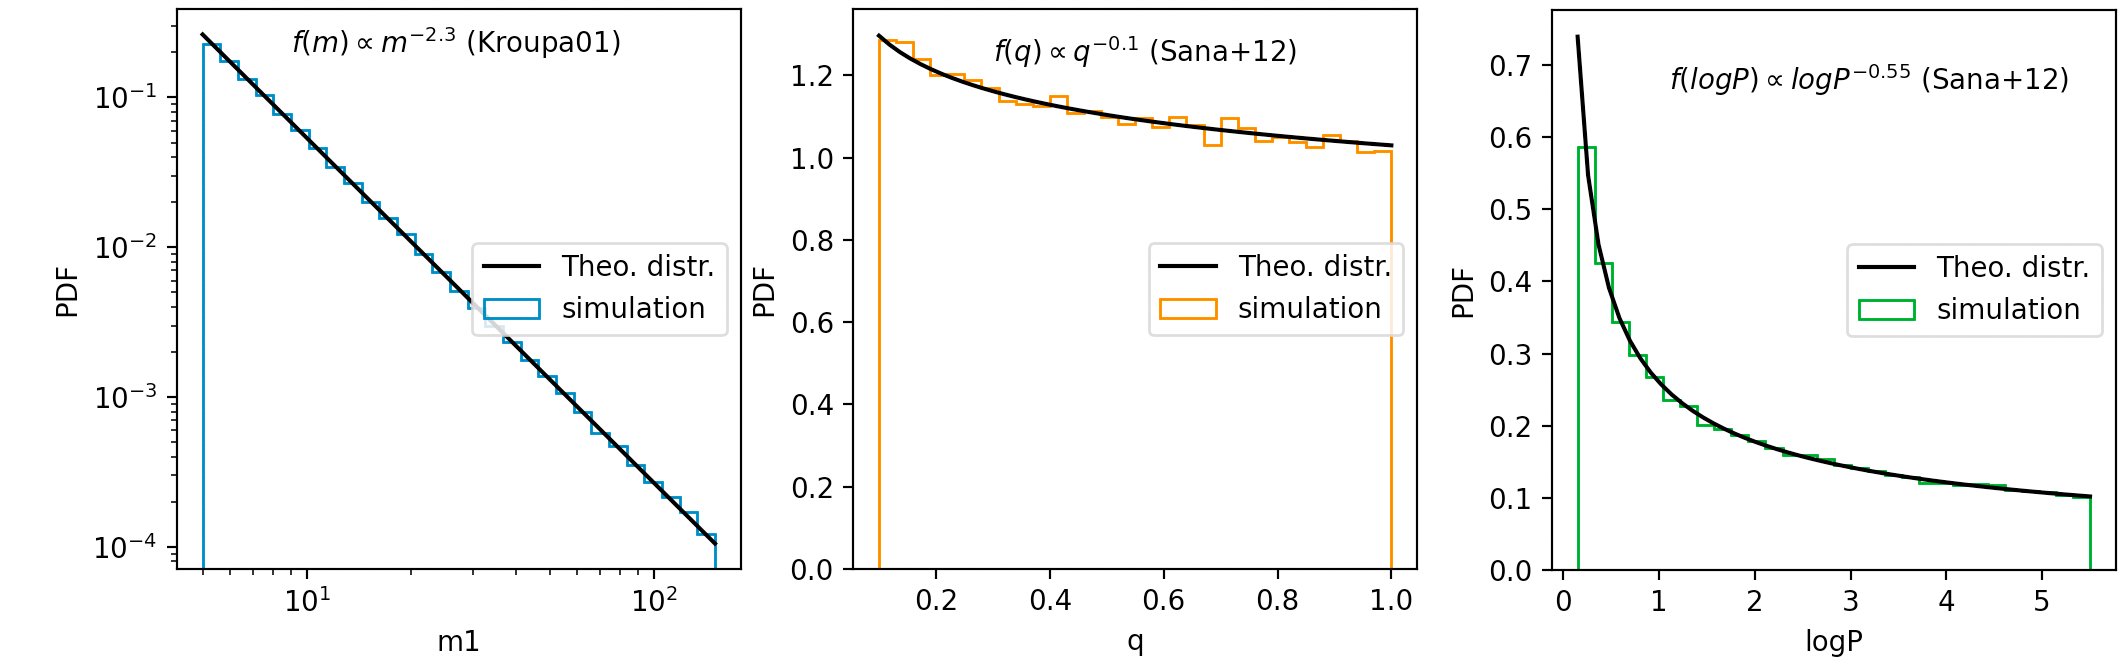
\includegraphics[width=\textwidth]{./images/initialconditions.png}\\
				\bigskip
				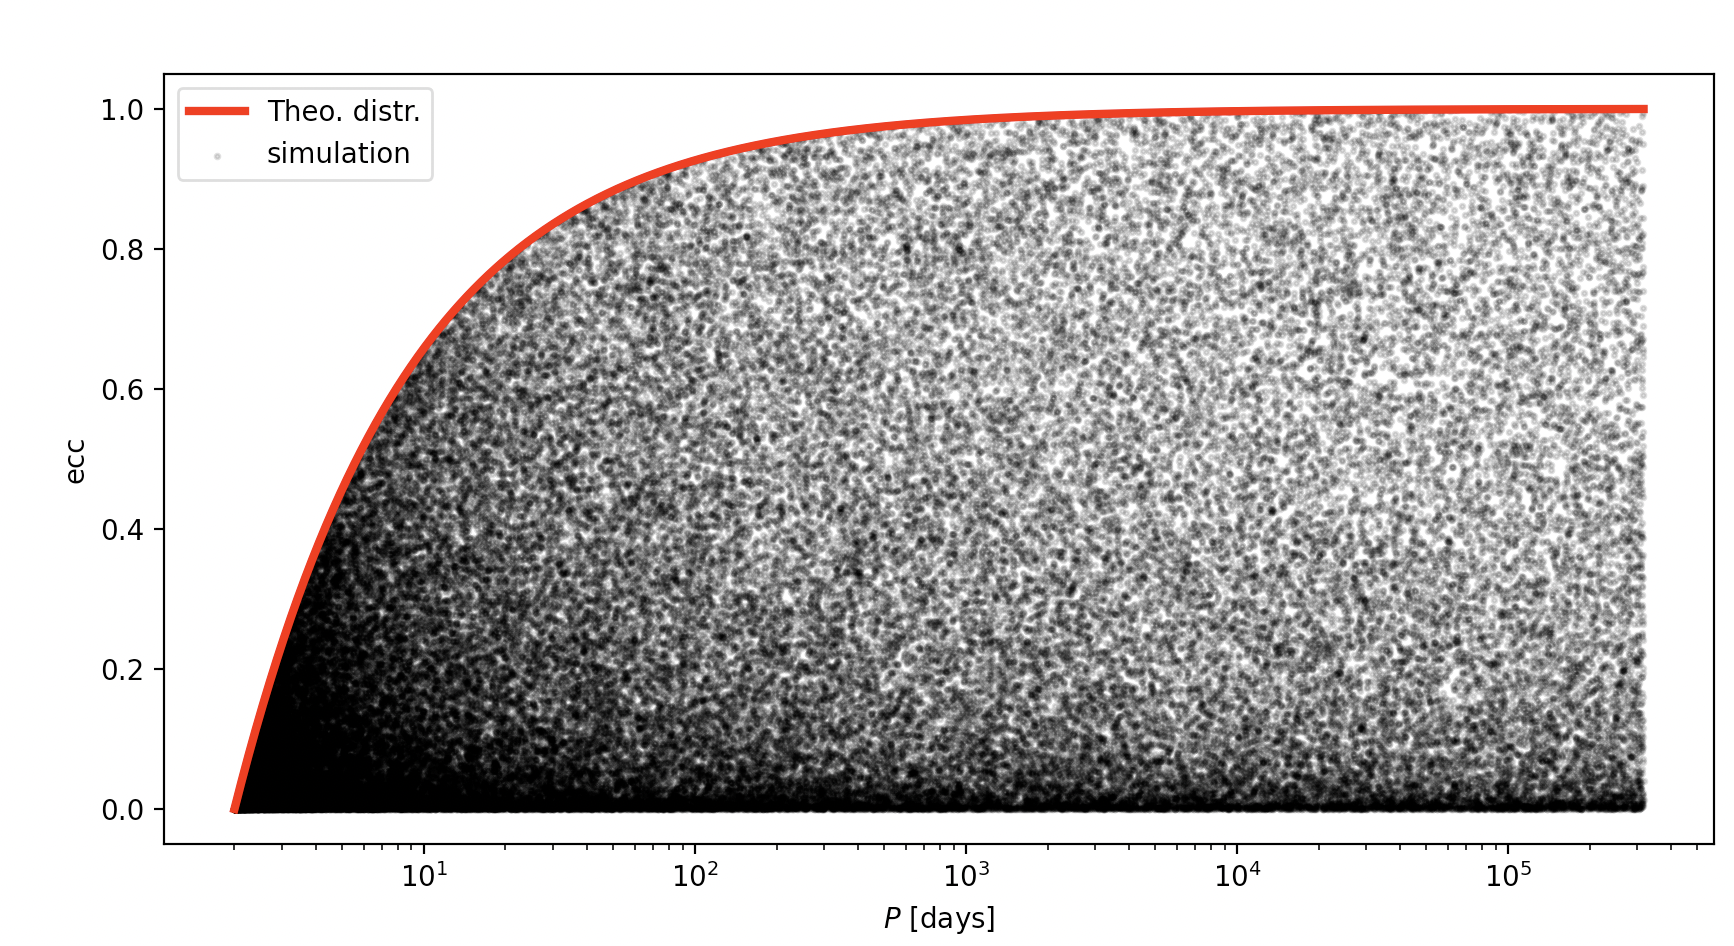
\includegraphics[width=\textwidth]{./images/initialperiods.png}
		\end{column}
	\end{columns}
\end{frame}




\begin{frame}[noframenumbering]{Results (1)}
	\scriptsize
	\begin{tabular}{l rrr>{\hspace{1.5pc}}rrr}
		\toprule
		Metallicity & \multicolumn{3}{c}{$Z=0.02$} & \multicolumn{3}{c}{$Z=0.015$}  \\
		%\midrule
		CCSN model & Rap & Del & Com &  Rap & Del & Com\\
		\toprule
		\toprule
		Natal kick model & \multicolumn{6}{c}{Maxwellian ($\sigma{}=70$ km/s)}
		\\
		\toprule
		BBHs  		                    & 5626 & 5248 & 18425 & 10350 & 7564 & 27740 \\
		after a WR--BH			& 100\% & 100\% & 100\% & 99\% & 99\%& 100\% \\
		\hline
		GW--BBHs  						& 207 & 171 & 949 & 418 & 282 & 1287 \\
		after a WR--BH				& 207 & 171 & 948 & 418 & 281 & 1285 \\
		\hline
		Cyg X-3 candidates 	 		& 14 & 8 & 76 & 16 & 10 & 18 \\
		becoming GW--BBHs   			& 14 & 6 & 76 & 16 & 9 & 18 \\
		\bottomrule 	
		\toprule
		Natal kick model & \multicolumn{6}{c}{Maxwellian ($\sigma{}=265$ km/s)}\\
		\toprule
		BBHs                        & 166 & 156 & 727  & 416 & 260 & 1420 \\
		after a WR--BH	  & 100\% & 100\% &  100\% & 99\% & 99\%&  100\% \\
		\hline
		GW--BBHs  		          & 34 & 21 & 221 & 101 & 67 &  392\\
		after a WR--BH	  & 34 & 21 &  221& 101 & 67 &  392\\
		\hline
		Cyg X-3 candidates  	  & 4 & 2 & 29 & 6 & 4 &  7\\
		becoming GW--BBHs   	  & 4 & 0 & 23 & 5 & 3 & 7 \\
		\bottomrule 	
	\end{tabular}%hobbspure265
\end{frame}

\begin{frame}[noframenumbering]{Results (2)}
	\scriptsize
		\begin{tabular}{l rrr>{\hspace{1.5pc}}rrr}
		\toprule
		Metallicity & \multicolumn{3}{c}{$Z=0.02$} & \multicolumn{3}{c}{$Z=0.015$}  \\
		%\midrule
		CCSN model & Rap & Del & Com &  Rap & Del & Com\\
		\toprule
		Natal kick model & \multicolumn{6}{c}{Maxwellian + fallback}\\
		\toprule
		BBHs                      		& 44307 & 35029 & 96557 & 55986 & 45701 & 109935 \\
		after a WR--BH			& 100\% & 100\% & 96\% & 92\% & 96\% & 94\% \\
		\hline
		GW--BBHs  						& 70 & 108 & 271 & 230 & 173 & 201 \\
		after a WR--BH			& 70 & 108 & 257 & 225 & 168 & 189 \\
		\hline
		Cyg X-3 candidates  	 		& 15 & 6 & 70 & 19 & 12 & 22 \\
		becoming GW--BBHs   		 	& 15 & 5 & 70 & 19 & 9 & 22 \\
		\bottomrule 	
		\toprule
		Natal kick model & \multicolumn{6}{c}{Unified}
		\\
		\toprule
		BBHs  		& 55655 & 46373 & 142613 & 71016 & 61257 & 157671 \\
		after a WR--BH	& 90\% & 95\% & 68\% & 87\% & 88\%& 69\% \\
		\hline
		GW--BBHs  		& 45 & 62 & 246 & 74 & 76 & 177 \\
		after a WR--BH	& 45 & 57 & 244 & 73 & 73 & 177 \\
		\hline
		Cyg X-3 candidates  	 & 16 & 7 & 70 & 19 & 9 & 22 \\
		becoming GW--BBHs   		 & 16 & 6 & 70 & 19 & 9 & 22 \\
		\bottomrule 	
	\end{tabular}%unified265
\end{frame}




\begin{frame}[noframenumbering]{Merger redshift and metallicity }
\centering
$\sim 10\%$ of today's BBH mergers have solar metallicity\\
\bigskip
\bigskip
	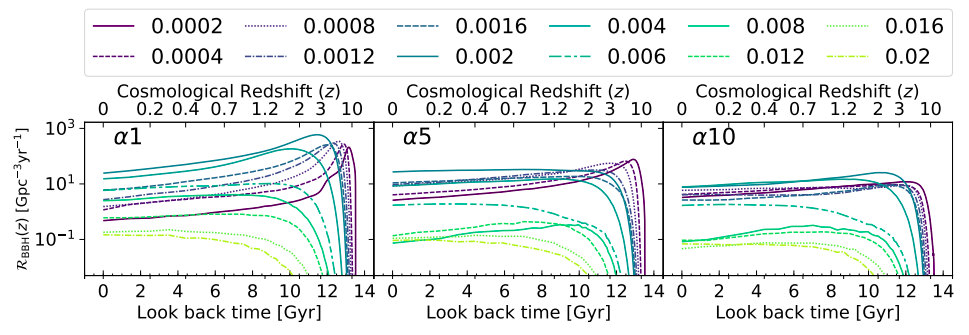
\includegraphics[width=\textwidth]{./images/redshift.png}\\
\smallskip
\referenza{Santoliquido et al. 2021}
\end{frame}

\begin{frame}[noframenumbering]{Fiducial evolution of Cyg X-3}
	\centering
	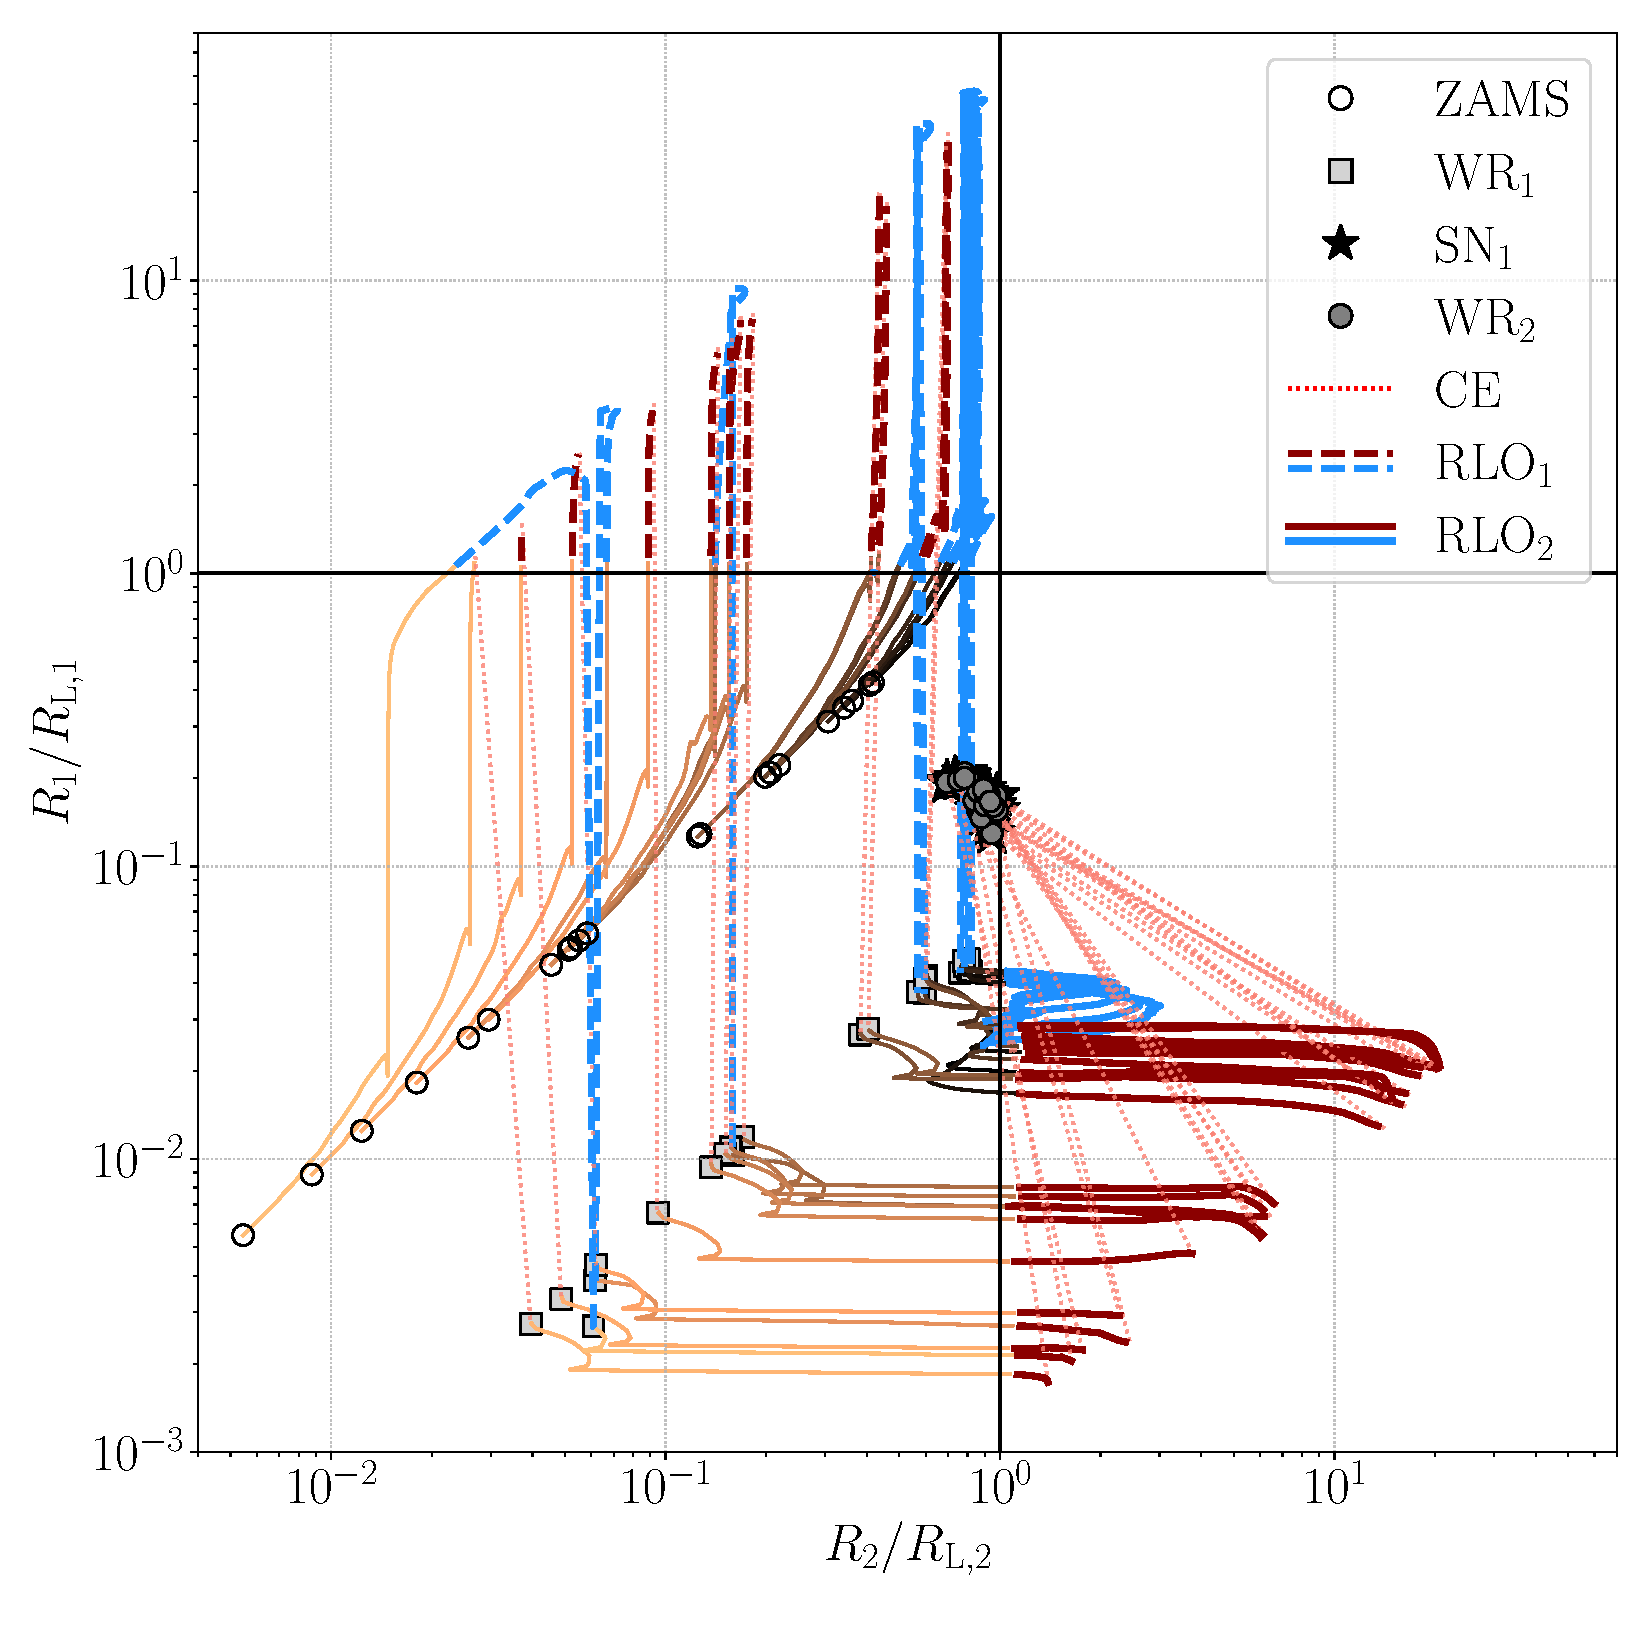
\includegraphics[width=.8\textwidth]{./images/RLfill1_RLfill0_BHBH_GW_WRBH_cyg_x-3--Ko17.pdf}
\end{frame}


\begin{frame}[noframenumbering]{Observability of Cyg X-3}
	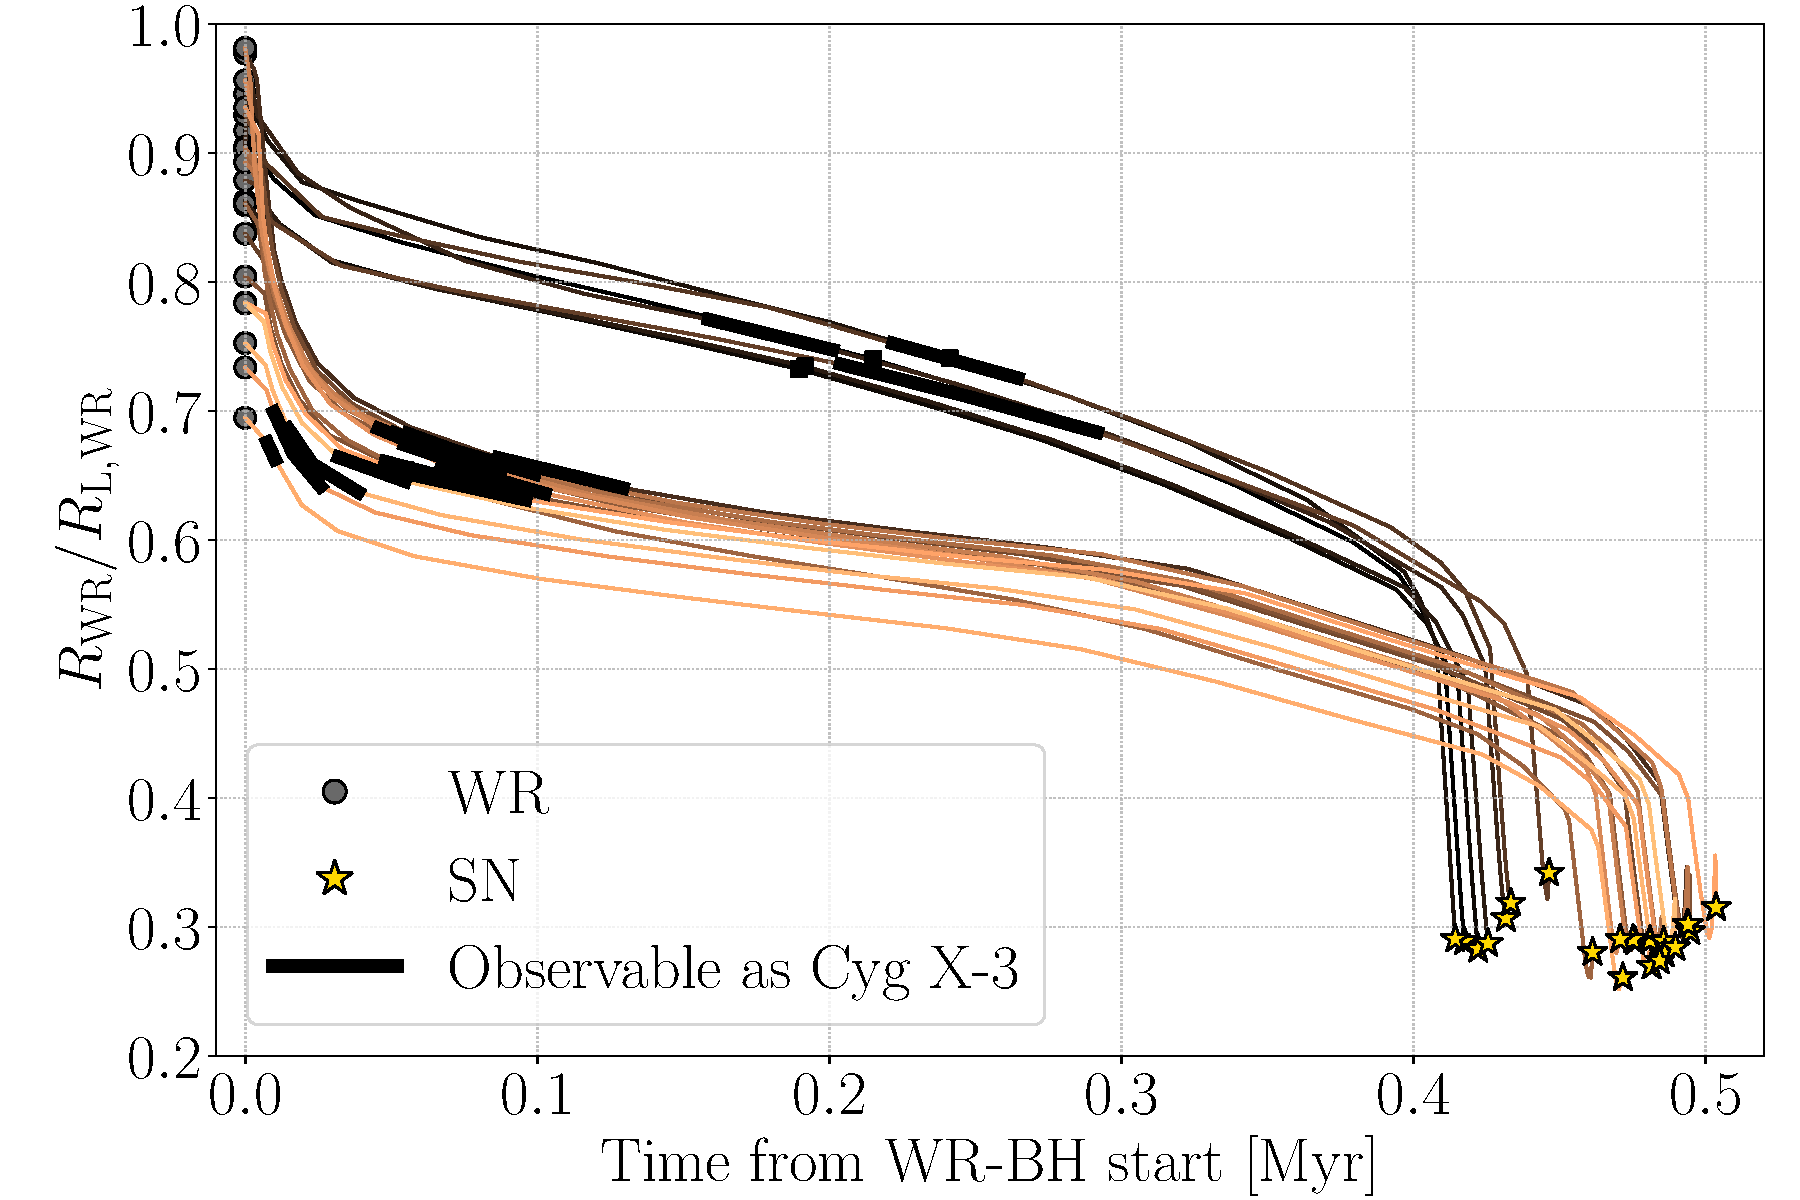
\includegraphics[width=\textwidth]{./images/BWorldtime_RLfill1_BHBH_GW_WRBH_cyg_x-3--Ko17.pdf}
\end{frame}



\begin{frame}[noframenumbering]{Influence of the parameter space}
	\small
	\begin{columns}
		\begin{column}{0.59\textwidth}
			\evidenzia{\textbf{Metallicity}:}
			\begin{itemize}
				\item \textbf{Negligible impact} \\ ($Z_\odot$=0.02 vs $Z_\odot$=0.015)
				\item $\neq$ number of systems, $\approx$ probability
			\end{itemize}
			\bigskip
			\evidenzia{\textbf{Kick}}
			\begin{itemize}
				\item \textbf{Strong kicks} $\rightarrow$ $\bm{e}_{\textbf{BBH}} \sim \textbf{1}$ \textbf{probable} \\
				$t_{\text{GW}} \propto (1-e^2)^{7/2}$ \referenza{Peters 1964}
				\item Merging BBHs for $a_{\text{BBH}} \lesssim 1000~R_\odot$
			\end{itemize}
			\bigskip
			\evidenzia{\textbf{Core-collapse supernova:}}
			\begin{itemize}
				\item \textbf{Compact object mass and nature}
				\item \textbf{Selects mass transfer evolution}
			\end{itemize}				
		\end{column}
		\begin{column}{0.5\textwidth}
			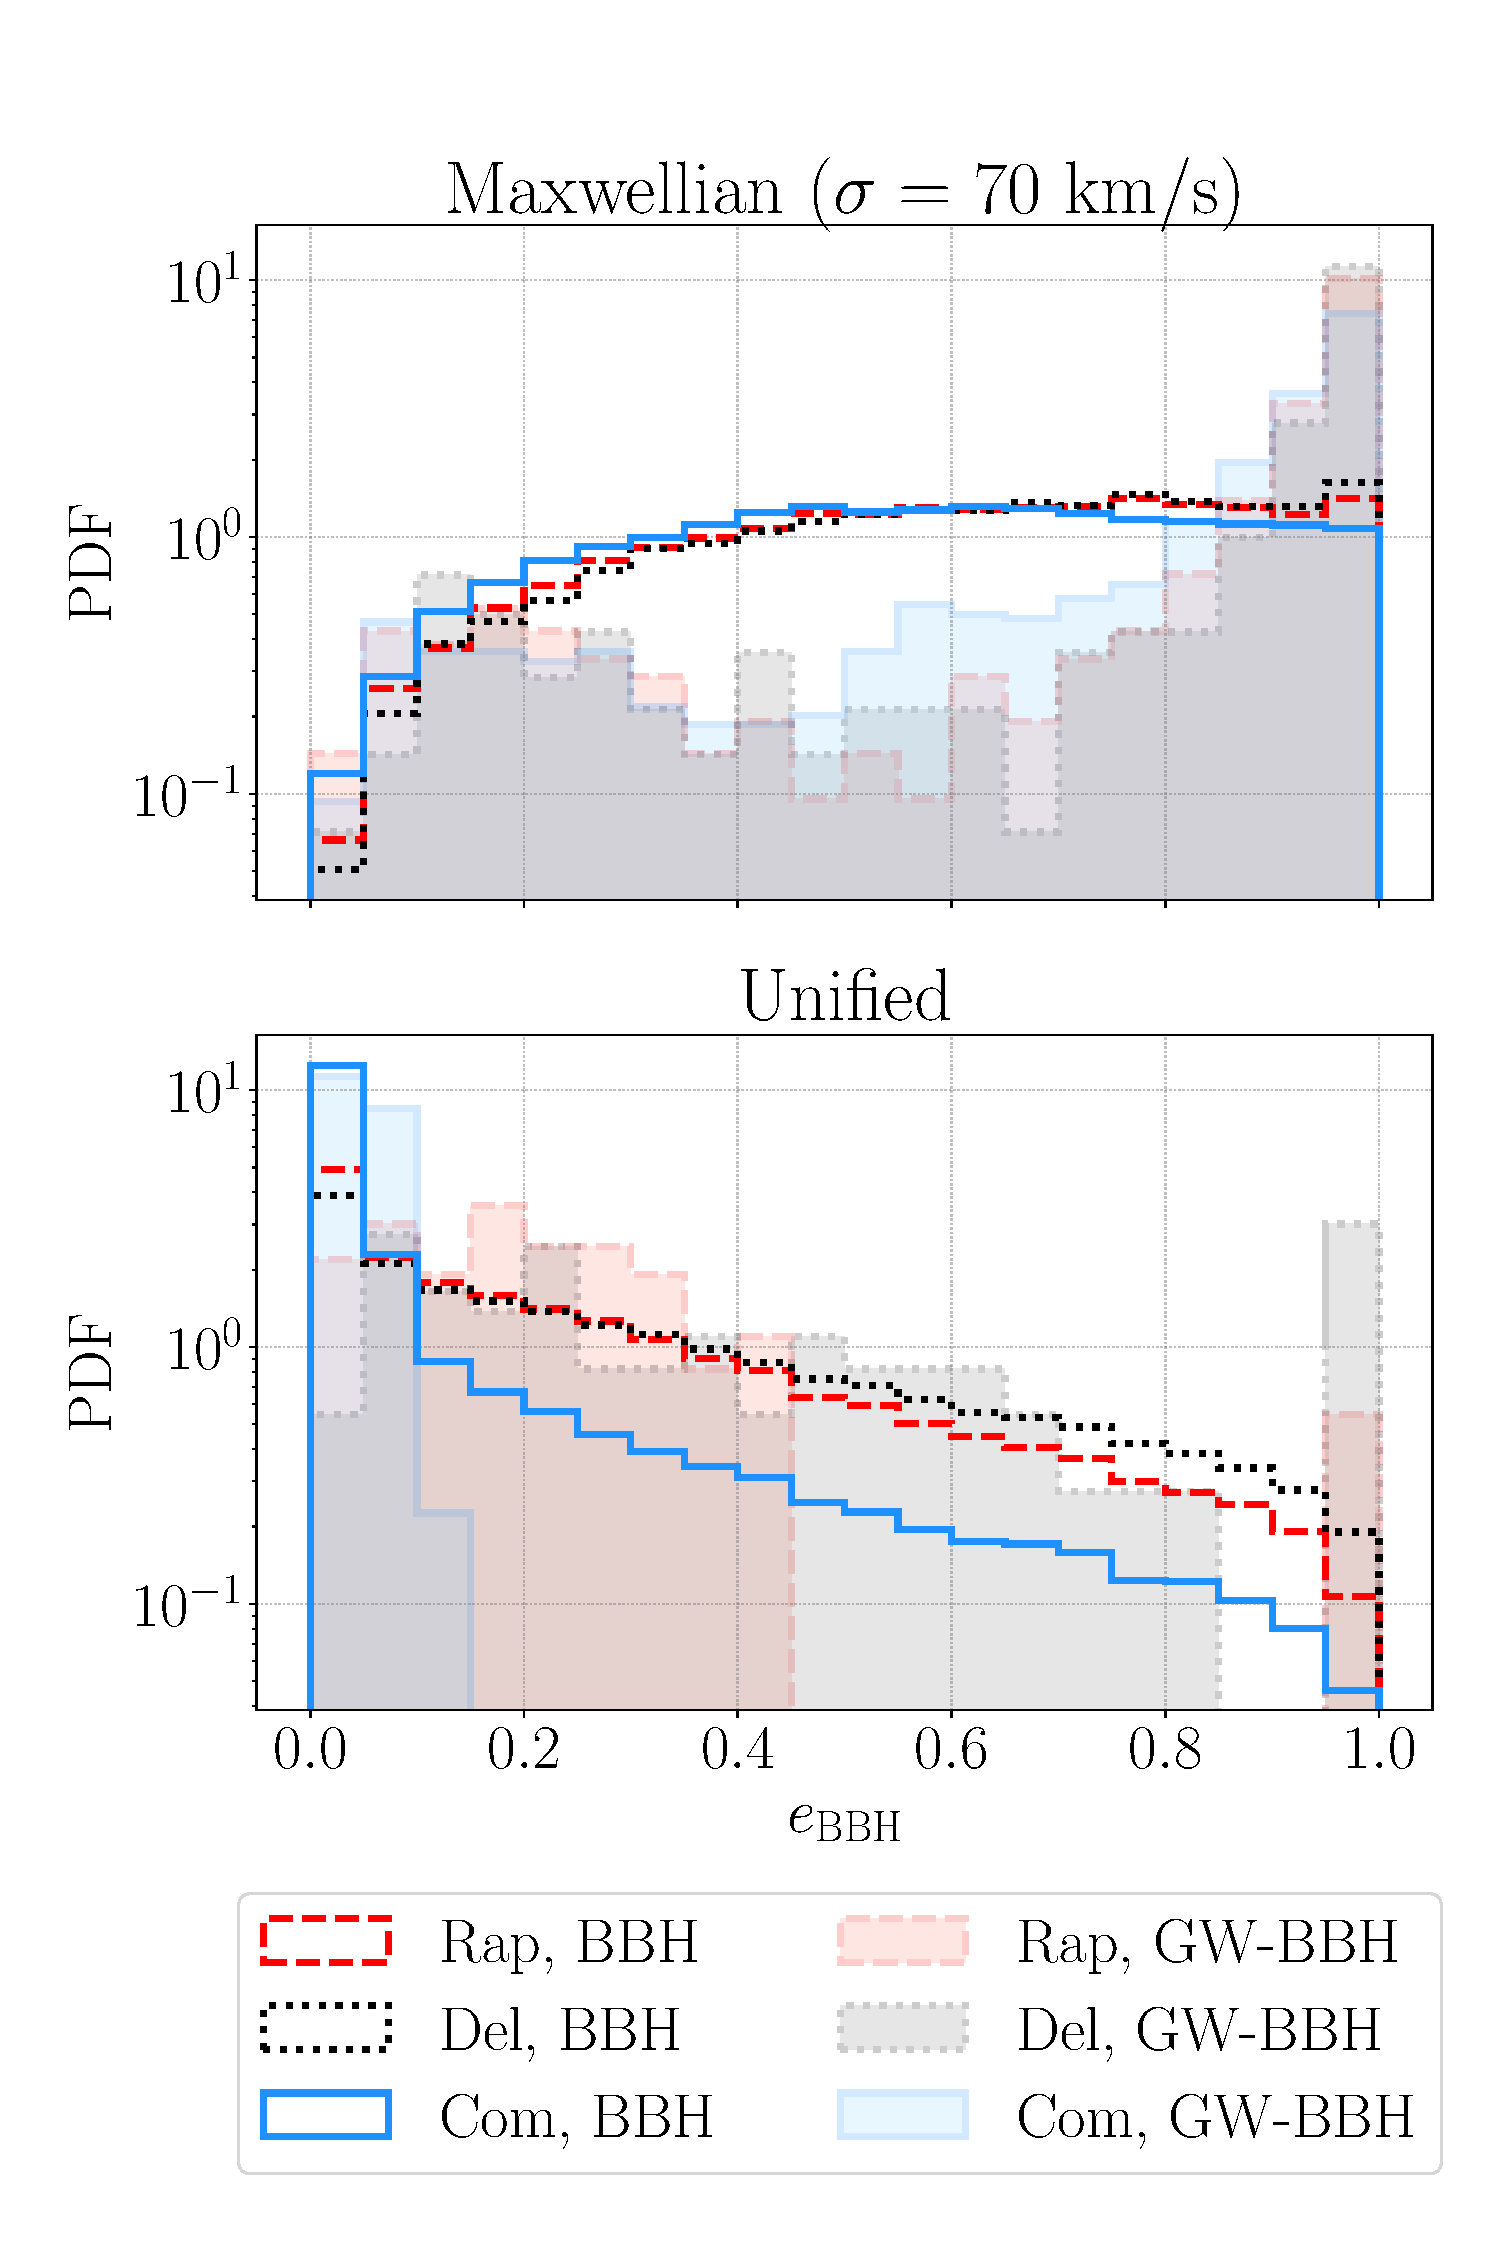
\includegraphics[width=\textwidth]{./images/remeccentricity_beamer.pdf}
		\end{column}	
	\end{columns}
\end{frame}


\begin{frame}[noframenumbering]{X-ray binaries and possible tensions}
	\begin{columns}
		\begin{column}{0.57\textwidth}
			\small
			\evidenzia{\textbf{High Mass X-ray binaries}}:
			\begin{itemize}
				\item accreting \textbf{black hole}
				\item \textbf{massive donor} ($\gtrsim 5~M_\odot$)
			\end{itemize}
			\bigskip
			\bigskip
			\smallskip
			
			\evidenzia{\textbf{Are progenitors of binary black holes?:}}\\
			\begin{itemize}
				\item Difficult to characterize (mass, spin)
				\item Compatible in the mass distribution
				\item \textbf{Tension in the spin distribution}
			\end{itemize}
			\bigskip
			\bigskip
			\centering
			\evidenzia{\textbf{The debate is still open!}}
		\end{column}
		\begin{column}{0.5\textwidth}
			\centering
			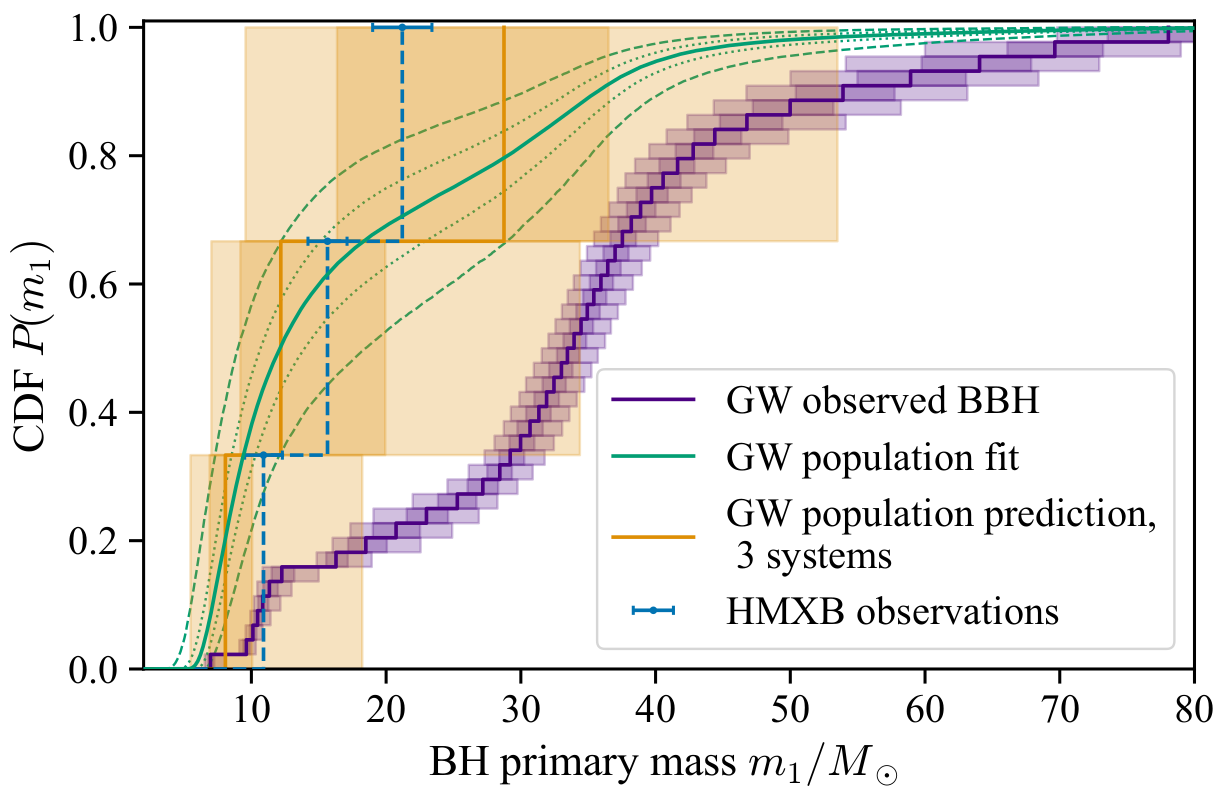
\includegraphics[width=.98\textwidth]{./images/tensionHMXBHmass.png}\acapo
			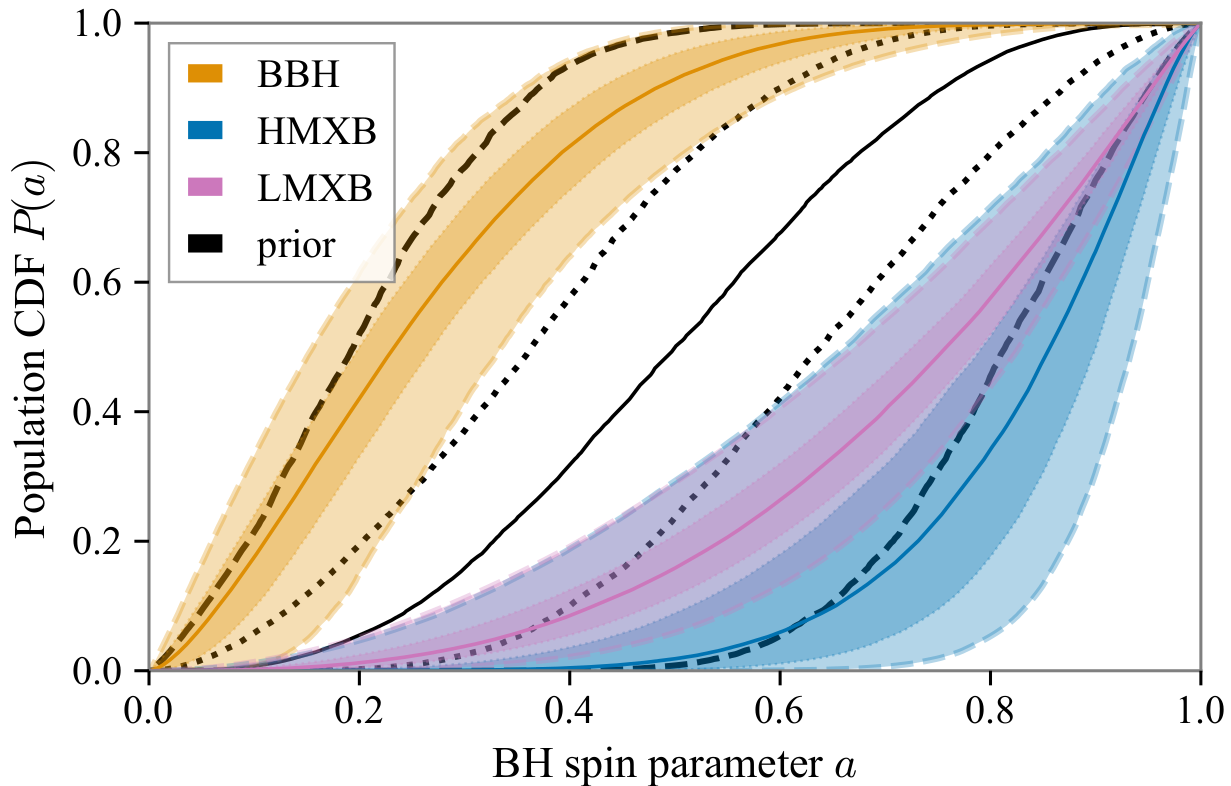
\includegraphics[width=.98\textwidth]{./images/tensionspin.png}
			\smallskip
			\referenza{Fishbach \& Kalogera 2022}
		\end{column}	
	\end{columns}
\end{frame}



\begin{frame}[noframenumbering]{\texttt{SEVN} speed}
	\centering
	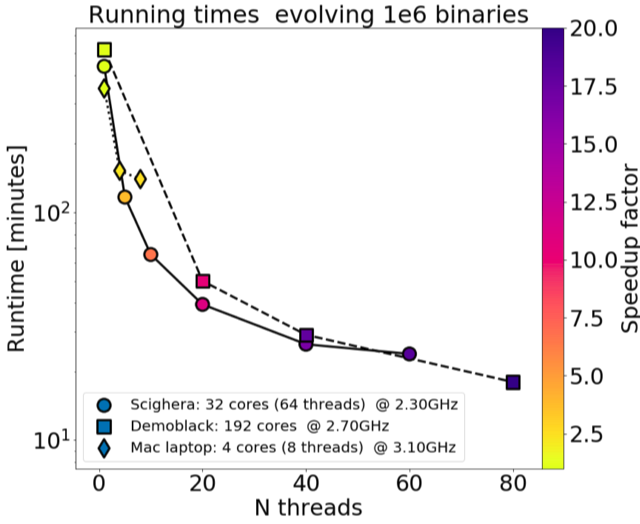
\includegraphics[width=.7\textwidth]{./images/SEVN.png}
\end{frame}


\end{document}
%%%%%%%%%%%%%%%%%%%%%%%%%%%%%%%%%%%%%%%%%%%%%%%%
%%%%%%%%%%%%%%%%%%%%%%%%%%%%%%%%%%%%%%%%%%%%%%%%
%%%%%%%%%%%%%%%%%%%%%%%%%%%%%%%%%%%%%%%%%%%%%%%%













\begin{frame}{Le binarie di oggetti compatti}
\framesubtitle{Introduzione ed evidenze osservative}

\evidenzia{Come si formano le binarie osservate tramite le onde gravitazionali?}

\bigskip

2 tipi di binarie di oggetti compatti: \referenza{Abbott et al., 2019} 
\begin{itemize}
	\item Binarie di buchi neri			\referenza{Abbott et al., 2016} 
	\item Binarie di stelle di neutroni \referenza{Abbott et al., 2017} 
\end{itemize}

\bigskip

Evoluzione difficile da prevedere e spiegare:
\begin{itemize}
	\item Sopravvivenza alle supernovae \\ $\rightarrow$ troppa massa espulsa slega il sistema \referenza{Pols, 2011}
	\item Coalescenza in $t < t_{\rm Hubble} \approx 13.6$ Gyr \\ $\rightarrow$ possibile solo per $a \lesssim 100 R_{\odot}$ \referenza{Peters, 1964}
\end{itemize}


\end{frame}



\begin{frame}{Scopo della tesi}\small
\framesubtitle{Simulazioni con SEVN}
%\vspace*{-8mm}
\evidenzia{Obiettivo:} Analizzare due processi critici per l'evoluzione delle binarie:
\begin{itemize}
	\item Il trasferimento di massa
	\item L'inviluppo comune
\end{itemize}

\medskip

	
\evidenzia{Metodo:} 
\begin{itemize}
\item Simulazione ed analisi di sistemi binari 
\item Codice di sintesi di popolazione: \referenza{Spera et al., 2015 }\\
SEVN  = ``\textit{Stellar EVolution for N-body simulations}''  \referenza{Spera et al., 2019}
\item Generazione di set con diversi parametri iniziali ($M$, $Z$, $a$):
	\begin{itemize}
		\item[$\bullet$] $M_1 = 26 M_\odot$, $30 M_\odot$, $35 M_\odot$
		\item[$\bullet$] $Z_{1,2} = 0.02$, $0.002$, $0.0002$
		\item[$\bullet$] $a = 100 R_\odot$, $500 R_\odot$, $1000 R_\odot$
	\end{itemize}
\end{itemize}

\end{frame}


\begin{frame}{Principi teorici}\normalsize
\framesubtitle{Trasferimento di massa}

\begin{columns}
\begin{column}{0.52\textwidth}
\begin{itemize}
	\item \textcolor{rossoPantano}{Vento stellare} \\ 
	Isotropo $\rightarrow$ inefficiente
	\vspace*{-2mm}
	{\footnotesize\[\langle\dot{M_2}\rangle \propto \! \left(\frac{v_\textup{orb}}{v_w}\right)^4 \!\dot{M_1} \qquad v_w \gg v_\textup{orb}\]}
	\item \textcolor{rossoPantano}{Roche lobe overflow (RLOF)}
	Flusso ordinato $\rightarrow$ efficiente
\begin{center}\vspace*{-3mm}
	\def\svgwidth{.8\textwidth}
	\import{./immagini/}{rlof_schema.pdf_tex}\hspace*{1cm}
\end{center}
	

\end{itemize}
\end{column}
\begin{column}{0.45\textwidth}
	\vspace*{-3mm}     %-8 se tolgo la cit
	\def\svgwidth{1.15\textwidth}
	\import{./immagini/}{rlof.pdf_tex} 
\end{column}	
\end{columns}

\flushleft
\tiny
\textit{Bondi \& Hoyle, 1944 - Hurley et al., 2002}
\end{frame}


\begin{frame}{Principi teorici}\large
\framesubtitle{Inviluppo comune}
\vspace*{-5mm}
\begin{columns}
\begin{column}{0.45\textwidth}
	\begin{itemize}
		\item \evidenzia{Inviluppo comune}
	\end{itemize}
\bigskip
\scriptsize
\centering
\def\svgwidth{\textwidth}
\import{./immagini/}{ce_schema_beamer.pdf_tex} 
\end{column}
\begin{column}{0.45\textwidth}
	\def\svgwidth{1.15\textwidth}
	\import{./immagini/}{ce_python.pdf_tex} 
\end{column}
\end{columns}
\tiny
\textit{Paczynski \& Ostriker, 1976 - Webbink, 1984} 	
\end{frame}



\begin{frame}{Risultati}
\framesubtitle{Influenza di trasferimento di massa e inviluppo comune}

\vspace*{-5mm}
\hspace*{18mm}\textcolor{rossoPantano}{2 inviluppi comuni \ \ \textit{vs} \ \ 2 Roche lobe overflow }

\medskip
\centering
\def\svgwidth{1.05\textwidth}
\import{./immagini/}{m_diverse4.pdf_tex} 
\end{frame}

\begin{frame}{Conclusioni}\scriptsize
\begin{columns}
	\begin{column}{0.49\textwidth}
		\textcolor{rossoPantano}{Scenario ideale}:
		\begin{enumerate}
			\item Orbita larga iniziale (100\,--1000 $R_{\odot}$)
			\item \evidenzia{RLOF}
			\item Primo oggetto compatto
			\item Binaria oggetto compatto + stella
			\item \evidenzia{Inviluppo comune}
			\item Secondo oggetto compatto
			\item \textbf{Binaria di oggetti compatti}
			\item \textbf{Coalescenza per emissione di GW}
		\end{enumerate}
	\end{column}
	\begin{column}{0.45\textwidth}
		\centering
		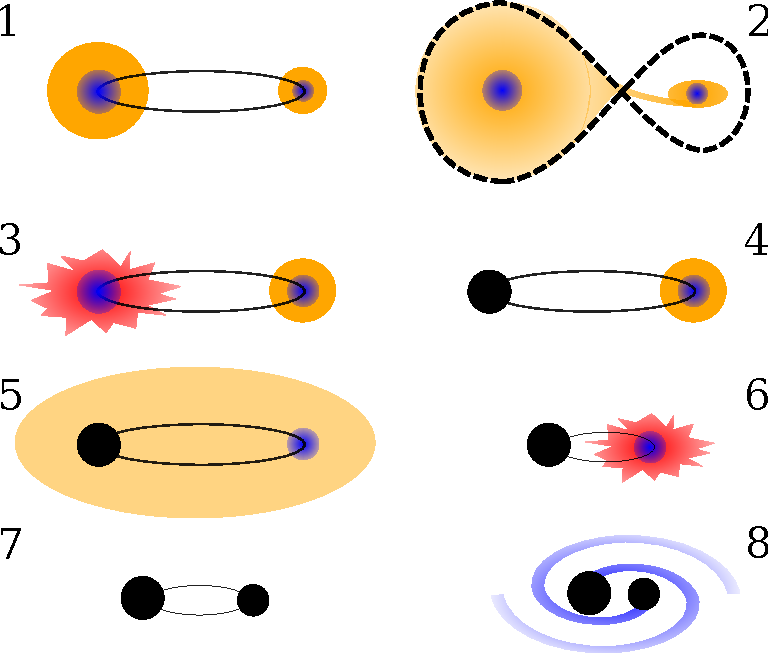
\includegraphics[width=0.87\textwidth]{./immagini/cartoon_finale.pdf}  %%%%%%%%% PIPPO troppo alta l-immagine rispetto alla linea di scenario ideale
	\end{column}
\end{columns}

\bigskip
\centering
\textcolor{rossoPantano}{Il trasferimento di massa e l'inviluppo comune possono spiegare gli eventi di coalescenza osservati a terra con le onde gravitazionali}\pause

\normalsize
\begin{center}
	\textbf{Grazie per l'attenzione}
\end{center}

\end{frame}


%%%%%%%%%%%%%%%%%%%%%%%%%%%%%%%%%%%%%%%%%%%%%%%%%%%%%%%%%%%%%
\begin{frame}[noframenumbering]{Set di simulazioni con SEVN}
\framesubtitle{Impatto della massa stellare}\footnotesize
\vspace*{-5mm}
\begin{figure}
	\centering
	\includegraphics[width=1.1\textwidth]{./immagini/sim_m.pdf}
\end{figure}
\end{frame}


\begin{frame}[noframenumbering]{Set di simulazioni con SEVN}
\framesubtitle{Impatto della metallicità stellare}\footnotesize
\vspace*{-5mm}
\begin{figure}
	\centering
	\includegraphics[width=1.1\textwidth]{./immagini/sim_z.pdf}
\end{figure}
\end{frame}

\begin{frame}[noframenumbering]{Set di simulazioni con SEVN}
\framesubtitle{Impatto del semiasse}\footnotesize
\vspace*{-5mm}
\begin{figure}
	\centering
	\includegraphics[width=1.1\textwidth]{./immagini/sim_a.pdf}
\end{figure}
\end{frame}

\begin{frame}[noframenumbering]{Tempo di coalescenza per emissione di GW}
\begin{equation*}
	t_{\rm GW} \sim \frac{5}{256} \frac{c^5}{G^3} \frac{a^4}{M_1 M_2 \left(M_1 + M_2\right)}
\end{equation*}\referenza{Peters, 1964}

\medskip

Per $M_1 = M_2 = 50 M_\odot$ e imponendo $t_{\rm GW} = t_{\rm Hubble} = 13.6$ Gyr \acapo
Si ottiene $a \sim 100 R_\odot$\acapo

Incompatibile con raggi stellari di 100\,-1000 $R_\odot$ (giganti)!

\bigskip

\centering
\begingroup
\renewcommand{\arraystretch}{1.4}
\begin{tabular}{ccc}
	\toprule
	Evento & $M_1$ ($M\sun$) & $M_2$ ($M\sun)$  \\
	\midrule
	GW170729 & $50.2^{+16.2}_{-10.2}$ & $34.0^{+9.1}_{-10.1}$ \\
	GW190521 & $85^{+21}_{-14}$ & $66^{+17}_{-18}$\\		
	\bottomrule
\end{tabular}
\endgroup


\end{frame}


\begin{frame}[noframenumbering]{Trasferimento conservativo}
\framesubtitle{Conseguenze orbitali}\footnotesize
\begin{columns}
	\begin{column}{0.52\textwidth}
			\evidenzia{Momento angolare orbitale}
		\begin{equation*}\footnotesize
		L = \mu\,v_\textup{orb}\,a = \frac{M_1 M_2}{M_1 + M_2} \sqrt{G \left(M_1 + M_2\right) a}
		\end{equation*}
		\evidenzia{Trasferimento conservativo se}
		\begin{equation*}\footnotesize
			\begin{cases}
			L=cost \\
			M_1 + M_2=cost
			\end{cases}
			\rightarrow
			\hspace{2mm}
			a \left(M_1M_2\right)^2 = cost
		\end{equation*}
		\evidenzia{Trasferimento non conservativo:}\\
		\[\text{se} \quad \left|\frac{dL}{L}\right| > \left|\frac{dM_1}{M_1}\right| \quad \rightarrow \quad \frac{da}{a} <0 \] \\
		\[\text{se} \quad \left|\frac{dL}{L}\right| < \left|\frac{dM_1}{M_1}\right| \quad \rightarrow \quad \frac{da}{a} >0 \]

	\end{column}
	\begin{column}{0.47\textwidth}
		\includegraphics[width=1.1\textwidth]{./immagini/a_mapelli.pdf}
		
		\bigskip
		\bigskip
		\bigskip
		\bigskip
		\tiny
		\textit{Hurley et al., 2002 - Immagine: Mapelli, 2020}
	\end{column}	
\end{columns}
\end{frame}


\begin{frame}[noframenumbering]{Massa trasferita}
\framesubtitle{Vento stellare e RLOF}\footnotesize
\vspace{-10mm}
\scriptsize	
\begin{columns}[t]
	\begin{column}{0.49\textwidth}
		\begin{center}
			\evidenzia{Vento stellare}
		\end{center}
		
		\textbf{Massa persa}
		\begin{equation*}
		\dot M \propto Z^{\alpha} \quad \alpha = 
		\begin{cases}
		0.85 & \Gamma_e < 2/3 \\
		2.45-2.4~\Gamma_e & 2/3 \leq \Gamma_e \leq 1
		\end{cases}
		\end{equation*}
		
		\begin{equation*}
		\begin{cases}
		\dot M \propto M^{0.68}\ \Gamma_e^{2.2} & 0.4 \lesssim \Gamma_e \lesssim 0.7 \\
		\dot M \propto M^{0.78}\ \Gamma_e^{4.77} & \Gamma_e \gtrsim 0.7
		\end{cases}
		\end{equation*}
		
		\textbf{Massa accresciuta mediamente}
		\begin{equation*}\footnotesize
		\langle \dot{M_2} \rangle \propto \left(\frac{v_\textup{orb}}{v_w}\right)^4 \dot{M_1} \quad v_w \gg v_\textup{orb}
		\end{equation*}
		
		\textbf{Tasso massimo accrezione} 
		\flushleft{$\dot{M}_\textup{Edd} = \frac{4 \pi c R}{k_\textup{es}}$}
		
		\smallskip
		\tiny
		\textit{Gr{\"a}fener \&  Hamann, 2008 - Vink et al., 2011 - Hurley et al., 2002}
	\end{column}
	\begin{column}{0.47\textwidth}
		\begin{center}
			\evidenzia{Roche lobe overflow}
		\end{center}
		
		\textbf{Raggio lobo di Roche}
		\begin{equation*}
		r_L = \frac{0.49~q^{2/3}}{0.6~q^{2/3} + \ln \left(1+q^{1/3}\right)}~a \quad q=\frac{M_1}{M_2}
		\end{equation*}
		
		\textbf{Massa persa}		
		\begin{equation*}
		\dot{M_1} = 3\cdot10^{-6} \left(\frac{M_1}{M\sun}\right)^2 \left[\ln\left(\frac{R_1}{r_{L,1}}\right)\right]^3
		\end{equation*}
		
		\textbf{Massa accresciuta}
		\begin{equation*}
		\dot{M}_2 = 
		\begin{cases}
		f_{\rm MT}\,{}|\dot{M}_1| & \text{altrimenti} \\
		\min{(f_{\rm MT}\,{}|\dot{M}_1|,\dot{M}_\textup{Edd})} & \text{$M_2$ degenere}
		\end{cases}
		\end{equation*}
		
		in SEVN $f_{\rm MT} = 0.5$
		
		\bigskip
		\medskip
		\tiny
		\textit{Eggleton, 1983 - Spera et al., 2019 - Mapelli et al., 2020}
	\end{column}	
\end{columns}

\end{frame}







\begin{frame}[noframenumbering]{Stabilità del RLOF}
\framesubtitle{Influenza di raggio e nucleo}\footnotesize
\vspace{-10mm}
\begin{columns}[t]
	\begin{column}{0.49\textwidth}
		\begin{center}
			\evidenzia{Variazione del raggio stellare}
		\end{center}
		
		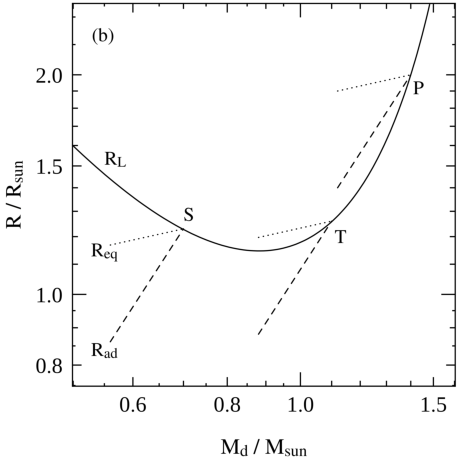
\includegraphics[width=0.9\textwidth]{./immagini/stp_roche.pdf}		
		\scriptsize
		\begin{equation*}
		\begin{cases}
			\text{stabile} &  \zeta_* \geq \zeta_L \\
			\text{instabile} &  \zeta_* \leq \zeta_L
		\end{cases}
		\quad \quad \zeta_{*,\evidenzia{L}} = \frac{d \ln R,\evidenzia{r_L}}{d \ln M}
		\end{equation*}
		\tiny
		\textit{Webbink, 1985 - Immagine: Pols, 2011}

		
	\end{column}
	\begin{column}{0.49\textwidth}
		\begin{center}
			\evidenzia{Frazione del nucleo di elio}
		\end{center}
		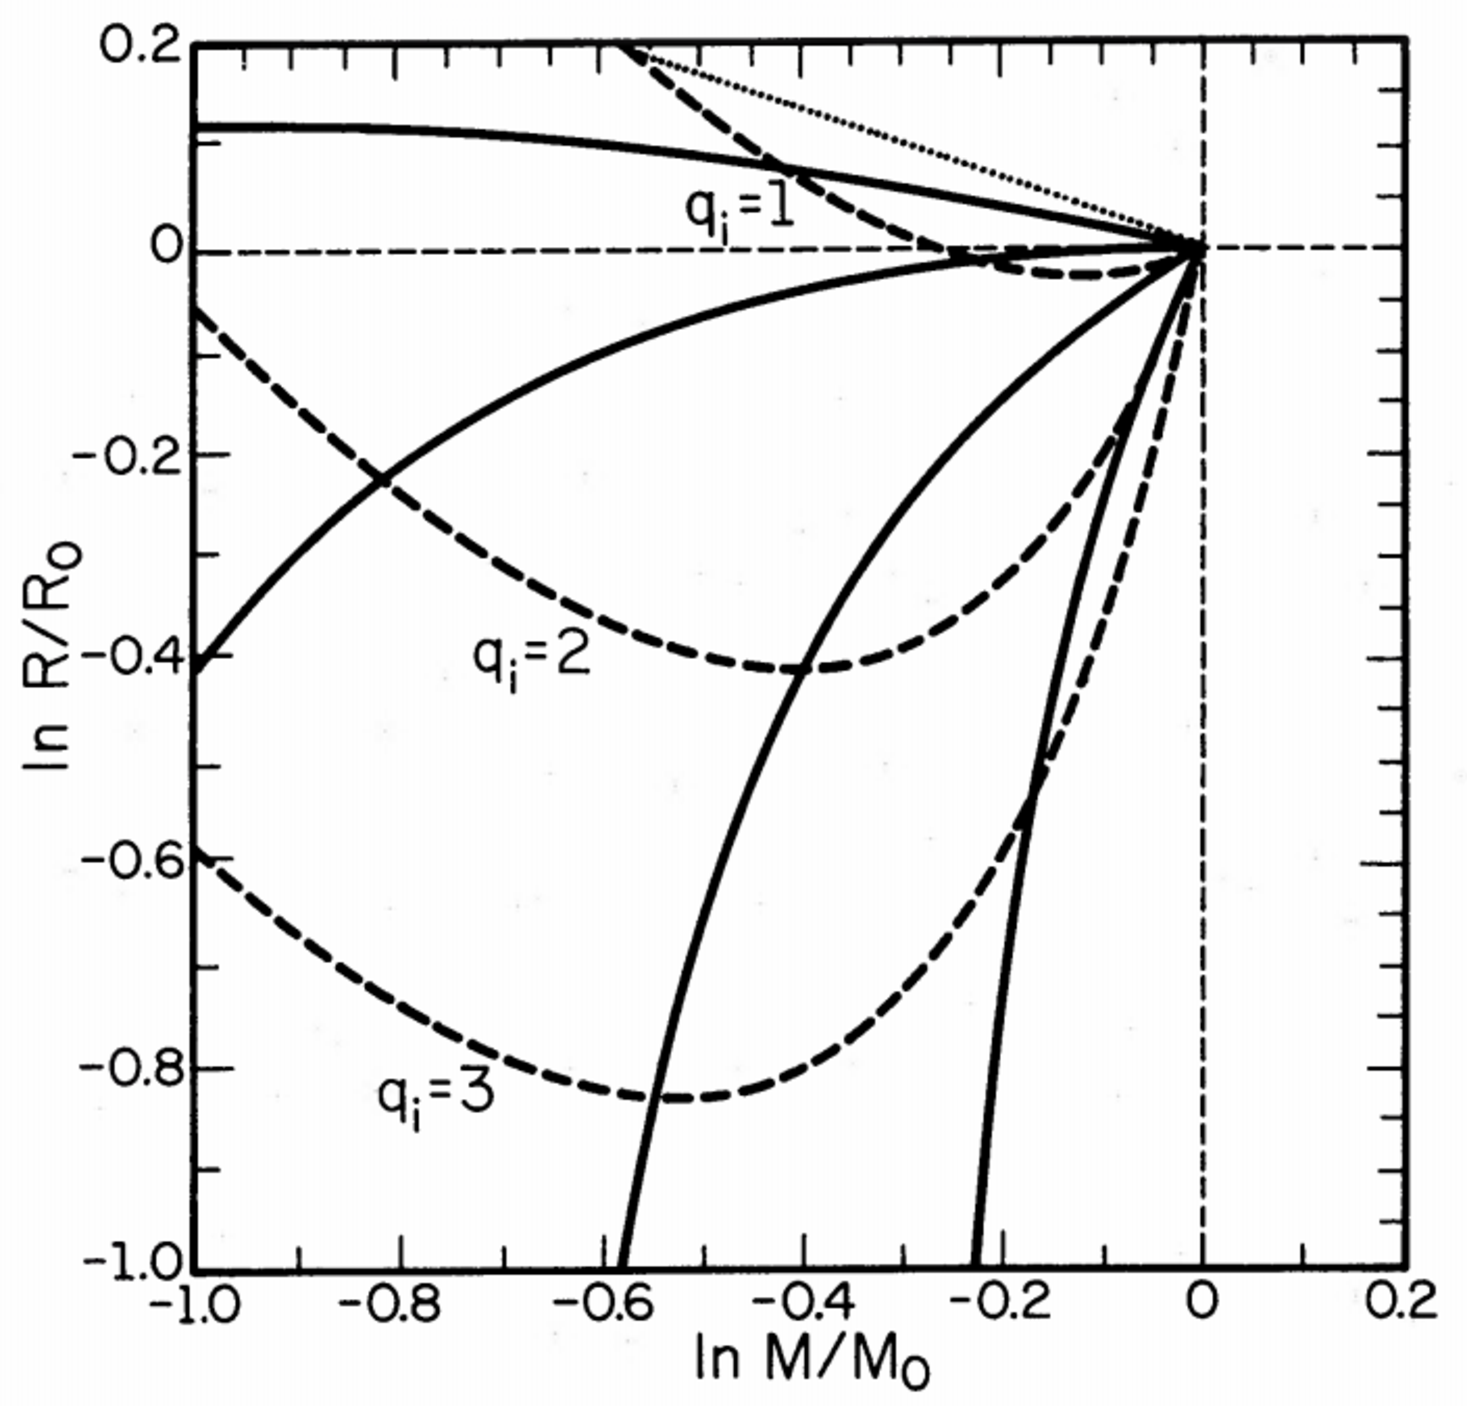
\includegraphics[width=0.9\textwidth]{./immagini/core_he_rlof.pdf}	
		
		\medskip
			
		\scriptsize
		\begin{equation*}
		q \geq q_\textup{crit} \left(q_\textup{core}\right) \quad \text{instabile}
		\end{equation*}
		
		\bigskip
		\tiny
		\textit{Immagine: Hjelliming \& Webbink, 1987}
	\end{column}	
\end{columns}
\end{frame}

\begin{frame}[noframenumbering]{Inviluppo comune}\scriptsize
\framesubtitle{Formalismo $\boldsymbol{\alpha \lambda}$}	
	\begin{columns}
		\begin{column}{0.6\textwidth}
			
			\textbf{Energia di legame dell'inviluppo comune}
			\begin{equation*}
			E_\textup{env} = - \frac{G}{\lambda} \left(\frac{m_\textup{env,1} M_1}{R_1}+ \frac{m_\textup{env,2} M_2}{R_2}\right)
			\end{equation*}
						
			\textbf{Variazione di energia orbitale}
			\begin{equation*}\scriptsize
			\Delta E_\textup{orb} = \alpha \left(E_\textup{orb, f} - E_\textup{orb, i}\right) = \alpha \frac{G M_\textup{c,1} M_\textup{c,2}}{2} \left(\frac{1}{a_\textup{i}} - \frac{1}{a_\textup{f}}\right)
			\end{equation*}
						
			\textbf{Semiasse finale imponendo $\Delta E_\textup{orb} = E_\textup{env}$}
			\begin{equation*}
			\frac{1}{a_\textup{f}} = \frac{1}{\alpha \lambda} \frac{2}{M_\textup{c,1} M_\textup{c,2}} \left(\frac{m_\textup{env,1} M_1}{R_1}+ \frac{m_\textup{env,2} M_2}{R_2}\right) + \frac{1}{a_\textup{i}}
			\end{equation*}
		\end{column}
		\begin{column}{0.45\textwidth}
			\includegraphics[width=1.05\textwidth]{./immagini/ce_appendice.pdf}
		\end{column}
	\end{columns}
\end{frame}



\end{document}